\documentclass[11pt]{article}
\usepackage[utf8]{inputenc}
\usepackage[T1]{fontenc}
\usepackage{textcomp}
\usepackage[a4paper,margin=2.1cm]{geometry}
\usepackage{amsmath,amssymb}
\usepackage{graphicx}
\usepackage{tikz}
\usetikzlibrary{arrows.meta}
\usepackage{xcolor}
\usepackage{mdframed}
\usepackage[colorlinks=true,linkcolor=blue!60!black]{hyperref}
\setlength{\parindent}{0pt}
\setlength{\parskip}{6pt}

\newcommand{\question}[1]{\par\medskip\noindent\textbf{#1}\par}
\newmdenv[linecolor=green!45!black,linewidth=0.8pt,backgroundcolor=green!4,
  innertopmargin=4pt,innerbottommargin=4pt,skipabove=6pt,skipbelow=6pt]{answerbox}

\title{\textbf{Equations of Straight Lines}\\[0.3em]\large Worked Solutions with TikZ Graphs}
\author{Wisest Maths --- Year 1 A-Level, Coordinate Geometry (ref \texttt{cg1})}
\date{}

\begin{document}
\maketitle
\noindent This document contains all 70 \emph{Equations of Straight Lines} questions, each with a
fully worked solution and a TikZ diagram drawn on the coordinate plane: the line(s) are plotted from their
equations, together with the given points, intercepts, midpoints, intersections, and (where relevant)
triangles, a circle, or a perpendicular foot.
\tableofcontents
\bigskip
\hrule

\section*{Equation of a Straight Line 01\quad\small\texttt{(cg1-001)}}
\addcontentsline{toc}{section}{Equation of a Straight Line 01 (cg1-001)}
\textit{Difficulty: Foundation \quad\textbar\quad Marks: 2}

\question{Write down the gradient and \( y \)-intercept of the line \( y = 3x - 7 \).}

\textbf{Worked solution.}

\textit{Compare with \( y = mx + c \).}
\[\begin{gathered}
y = 3x - 7 \implies m = 3,\ c = -7
\end{gathered}\]
The coefficient of \( x \) is the gradient; the constant is the \( y \)-intercept.

\begin{answerbox}
\textbf{Final answer:}\quad Gradient = \(\displaystyle 3\), y-intercept = \(\displaystyle (0, -7)\)
\end{answerbox}
\textbf{Diagram.}

\begin{center}
\resizebox{\ifdim\width>\linewidth \linewidth\else \width\fi}{!}{%
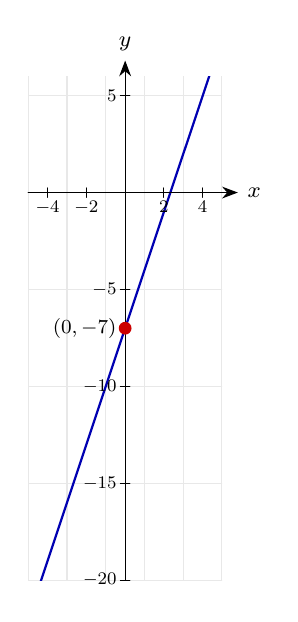
\begin{tikzpicture}[>={Stealth[length=2mm]},font=\footnotesize,line cap=round]
\begin{scope}
\clip (0,0) rectangle (2.462,6.4);
\draw[gray!18] (-0.246,0) grid[xstep=0.492,ystep=1.231] (2.462,6.4);
\draw[blue!70!black,thick] (0,-0.492) -- (2.462,6.892);
\end{scope}
\draw[->] (0,4.923) -- (2.662,4.923) node[right]{$x$};
\draw[->] (1.231,0) -- (1.231,6.6) node[above]{$y$};
\draw (0.246,4.863) -- (0.246,4.983) node[below=2pt,scale=0.8]{$-4$};
\draw (0.738,4.863) -- (0.738,4.983) node[below=2pt,scale=0.8]{$-2$};
\draw (1.723,4.863) -- (1.723,4.983) node[below=2pt,scale=0.8]{$2$};
\draw (2.215,4.863) -- (2.215,4.983) node[below=2pt,scale=0.8]{$4$};
\draw (1.171,0) -- (1.291,0) node[left=2pt,scale=0.8]{$-20$};
\draw (1.171,1.231) -- (1.291,1.231) node[left=2pt,scale=0.8]{$-15$};
\draw (1.171,2.462) -- (1.291,2.462) node[left=2pt,scale=0.8]{$-10$};
\draw (1.171,3.692) -- (1.291,3.692) node[left=2pt,scale=0.8]{$-5$};
\draw (1.171,6.154) -- (1.291,6.154) node[left=2pt,scale=0.8]{$5$};
\fill[red!80!black] (1.231,3.2) circle (2.3pt);
\node[left,scale=0.9] at (1.231,3.2) {$(0,-7)$};
\end{tikzpicture}
}
\end{center}
\small The line(s) and key points shown on the coordinate plane.\normalsize

\medskip\hrule

\section*{Equation of a Straight Line 02\quad\small\texttt{(cg1-002)}}
\addcontentsline{toc}{section}{Equation of a Straight Line 02 (cg1-002)}
\textit{Difficulty: Foundation \quad\textbar\quad Marks: 2}

\question{Write down the gradient and \( y \)-intercept of the line \( y = -2x + 5 \).}

\textbf{Worked solution.}

\textit{Compare with \( y = mx + c \).}
\[\begin{gathered}
y = -2x + 5 \implies m = -2,\ c = 5
\end{gathered}\]
The gradient is the coefficient of \( x \), which is negative here.

\begin{answerbox}
\textbf{Final answer:}\quad Gradient = \(\displaystyle -2\), y-intercept = \(\displaystyle (0, 5)\)
\end{answerbox}
\textbf{Diagram.}

\begin{center}
\resizebox{\ifdim\width>\linewidth \linewidth\else \width\fi}{!}{%
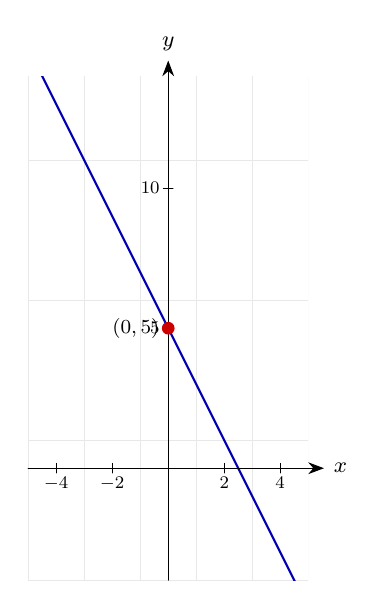
\begin{tikzpicture}[>={Stealth[length=2mm]},font=\footnotesize,line cap=round]
\begin{scope}
\clip (0,0) rectangle (3.556,6.4);
\draw[gray!18] (-0.356,-0.356) grid[xstep=0.711,ystep=1.778] (3.556,6.4);
\draw[blue!70!black,thick] (0,6.756) -- (3.556,-0.356);
\end{scope}
\draw[->] (0,1.422) -- (3.756,1.422) node[right]{$x$};
\draw[->] (1.778,0) -- (1.778,6.6) node[above]{$y$};
\draw (0.356,1.362) -- (0.356,1.482) node[below=2pt,scale=0.8]{$-4$};
\draw (1.067,1.362) -- (1.067,1.482) node[below=2pt,scale=0.8]{$-2$};
\draw (2.489,1.362) -- (2.489,1.482) node[below=2pt,scale=0.8]{$2$};
\draw (3.2,1.362) -- (3.2,1.482) node[below=2pt,scale=0.8]{$4$};
\draw (1.718,3.2) -- (1.838,3.2) node[left=2pt,scale=0.8]{$5$};
\draw (1.718,4.978) -- (1.838,4.978) node[left=2pt,scale=0.8]{$10$};
\fill[red!80!black] (1.778,3.2) circle (2.3pt);
\node[left,scale=0.9] at (1.778,3.2) {$(0,5)$};
\end{tikzpicture}
}
\end{center}
\small The line(s) and key points shown on the coordinate plane.\normalsize

\medskip\hrule

\section*{Equation of a Straight Line 03\quad\small\texttt{(cg1-003)}}
\addcontentsline{toc}{section}{Equation of a Straight Line 03 (cg1-003)}
\textit{Difficulty: Foundation \quad\textbar\quad Marks: 2}

\question{Write down the gradient and \( y \)-intercept of the line \( y = \dfrac{1}{3}x + 4 \).}

\textbf{Worked solution.}

\textit{Compare with \( y = mx + c \).}
\[\begin{gathered}
m = \tfrac{1}{3},\quad c = 4
\end{gathered}\]
The gradient is the fraction \( \frac{1}{3} \) and the \( y \)-intercept is 4.

\begin{answerbox}
\textbf{Final answer:}\quad Gradient = \(\displaystyle \dfrac{1}{3}\), y-intercept = \(\displaystyle (0, 4)\)
\end{answerbox}
\textbf{Diagram.}

\begin{center}
\resizebox{\ifdim\width>\linewidth \linewidth\else \width\fi}{!}{%
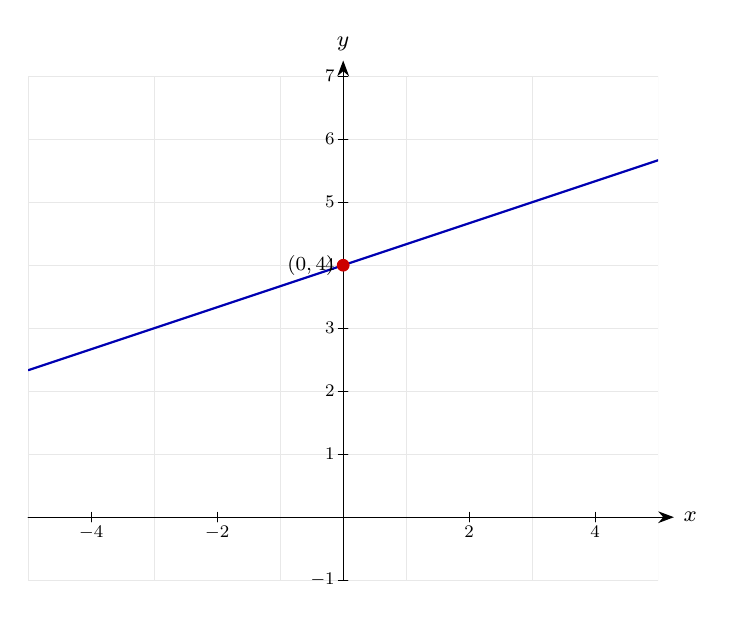
\begin{tikzpicture}[>={Stealth[length=2mm]},font=\footnotesize,line cap=round]
\begin{scope}
\clip (0,0) rectangle (8,6.4);
\draw[gray!18] (-0.8,0) grid[xstep=1.6,ystep=0.8] (8,6.4);
\draw[blue!70!black,thick] (0,2.667) -- (8,5.333);
\end{scope}
\draw[->] (0,0.8) -- (8.2,0.8) node[right]{$x$};
\draw[->] (4,0) -- (4,6.6) node[above]{$y$};
\draw (0.8,0.74) -- (0.8,0.86) node[below=2pt,scale=0.8]{$-4$};
\draw (2.4,0.74) -- (2.4,0.86) node[below=2pt,scale=0.8]{$-2$};
\draw (5.6,0.74) -- (5.6,0.86) node[below=2pt,scale=0.8]{$2$};
\draw (7.2,0.74) -- (7.2,0.86) node[below=2pt,scale=0.8]{$4$};
\draw (3.94,0) -- (4.06,0) node[left=2pt,scale=0.8]{$-1$};
\draw (3.94,1.6) -- (4.06,1.6) node[left=2pt,scale=0.8]{$1$};
\draw (3.94,2.4) -- (4.06,2.4) node[left=2pt,scale=0.8]{$2$};
\draw (3.94,3.2) -- (4.06,3.2) node[left=2pt,scale=0.8]{$3$};
\draw (3.94,4) -- (4.06,4) node[left=2pt,scale=0.8]{$4$};
\draw (3.94,4.8) -- (4.06,4.8) node[left=2pt,scale=0.8]{$5$};
\draw (3.94,5.6) -- (4.06,5.6) node[left=2pt,scale=0.8]{$6$};
\draw (3.94,6.4) -- (4.06,6.4) node[left=2pt,scale=0.8]{$7$};
\fill[red!80!black] (4,4) circle (2.3pt);
\node[left,scale=0.9] at (4,4) {$(0,4)$};
\end{tikzpicture}
}
\end{center}
\small The line(s) and key points shown on the coordinate plane.\normalsize

\medskip\hrule

\section*{Equation of a Straight Line 04\quad\small\texttt{(cg1-004)}}
\addcontentsline{toc}{section}{Equation of a Straight Line 04 (cg1-004)}
\textit{Difficulty: Foundation \quad\textbar\quad Marks: 2}

\question{Write down the equation of the straight line with gradient \( 4 \) and \( y \)-intercept \( (0, -1) \). Give your answer in the form \( y = mx + c \).}

\textbf{Worked solution.}

\textit{Substitute \( m = 4 \) and \( c = -1 \) into \( y = mx + c \).}
\[\begin{gathered}
y = 4x - 1
\end{gathered}\]
Direct substitution gives the equation.

\begin{answerbox}
\textbf{Final answer:}\quad \(\displaystyle y = 4x - 1\)
\end{answerbox}
\textbf{Diagram.}

\begin{center}
\resizebox{\ifdim\width>\linewidth \linewidth\else \width\fi}{!}{%
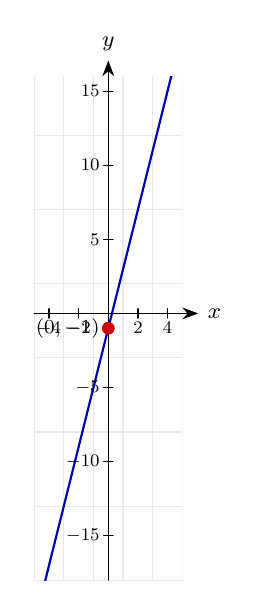
\begin{tikzpicture}[>={Stealth[length=2mm]},font=\footnotesize,line cap=round]
\begin{scope}
\clip (0,0) rectangle (1.882,6.4);
\draw[gray!18] (-0.188,-0.376) grid[xstep=0.376,ystep=0.941] (1.882,6.4);
\draw[blue!70!black,thick] (0,-0.565) -- (1.882,6.965);
\end{scope}
\draw[->] (0,3.388) -- (2.082,3.388) node[right]{$x$};
\draw[->] (0.941,0) -- (0.941,6.6) node[above]{$y$};
\draw (0.188,3.328) -- (0.188,3.448) node[below=2pt,scale=0.8]{$-4$};
\draw (0.565,3.328) -- (0.565,3.448) node[below=2pt,scale=0.8]{$-2$};
\draw (1.318,3.328) -- (1.318,3.448) node[below=2pt,scale=0.8]{$2$};
\draw (1.694,3.328) -- (1.694,3.448) node[below=2pt,scale=0.8]{$4$};
\draw (0.881,0.565) -- (1.001,0.565) node[left=2pt,scale=0.8]{$-15$};
\draw (0.881,1.506) -- (1.001,1.506) node[left=2pt,scale=0.8]{$-10$};
\draw (0.881,2.447) -- (1.001,2.447) node[left=2pt,scale=0.8]{$-5$};
\draw (0.881,4.329) -- (1.001,4.329) node[left=2pt,scale=0.8]{$5$};
\draw (0.881,5.271) -- (1.001,5.271) node[left=2pt,scale=0.8]{$10$};
\draw (0.881,6.212) -- (1.001,6.212) node[left=2pt,scale=0.8]{$15$};
\fill[red!80!black] (0.941,3.2) circle (2.3pt);
\node[left,scale=0.9] at (0.941,3.2) {$(0,-1)$};
\end{tikzpicture}
}
\end{center}
\small The line(s) and key points shown on the coordinate plane.\normalsize

\medskip\hrule

\section*{Equation of a Straight Line 05\quad\small\texttt{(cg1-005)}}
\addcontentsline{toc}{section}{Equation of a Straight Line 05 (cg1-005)}
\textit{Difficulty: Foundation \quad\textbar\quad Marks: 2}

\question{Write down the equation of the straight line with gradient \( -\dfrac{2}{3} \) and \( y \)-intercept \( (0, 6) \). Give your answer in the form \( y = mx + c \).}

\textbf{Worked solution.}

\textit{Substitute \( m = -\frac{2}{3} \) and \( c = 6 \).}
\[\begin{gathered}
y = -\dfrac{2}{3}x + 6
\end{gathered}\]
Direct substitution.

\begin{answerbox}
\textbf{Final answer:}\quad \(\displaystyle y = -\dfrac{2}{3}x + 6\)
\end{answerbox}
\textbf{Diagram.}

\begin{center}
\resizebox{\ifdim\width>\linewidth \linewidth\else \width\fi}{!}{%
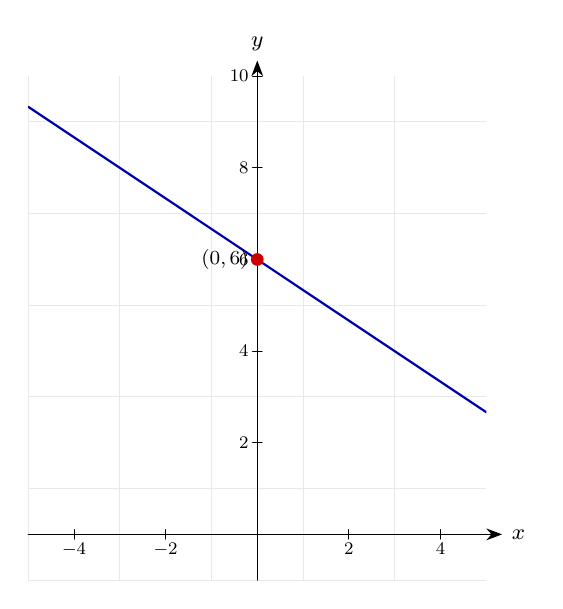
\begin{tikzpicture}[>={Stealth[length=2mm]},font=\footnotesize,line cap=round]
\begin{scope}
\clip (0,0) rectangle (5.818,6.4);
\draw[gray!18] (-0.582,-0.582) grid[xstep=1.164,ystep=1.164] (5.818,6.4);
\draw[blue!70!black,thick] (0,6.012) -- (5.818,2.133);
\end{scope}
\draw[->] (0,0.582) -- (6.018,0.582) node[right]{$x$};
\draw[->] (2.909,0) -- (2.909,6.6) node[above]{$y$};
\draw (0.582,0.522) -- (0.582,0.642) node[below=2pt,scale=0.8]{$-4$};
\draw (1.745,0.522) -- (1.745,0.642) node[below=2pt,scale=0.8]{$-2$};
\draw (4.073,0.522) -- (4.073,0.642) node[below=2pt,scale=0.8]{$2$};
\draw (5.236,0.522) -- (5.236,0.642) node[below=2pt,scale=0.8]{$4$};
\draw (2.849,1.745) -- (2.969,1.745) node[left=2pt,scale=0.8]{$2$};
\draw (2.849,2.909) -- (2.969,2.909) node[left=2pt,scale=0.8]{$4$};
\draw (2.849,4.073) -- (2.969,4.073) node[left=2pt,scale=0.8]{$6$};
\draw (2.849,5.236) -- (2.969,5.236) node[left=2pt,scale=0.8]{$8$};
\draw (2.849,6.4) -- (2.969,6.4) node[left=2pt,scale=0.8]{$10$};
\fill[red!80!black] (2.909,4.073) circle (2.3pt);
\node[left,scale=0.9] at (2.909,4.073) {$(0,6)$};
\end{tikzpicture}
}
\end{center}
\small The line(s) and key points shown on the coordinate plane.\normalsize

\medskip\hrule

\section*{Equation of a Straight Line 06\quad\small\texttt{(cg1-006)}}
\addcontentsline{toc}{section}{Equation of a Straight Line 06 (cg1-006)}
\textit{Difficulty: Foundation \quad\textbar\quad Marks: 2}

\question{Write down the equation of the straight line with gradient \( 0.5 \) and \( y \)-intercept \( (0, -3) \). Give your answer in the form \( y = mx + c \).}

\textbf{Worked solution.}

\textit{Substitute \( m = 0.5 \) and \( c = -3 \).}
\[\begin{gathered}
y = 0.5x - 3
\end{gathered}\]
Direct substitution gives the equation.

\begin{answerbox}
\textbf{Final answer:}\quad \(\displaystyle y = 0.5x - 3\)
\end{answerbox}
\textbf{Diagram.}

\begin{center}
\resizebox{\ifdim\width>\linewidth \linewidth\else \width\fi}{!}{%
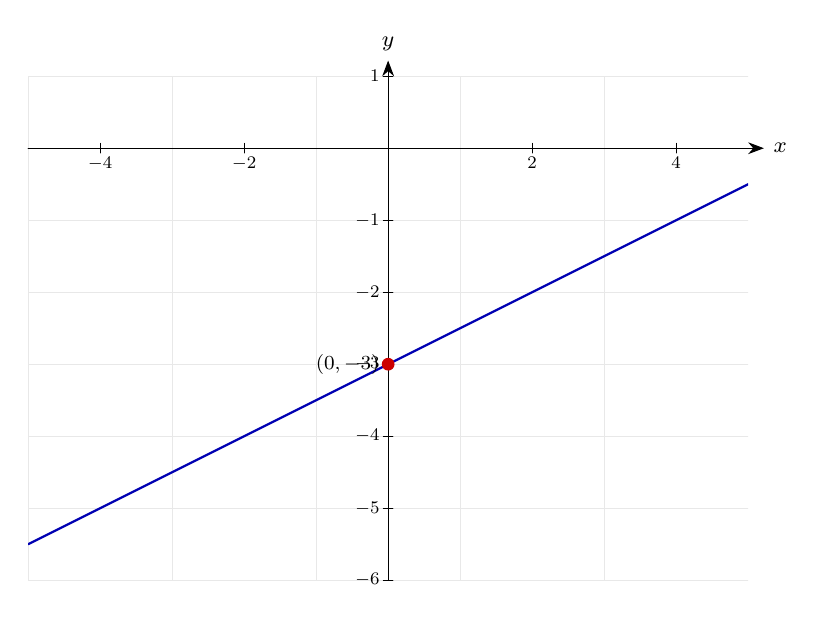
\begin{tikzpicture}[>={Stealth[length=2mm]},font=\footnotesize,line cap=round]
\begin{scope}
\clip (0,0) rectangle (9.143,6.4);
\draw[gray!18] (-0.914,0) grid[xstep=1.829,ystep=0.914] (9.143,6.4);
\draw[blue!70!black,thick] (0,0.457) -- (9.143,5.029);
\end{scope}
\draw[->] (0,5.486) -- (9.343,5.486) node[right]{$x$};
\draw[->] (4.571,0) -- (4.571,6.6) node[above]{$y$};
\draw (0.914,5.426) -- (0.914,5.546) node[below=2pt,scale=0.8]{$-4$};
\draw (2.743,5.426) -- (2.743,5.546) node[below=2pt,scale=0.8]{$-2$};
\draw (6.4,5.426) -- (6.4,5.546) node[below=2pt,scale=0.8]{$2$};
\draw (8.229,5.426) -- (8.229,5.546) node[below=2pt,scale=0.8]{$4$};
\draw (4.511,0) -- (4.631,0) node[left=2pt,scale=0.8]{$-6$};
\draw (4.511,0.914) -- (4.631,0.914) node[left=2pt,scale=0.8]{$-5$};
\draw (4.511,1.829) -- (4.631,1.829) node[left=2pt,scale=0.8]{$-4$};
\draw (4.511,2.743) -- (4.631,2.743) node[left=2pt,scale=0.8]{$-3$};
\draw (4.511,3.657) -- (4.631,3.657) node[left=2pt,scale=0.8]{$-2$};
\draw (4.511,4.571) -- (4.631,4.571) node[left=2pt,scale=0.8]{$-1$};
\draw (4.511,6.4) -- (4.631,6.4) node[left=2pt,scale=0.8]{$1$};
\fill[red!80!black] (4.571,2.743) circle (2.3pt);
\node[left,scale=0.9] at (4.571,2.743) {$(0,-3)$};
\end{tikzpicture}
}
\end{center}
\small The line(s) and key points shown on the coordinate plane.\normalsize

\medskip\hrule

\section*{Equation of a Straight Line 07\quad\small\texttt{(cg1-007)}}
\addcontentsline{toc}{section}{Equation of a Straight Line 07 (cg1-007)}
\textit{Difficulty: Foundation \quad\textbar\quad Marks: 3}

\question{Find the equation of the line that passes through the points \( (2, 5) \) and \( (6, 13) \). Write your answer in the form \( y - y_1 = m(x - x_1) \).}

\textbf{Worked solution.}

\textit{Find the gradient and write the equation.}
\[\begin{gathered}
\begin{aligned} m &= \dfrac{13 - 5}{6 - 2} = \dfrac{8}{4} = 2 \end{aligned}
\end{gathered}\]
Use \( m = \frac{y_2 - y_1}{x_2 - x_1} \). Then substitute into \( y - y_1 = m(x - x_1) \) using either point.

\begin{answerbox}
\textbf{Final answer:}\quad \(\displaystyle y - 5 = 2(x - 2)\) or equivalently \(\displaystyle y - 13 = 2(x - 6)\)
\end{answerbox}
\textbf{Common mistake.} Both answers are equally valid --- you can use either point in the formula.

\textbf{Diagram.}

\begin{center}
\resizebox{\ifdim\width>\linewidth \linewidth\else \width\fi}{!}{%
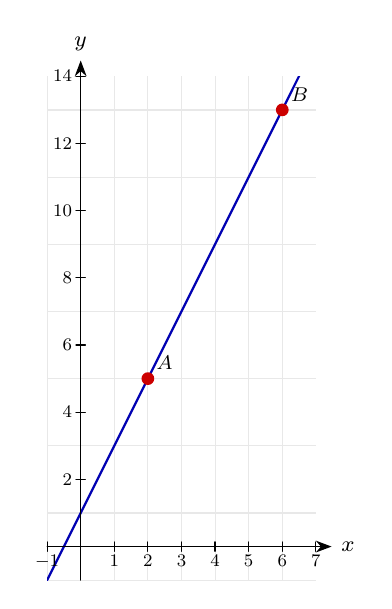
\begin{tikzpicture}[>={Stealth[length=2mm]},font=\footnotesize,line cap=round]
\begin{scope}
\clip (0,0) rectangle (3.413,6.4);
\draw[gray!18] (0,-0.427) grid[xstep=0.427,ystep=0.853] (3.413,6.4);
\draw[blue!70!black,thick] (0,0) -- (3.413,6.827);
\end{scope}
\draw[->] (0,0.427) -- (3.613,0.427) node[right]{$x$};
\draw[->] (0.427,0) -- (0.427,6.6) node[above]{$y$};
\draw (0,0.367) -- (0,0.487) node[below=2pt,scale=0.8]{$-1$};
\draw (0.853,0.367) -- (0.853,0.487) node[below=2pt,scale=0.8]{$1$};
\draw (1.28,0.367) -- (1.28,0.487) node[below=2pt,scale=0.8]{$2$};
\draw (1.707,0.367) -- (1.707,0.487) node[below=2pt,scale=0.8]{$3$};
\draw (2.133,0.367) -- (2.133,0.487) node[below=2pt,scale=0.8]{$4$};
\draw (2.56,0.367) -- (2.56,0.487) node[below=2pt,scale=0.8]{$5$};
\draw (2.987,0.367) -- (2.987,0.487) node[below=2pt,scale=0.8]{$6$};
\draw (3.413,0.367) -- (3.413,0.487) node[below=2pt,scale=0.8]{$7$};
\draw (0.367,1.28) -- (0.487,1.28) node[left=2pt,scale=0.8]{$2$};
\draw (0.367,2.133) -- (0.487,2.133) node[left=2pt,scale=0.8]{$4$};
\draw (0.367,2.987) -- (0.487,2.987) node[left=2pt,scale=0.8]{$6$};
\draw (0.367,3.84) -- (0.487,3.84) node[left=2pt,scale=0.8]{$8$};
\draw (0.367,4.693) -- (0.487,4.693) node[left=2pt,scale=0.8]{$10$};
\draw (0.367,5.547) -- (0.487,5.547) node[left=2pt,scale=0.8]{$12$};
\draw (0.367,6.4) -- (0.487,6.4) node[left=2pt,scale=0.8]{$14$};
\fill[red!80!black] (1.28,2.56) circle (2.3pt);
\node[above right,scale=0.9] at (1.28,2.56) {$A$};
\fill[red!80!black] (2.987,5.973) circle (2.3pt);
\node[above right,scale=0.9] at (2.987,5.973) {$B$};
\end{tikzpicture}
}
\end{center}
\small The line(s) and key points shown on the coordinate plane.\normalsize

\medskip\hrule

\section*{Equation of a Straight Line 08\quad\small\texttt{(cg1-008)}}
\addcontentsline{toc}{section}{Equation of a Straight Line 08 (cg1-008)}
\textit{Difficulty: Foundation \quad\textbar\quad Marks: 3}

\question{Find the equation of the line passing through \( (1, 7) \) and \( (4, 1) \). Write your answer in the form \( y - y_1 = m(x - x_1) \).}

\textbf{Worked solution.}

\textit{Find the gradient and write the equation.}
\[\begin{gathered}
\begin{aligned} m &= \dfrac{1 - 7}{4 - 1} = \dfrac{-6}{3} = -2 \end{aligned}
\end{gathered}\]
The gradient is negative, meaning the line slopes downward. Substitute into \( y - y_1 = m(x - x_1) \) using either point.

\begin{answerbox}
\textbf{Final answer:}\quad \(\displaystyle y - 7 = -2(x - 1)\) or equivalently \(\displaystyle y - 1 = -2(x - 4)\)
\end{answerbox}
\textbf{Common mistake.} Both answers are equally valid --- you can use either point in the formula.

\textbf{Diagram.}

\begin{center}
\resizebox{\ifdim\width>\linewidth \linewidth\else \width\fi}{!}{%
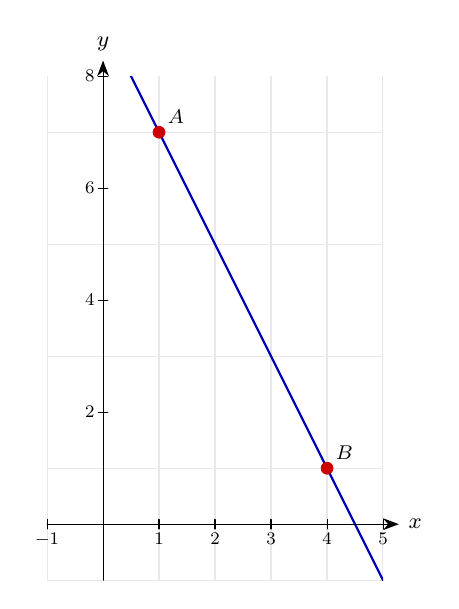
\begin{tikzpicture}[>={Stealth[length=2mm]},font=\footnotesize,line cap=round]
\begin{scope}
\clip (0,0) rectangle (4.267,6.4);
\draw[gray!18] (0,-0.711) grid[xstep=0.711,ystep=1.422] (4.267,6.4);
\draw[blue!70!black,thick] (0,8.533) -- (4.267,0);
\end{scope}
\draw[->] (0,0.711) -- (4.467,0.711) node[right]{$x$};
\draw[->] (0.711,0) -- (0.711,6.6) node[above]{$y$};
\draw (0,0.651) -- (0,0.771) node[below=2pt,scale=0.8]{$-1$};
\draw (1.422,0.651) -- (1.422,0.771) node[below=2pt,scale=0.8]{$1$};
\draw (2.133,0.651) -- (2.133,0.771) node[below=2pt,scale=0.8]{$2$};
\draw (2.844,0.651) -- (2.844,0.771) node[below=2pt,scale=0.8]{$3$};
\draw (3.556,0.651) -- (3.556,0.771) node[below=2pt,scale=0.8]{$4$};
\draw (4.267,0.651) -- (4.267,0.771) node[below=2pt,scale=0.8]{$5$};
\draw (0.651,2.133) -- (0.771,2.133) node[left=2pt,scale=0.8]{$2$};
\draw (0.651,3.556) -- (0.771,3.556) node[left=2pt,scale=0.8]{$4$};
\draw (0.651,4.978) -- (0.771,4.978) node[left=2pt,scale=0.8]{$6$};
\draw (0.651,6.4) -- (0.771,6.4) node[left=2pt,scale=0.8]{$8$};
\fill[red!80!black] (1.422,5.689) circle (2.3pt);
\node[above right,scale=0.9] at (1.422,5.689) {$A$};
\fill[red!80!black] (3.556,1.422) circle (2.3pt);
\node[above right,scale=0.9] at (3.556,1.422) {$B$};
\end{tikzpicture}
}
\end{center}
\small The line(s) and key points shown on the coordinate plane.\normalsize

\medskip\hrule

\section*{Equation of a Straight Line 09\quad\small\texttt{(cg1-009)}}
\addcontentsline{toc}{section}{Equation of a Straight Line 09 (cg1-009)}
\textit{Difficulty: Foundation \quad\textbar\quad Marks: 4}

\question{Find the equation of the line passing through \( (-2, 3) \) and \( (4, 15) \). Give your answer in the form \( y = mx + c \).}

\textbf{Worked solution.}

\textit{Step 1: Find the gradient.}
\[\begin{gathered}
m = \dfrac{15 - 3}{4 - (-2)} = \dfrac{12}{6} = 2
\end{gathered}\]
Take care with the negative \( x \)-coordinate in the denominator.

\textit{Step 2: Use \( y = 2x + c \) and substitute in \( (4, 15) \).}
\[\begin{gathered}
15 = 2(4) + c \implies c = 7
\end{gathered}\]
You can substitute either point to find \( c \) --- both give the same result.

\textit{Step 3: Write the full equation.}
\[\begin{gathered}
y = 2x + 7
\end{gathered}\]
Combine the gradient \(m = 2\) and intercept \(c = 7\) into the standard form \(y = mx + c\).

\begin{answerbox}
\textbf{Final answer:}\quad \(\displaystyle y = 2x + 7\)
\end{answerbox}
\textbf{Common mistake.} Either point can be substituted to find \(c\). Using \((-2, 3)\): \(3 = 2(-2) + c \implies c = 7\) gives the same answer.

\textbf{Diagram.}

\begin{center}
\resizebox{\ifdim\width>\linewidth \linewidth\else \width\fi}{!}{%
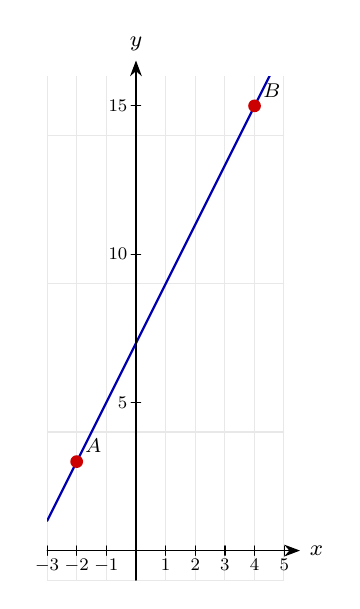
\begin{tikzpicture}[>={Stealth[length=2mm]},font=\footnotesize,line cap=round]
\begin{scope}
\clip (0,0) rectangle (3.012,6.4);
\draw[gray!18] (0,-1.506) grid[xstep=0.376,ystep=1.882] (3.012,6.4);
\draw[blue!70!black,thick] (0,0.753) -- (3.012,6.776);
\end{scope}
\draw[->] (0,0.376) -- (3.212,0.376) node[right]{$x$};
\draw[->] (1.129,0) -- (1.129,6.6) node[above]{$y$};
\draw (0,0.316) -- (0,0.436) node[below=2pt,scale=0.8]{$-3$};
\draw (0.376,0.316) -- (0.376,0.436) node[below=2pt,scale=0.8]{$-2$};
\draw (0.753,0.316) -- (0.753,0.436) node[below=2pt,scale=0.8]{$-1$};
\draw (1.506,0.316) -- (1.506,0.436) node[below=2pt,scale=0.8]{$1$};
\draw (1.882,0.316) -- (1.882,0.436) node[below=2pt,scale=0.8]{$2$};
\draw (2.259,0.316) -- (2.259,0.436) node[below=2pt,scale=0.8]{$3$};
\draw (2.635,0.316) -- (2.635,0.436) node[below=2pt,scale=0.8]{$4$};
\draw (3.012,0.316) -- (3.012,0.436) node[below=2pt,scale=0.8]{$5$};
\draw (1.069,2.259) -- (1.189,2.259) node[left=2pt,scale=0.8]{$5$};
\draw (1.069,4.141) -- (1.189,4.141) node[left=2pt,scale=0.8]{$10$};
\draw (1.069,6.024) -- (1.189,6.024) node[left=2pt,scale=0.8]{$15$};
\fill[red!80!black] (0.376,1.506) circle (2.3pt);
\node[above right,scale=0.9] at (0.376,1.506) {$A$};
\fill[red!80!black] (2.635,6.024) circle (2.3pt);
\node[above right,scale=0.9] at (2.635,6.024) {$B$};
\end{tikzpicture}
}
\end{center}
\small The line(s) and key points shown on the coordinate plane.\normalsize

\medskip\hrule

\section*{Equation of a Straight Line 10\quad\small\texttt{(cg1-010)}}
\addcontentsline{toc}{section}{Equation of a Straight Line 10 (cg1-010)}
\textit{Difficulty: Foundation \quad\textbar\quad Marks: 3}

\question{Find the equation of the line passing through \( (0, -4) \) and \( (5, 6) \). Give your answer in the form \( y = mx + c \).}

\textbf{Worked solution.}

\textit{Step 1: Since one point is \( (0, -4) \), the \( y \)-intercept is \( c = -4 \).}
\[\begin{gathered}
c = -4
\end{gathered}\]
When \( x = 0 \), the point is on the \( y \)-axis, so \( c \) is read directly.

\textit{Step 2: Find the gradient.}
\[\begin{gathered}
m = \dfrac{6 - (-4)}{5 - 0} = \dfrac{10}{5} = 2
\end{gathered}\]
Apply \(m = \frac{y_2 - y_1}{x_2 - x_1}\). Watch the double negative: \(6 - (-4) = 10\), not 2.

\textit{Step 3: Write the equation.}
\[\begin{gathered}
y = 2x - 4
\end{gathered}\]
Combine \(m = 2\) and \(c = -4\) into \(y = mx + c\).

\begin{answerbox}
\textbf{Final answer:}\quad \(\displaystyle y = 2x - 4\)
\end{answerbox}
\textbf{Diagram.}

\begin{center}
\resizebox{\ifdim\width>\linewidth \linewidth\else \width\fi}{!}{%
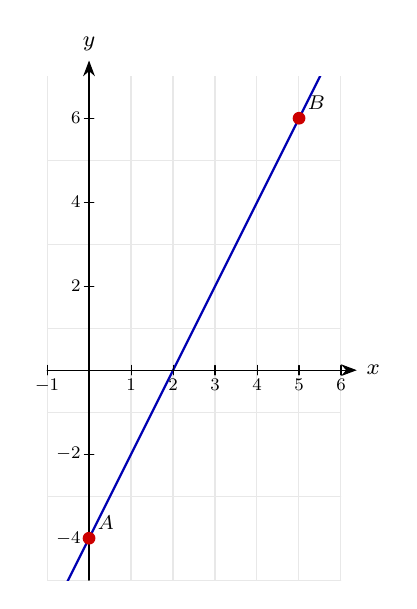
\begin{tikzpicture}[>={Stealth[length=2mm]},font=\footnotesize,line cap=round]
\begin{scope}
\clip (0,0) rectangle (3.733,6.4);
\draw[gray!18] (0,-0.533) grid[xstep=0.533,ystep=1.067] (3.733,6.4);
\draw[blue!70!black,thick] (0,-0.533) -- (3.733,6.933);
\end{scope}
\draw[->] (0,2.667) -- (3.933,2.667) node[right]{$x$};
\draw[->] (0.533,0) -- (0.533,6.6) node[above]{$y$};
\draw (0,2.607) -- (0,2.727) node[below=2pt,scale=0.8]{$-1$};
\draw (1.067,2.607) -- (1.067,2.727) node[below=2pt,scale=0.8]{$1$};
\draw (1.6,2.607) -- (1.6,2.727) node[below=2pt,scale=0.8]{$2$};
\draw (2.133,2.607) -- (2.133,2.727) node[below=2pt,scale=0.8]{$3$};
\draw (2.667,2.607) -- (2.667,2.727) node[below=2pt,scale=0.8]{$4$};
\draw (3.2,2.607) -- (3.2,2.727) node[below=2pt,scale=0.8]{$5$};
\draw (3.733,2.607) -- (3.733,2.727) node[below=2pt,scale=0.8]{$6$};
\draw (0.473,0.533) -- (0.593,0.533) node[left=2pt,scale=0.8]{$-4$};
\draw (0.473,1.6) -- (0.593,1.6) node[left=2pt,scale=0.8]{$-2$};
\draw (0.473,3.733) -- (0.593,3.733) node[left=2pt,scale=0.8]{$2$};
\draw (0.473,4.8) -- (0.593,4.8) node[left=2pt,scale=0.8]{$4$};
\draw (0.473,5.867) -- (0.593,5.867) node[left=2pt,scale=0.8]{$6$};
\fill[red!80!black] (0.533,0.533) circle (2.3pt);
\node[above right,scale=0.9] at (0.533,0.533) {$A$};
\fill[red!80!black] (3.2,5.867) circle (2.3pt);
\node[above right,scale=0.9] at (3.2,5.867) {$B$};
\end{tikzpicture}
}
\end{center}
\small The line(s) and key points shown on the coordinate plane.\normalsize

\medskip\hrule

\section*{Equation of a Straight Line 11\quad\small\texttt{(cg1-011)}}
\addcontentsline{toc}{section}{Equation of a Straight Line 11 (cg1-011)}
\textit{Difficulty: Foundation \quad\textbar\quad Marks: 4}

\question{Find the equation of the line passing through \( (-3, -1) \) and \( (6, 8) \). Give your answer in the form \( y = mx + c \).}

\textbf{Worked solution.}

\textit{Step 1: Find the gradient.}
\[\begin{gathered}
m = \dfrac{8 - (-1)}{6 - (-3)} = \dfrac{9}{9} = 1
\end{gathered}\]
Both differences are 9, giving a gradient of 1.

\textit{Step 2: Use \( y = x + c \) and substitute \( (6, 8) \).}
\[\begin{gathered}
8 = 6 + c \implies c = 2
\end{gathered}\]
Any point on the line satisfies its equation, so substituting the coordinates lets us solve for the unknown intercept \(c\).

\textit{Step 3: Write the equation.}
\[\begin{gathered}
y = x + 2
\end{gathered}\]
Combine \(m = 1\) and \(c = 2\) into \(y = mx + c\).

\begin{answerbox}
\textbf{Final answer:}\quad \(\displaystyle y = x + 2\)
\end{answerbox}
\textbf{Diagram.}

\begin{center}
\resizebox{\ifdim\width>\linewidth \linewidth\else \width\fi}{!}{%
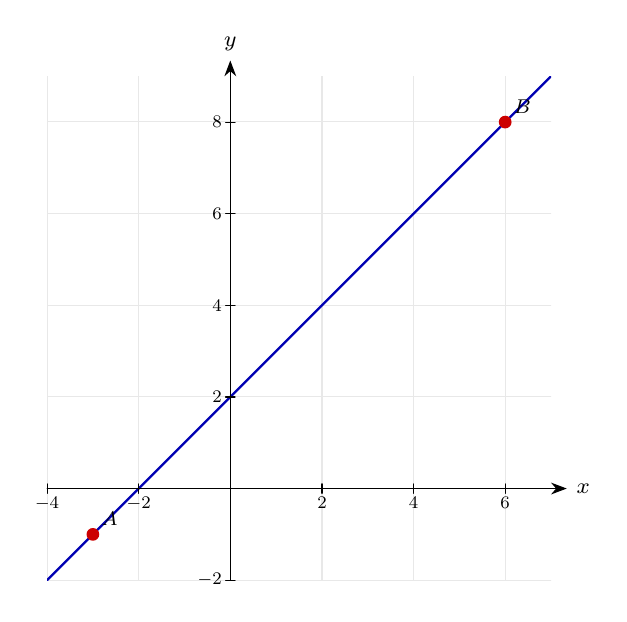
\begin{tikzpicture}[>={Stealth[length=2mm]},font=\footnotesize,line cap=round]
\begin{scope}
\clip (0,0) rectangle (6.4,6.4);
\draw[gray!18] (0,0) grid[xstep=1.164,ystep=1.164] (6.4,6.4);
\draw[blue!70!black,thick] (0,0) -- (6.4,6.4);
\end{scope}
\draw[->] (0,1.164) -- (6.6,1.164) node[right]{$x$};
\draw[->] (2.327,0) -- (2.327,6.6) node[above]{$y$};
\draw (0,1.104) -- (0,1.224) node[below=2pt,scale=0.8]{$-4$};
\draw (1.164,1.104) -- (1.164,1.224) node[below=2pt,scale=0.8]{$-2$};
\draw (3.491,1.104) -- (3.491,1.224) node[below=2pt,scale=0.8]{$2$};
\draw (4.655,1.104) -- (4.655,1.224) node[below=2pt,scale=0.8]{$4$};
\draw (5.818,1.104) -- (5.818,1.224) node[below=2pt,scale=0.8]{$6$};
\draw (2.267,0) -- (2.387,0) node[left=2pt,scale=0.8]{$-2$};
\draw (2.267,2.327) -- (2.387,2.327) node[left=2pt,scale=0.8]{$2$};
\draw (2.267,3.491) -- (2.387,3.491) node[left=2pt,scale=0.8]{$4$};
\draw (2.267,4.655) -- (2.387,4.655) node[left=2pt,scale=0.8]{$6$};
\draw (2.267,5.818) -- (2.387,5.818) node[left=2pt,scale=0.8]{$8$};
\fill[red!80!black] (0.582,0.582) circle (2.3pt);
\node[above right,scale=0.9] at (0.582,0.582) {$A$};
\fill[red!80!black] (5.818,5.818) circle (2.3pt);
\node[above right,scale=0.9] at (5.818,5.818) {$B$};
\end{tikzpicture}
}
\end{center}
\small The line(s) and key points shown on the coordinate plane.\normalsize

\medskip\hrule

\section*{Equation of a Straight Line 12\quad\small\texttt{(cg1-012)}}
\addcontentsline{toc}{section}{Equation of a Straight Line 12 (cg1-012)}
\textit{Difficulty: Foundation \quad\textbar\quad Marks: 4}

\question{Find the equation of the line passing through \( (-5, 11) \) and \( (3, -5) \). Give your answer in the form \( y = mx + c \).}

\textbf{Worked solution.}

\textit{Step 1: Find the gradient.}
\[\begin{gathered}
m = \dfrac{-5 - 11}{3 - (-5)} = \dfrac{-16}{8} = -2
\end{gathered}\]
The line has a negative gradient --- it slopes downward left to right.

\textit{Step 2: Use \( y = -2x + c \) and substitute \( (3, -5) \).}
\[\begin{gathered}
-5 = -2(3) + c \implies -5 = -6 + c \implies c = 1
\end{gathered}\]
You can substitute either point to find \( c \) --- both give the same result.

\textit{Step 3: Write the equation.}
\[\begin{gathered}
y = -2x + 1
\end{gathered}\]
Combine \(m = -2\) and \(c = 1\) into \(y = mx + c\).

\begin{answerbox}
\textbf{Final answer:}\quad \(\displaystyle y = -2x + 1\)
\end{answerbox}
\textbf{Common mistake.} Either point can be substituted to find \(c\). Using \((-5, 11)\): \(11 = -2(-5) + c \implies c = 1\) gives the same answer.

\textbf{Diagram.}

\begin{center}
\resizebox{\ifdim\width>\linewidth \linewidth\else \width\fi}{!}{%
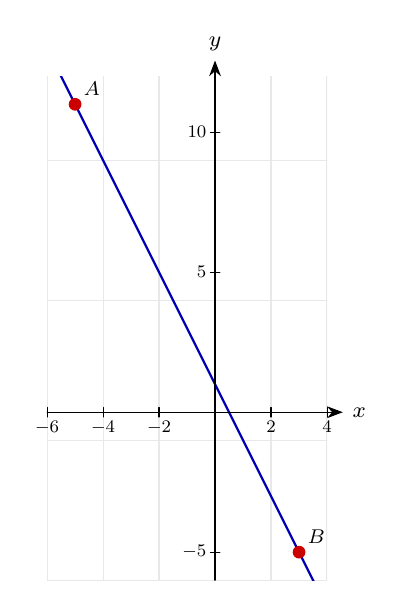
\begin{tikzpicture}[>={Stealth[length=2mm]},font=\footnotesize,line cap=round]
\begin{scope}
\clip (0,0) rectangle (3.556,6.4);
\draw[gray!18] (0,-1.422) grid[xstep=0.711,ystep=1.778] (3.556,6.4);
\draw[blue!70!black,thick] (0,6.756) -- (3.556,-0.356);
\end{scope}
\draw[->] (0,2.133) -- (3.756,2.133) node[right]{$x$};
\draw[->] (2.133,0) -- (2.133,6.6) node[above]{$y$};
\draw (0,2.073) -- (0,2.193) node[below=2pt,scale=0.8]{$-6$};
\draw (0.711,2.073) -- (0.711,2.193) node[below=2pt,scale=0.8]{$-4$};
\draw (1.422,2.073) -- (1.422,2.193) node[below=2pt,scale=0.8]{$-2$};
\draw (2.844,2.073) -- (2.844,2.193) node[below=2pt,scale=0.8]{$2$};
\draw (3.556,2.073) -- (3.556,2.193) node[below=2pt,scale=0.8]{$4$};
\draw (2.073,0.356) -- (2.193,0.356) node[left=2pt,scale=0.8]{$-5$};
\draw (2.073,3.911) -- (2.193,3.911) node[left=2pt,scale=0.8]{$5$};
\draw (2.073,5.689) -- (2.193,5.689) node[left=2pt,scale=0.8]{$10$};
\fill[red!80!black] (0.356,6.044) circle (2.3pt);
\node[above right,scale=0.9] at (0.356,6.044) {$A$};
\fill[red!80!black] (3.2,0.356) circle (2.3pt);
\node[above right,scale=0.9] at (3.2,0.356) {$B$};
\end{tikzpicture}
}
\end{center}
\small The line(s) and key points shown on the coordinate plane.\normalsize

\medskip\hrule

\section*{Equation of a Straight Line 13\quad\small\texttt{(cg1-013)}}
\addcontentsline{toc}{section}{Equation of a Straight Line 13 (cg1-013)}
\textit{Difficulty: Foundation \quad\textbar\quad Marks: 2}

\question{Write the equation \( y = 3x - 4 \) in the form \( ax + by + c = 0 \), where \( a \), \( b \) and \( c \) are integers.}

\textbf{Worked solution.}

\textit{Move all terms to one side.}
\[\begin{gathered}
y = 3x - 4 \quad\quad \Rightarrow \quad\quad y - 3x + 4 = 0
\end{gathered}\]
Move all terms to one side. Multiplying through by \(-1\) gives the equivalent form \(3x - y - 4 = 0\).

\begin{answerbox}
\textbf{Final answer:}\quad \(\displaystyle y - 3x + 4 = 0\), or equivalently \(\displaystyle 3x - y - 4 = 0\)
\end{answerbox}
\textbf{Common mistake.} Both forms are equally valid. Multiplying through by \(-1\) gives the other form. Convention is usually to make the \(x\) coefficient positive, but both are correct.

\textbf{Diagram.}

\begin{center}
\resizebox{\ifdim\width>\linewidth \linewidth\else \width\fi}{!}{%
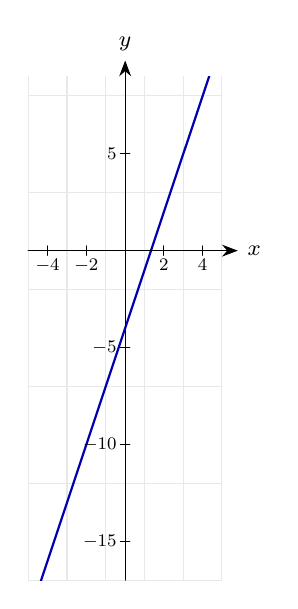
\begin{tikzpicture}[>={Stealth[length=2mm]},font=\footnotesize,line cap=round]
\begin{scope}
\clip (0,0) rectangle (2.462,6.4);
\draw[gray!18] (-0.246,-0.738) grid[xstep=0.492,ystep=1.231] (2.462,6.4);
\draw[blue!70!black,thick] (0,-0.492) -- (2.462,6.892);
\end{scope}
\draw[->] (0,4.185) -- (2.662,4.185) node[right]{$x$};
\draw[->] (1.231,0) -- (1.231,6.6) node[above]{$y$};
\draw (0.246,4.125) -- (0.246,4.245) node[below=2pt,scale=0.8]{$-4$};
\draw (0.738,4.125) -- (0.738,4.245) node[below=2pt,scale=0.8]{$-2$};
\draw (1.723,4.125) -- (1.723,4.245) node[below=2pt,scale=0.8]{$2$};
\draw (2.215,4.125) -- (2.215,4.245) node[below=2pt,scale=0.8]{$4$};
\draw (1.171,0.492) -- (1.291,0.492) node[left=2pt,scale=0.8]{$-15$};
\draw (1.171,1.723) -- (1.291,1.723) node[left=2pt,scale=0.8]{$-10$};
\draw (1.171,2.954) -- (1.291,2.954) node[left=2pt,scale=0.8]{$-5$};
\draw (1.171,5.415) -- (1.291,5.415) node[left=2pt,scale=0.8]{$5$};
\end{tikzpicture}
}
\end{center}
\small The line(s) and key points shown on the coordinate plane.\normalsize

\medskip\hrule

\section*{Equation of a Straight Line 14\quad\small\texttt{(cg1-014)}}
\addcontentsline{toc}{section}{Equation of a Straight Line 14 (cg1-014)}
\textit{Difficulty: Foundation \quad\textbar\quad Marks: 3}

\question{Write the equation \( y = \dfrac{1}{2}x + 3 \) in the form \( ax + by + c = 0 \), where \( a \), \( b \) and \( c \) are integers.}

\textbf{Worked solution.}

\textit{Multiply by 2 to clear the fraction, then rearrange.}
\[\begin{gathered}
y = \dfrac{1}{2}x + 3 \quad\quad \Rightarrow \quad\quad 2y = x + 6 \quad\quad \Rightarrow \quad\quad x - 2y + 6 = 0
\end{gathered}\]
Multiply through by 2 first, then move all terms to one side.

\begin{answerbox}
\textbf{Final answer:}\quad \(\displaystyle x - 2y + 6 = 0\) or equivalently \(\displaystyle -x + 2y - 6 = 0\)
\end{answerbox}
\textbf{Common mistake.} Both forms are equally valid. Multiplying through by \(-1\) gives the other form.

\textbf{Diagram.}

\begin{center}
\resizebox{\ifdim\width>\linewidth \linewidth\else \width\fi}{!}{%
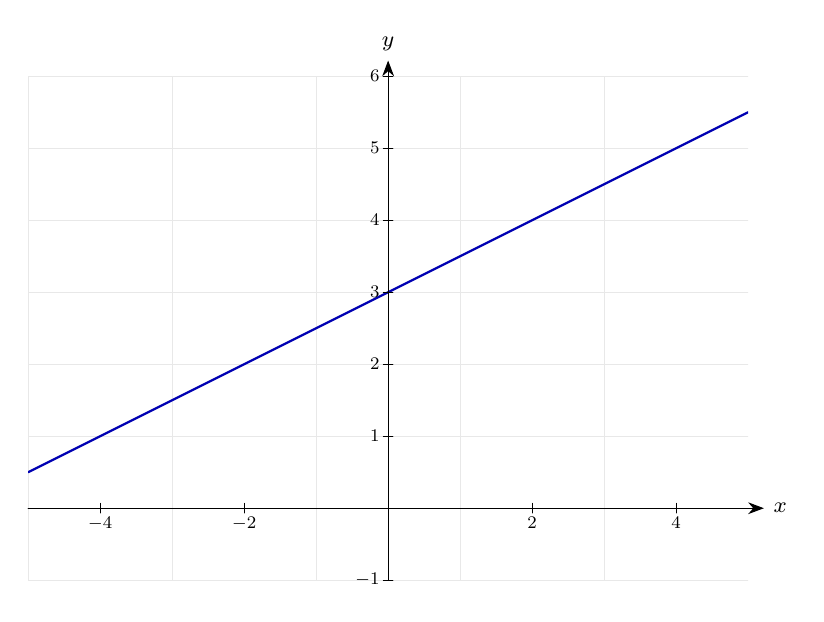
\begin{tikzpicture}[>={Stealth[length=2mm]},font=\footnotesize,line cap=round]
\begin{scope}
\clip (0,0) rectangle (9.143,6.4);
\draw[gray!18] (-0.914,0) grid[xstep=1.829,ystep=0.914] (9.143,6.4);
\draw[blue!70!black,thick] (0,1.371) -- (9.143,5.943);
\end{scope}
\draw[->] (0,0.914) -- (9.343,0.914) node[right]{$x$};
\draw[->] (4.571,0) -- (4.571,6.6) node[above]{$y$};
\draw (0.914,0.854) -- (0.914,0.974) node[below=2pt,scale=0.8]{$-4$};
\draw (2.743,0.854) -- (2.743,0.974) node[below=2pt,scale=0.8]{$-2$};
\draw (6.4,0.854) -- (6.4,0.974) node[below=2pt,scale=0.8]{$2$};
\draw (8.229,0.854) -- (8.229,0.974) node[below=2pt,scale=0.8]{$4$};
\draw (4.511,0) -- (4.631,0) node[left=2pt,scale=0.8]{$-1$};
\draw (4.511,1.829) -- (4.631,1.829) node[left=2pt,scale=0.8]{$1$};
\draw (4.511,2.743) -- (4.631,2.743) node[left=2pt,scale=0.8]{$2$};
\draw (4.511,3.657) -- (4.631,3.657) node[left=2pt,scale=0.8]{$3$};
\draw (4.511,4.571) -- (4.631,4.571) node[left=2pt,scale=0.8]{$4$};
\draw (4.511,5.486) -- (4.631,5.486) node[left=2pt,scale=0.8]{$5$};
\draw (4.511,6.4) -- (4.631,6.4) node[left=2pt,scale=0.8]{$6$};
\end{tikzpicture}
}
\end{center}
\small The line(s) and key points shown on the coordinate plane.\normalsize

\medskip\hrule

\section*{Equation of a Straight Line 15\quad\small\texttt{(cg1-015)}}
\addcontentsline{toc}{section}{Equation of a Straight Line 15 (cg1-015)}
\textit{Difficulty: Foundation \quad\textbar\quad Marks: 4}

\question{Find the equation of the line that passes through the point \( (3, -8) \) and has gradient \( -\dfrac{5}{2} \). Give your answer in the form \( ax + by + c = 0 \), where \( a \), \( b \) and \( c \) are integers.}

\textbf{Worked solution.}

\textit{Find the equation and rearrange.}
\[\begin{gathered}
y + 8 = -\dfrac{5}{2}(x - 3) \quad\quad \Rightarrow \quad\quad 2y + 16 = -5x + 15 \quad\quad \Rightarrow \quad\quad 5x + 2y + 1 = 0
\end{gathered}\]
Substitute into \(y - y_1 = m(x - x_1)\), multiply by 2 to clear the fraction, then collect all terms on one side.

\begin{answerbox}
\textbf{Final answer:}\quad \(\displaystyle 5x + 2y + 1 = 0\) or equivalently \(\displaystyle -5x - 2y - 1 = 0\)
\end{answerbox}
\textbf{Common mistake.} Both forms are equally valid. Multiplying through by \(-1\) gives the other form.

\textbf{Diagram.}

\begin{center}
\resizebox{\ifdim\width>\linewidth \linewidth\else \width\fi}{!}{%
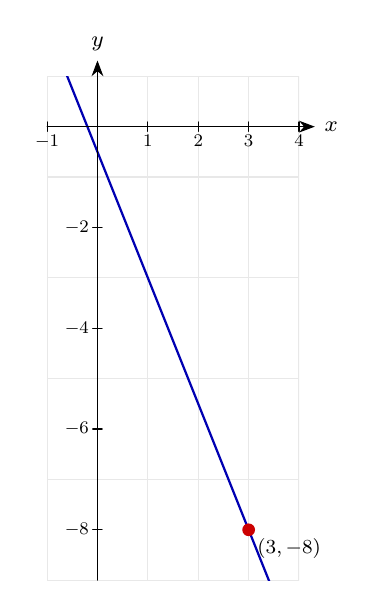
\begin{tikzpicture}[>={Stealth[length=2mm]},font=\footnotesize,line cap=round]
\begin{scope}
\clip (0,0) rectangle (3.2,6.4);
\draw[gray!18] (0,-0.64) grid[xstep=0.64,ystep=1.28] (3.2,6.4);
\draw[blue!70!black,thick] (0,7.04) -- (3.2,-0.96);
\end{scope}
\draw[->] (0,5.76) -- (3.4,5.76) node[right]{$x$};
\draw[->] (0.64,0) -- (0.64,6.6) node[above]{$y$};
\draw (0,5.7) -- (0,5.82) node[below=2pt,scale=0.8]{$-1$};
\draw (1.28,5.7) -- (1.28,5.82) node[below=2pt,scale=0.8]{$1$};
\draw (1.92,5.7) -- (1.92,5.82) node[below=2pt,scale=0.8]{$2$};
\draw (2.56,5.7) -- (2.56,5.82) node[below=2pt,scale=0.8]{$3$};
\draw (3.2,5.7) -- (3.2,5.82) node[below=2pt,scale=0.8]{$4$};
\draw (0.58,0.64) -- (0.7,0.64) node[left=2pt,scale=0.8]{$-8$};
\draw (0.58,1.92) -- (0.7,1.92) node[left=2pt,scale=0.8]{$-6$};
\draw (0.58,3.2) -- (0.7,3.2) node[left=2pt,scale=0.8]{$-4$};
\draw (0.58,4.48) -- (0.7,4.48) node[left=2pt,scale=0.8]{$-2$};
\fill[red!80!black] (2.56,0.64) circle (2.3pt);
\node[below right,scale=0.9] at (2.56,0.64) {$(3,-8)$};
\end{tikzpicture}
}
\end{center}
\small The line(s) and key points shown on the coordinate plane.\normalsize

\medskip\hrule

\section*{Equation of a Straight Line 16\quad\small\texttt{(cg1-016)}}
\addcontentsline{toc}{section}{Equation of a Straight Line 16 (cg1-016)}
\textit{Difficulty: Foundation \quad\textbar\quad Marks: 3}

\question{Write the equation \( 4y - 2x + 8 = 0 \) in the form \( y = mx + c \). State the gradient and \( y \)-intercept.}

\textbf{Worked solution.}

\textit{Step 1: Add \( 2x \) to both sides and subtract 8.}
\[\begin{gathered}
4y = 2x - 8
\end{gathered}\]
Isolate the \(4y\) term so we can divide through to make \(y\) the subject.

\textit{Step 2: Divide every term by 4.}
\[\begin{gathered}
y = \dfrac{1}{2}x - 2
\end{gathered}\]
The equation is now in \( y = mx + c \) form.

\begin{answerbox}
\textbf{Final answer:}\quad \(\displaystyle y = \dfrac{1}{2}x - 2\); gradient = \(\displaystyle \dfrac{1}{2}\), y-intercept = \(\displaystyle (0, -2)\)
\end{answerbox}
\textbf{Diagram.}

\begin{center}
\resizebox{\ifdim\width>\linewidth \linewidth\else \width\fi}{!}{%
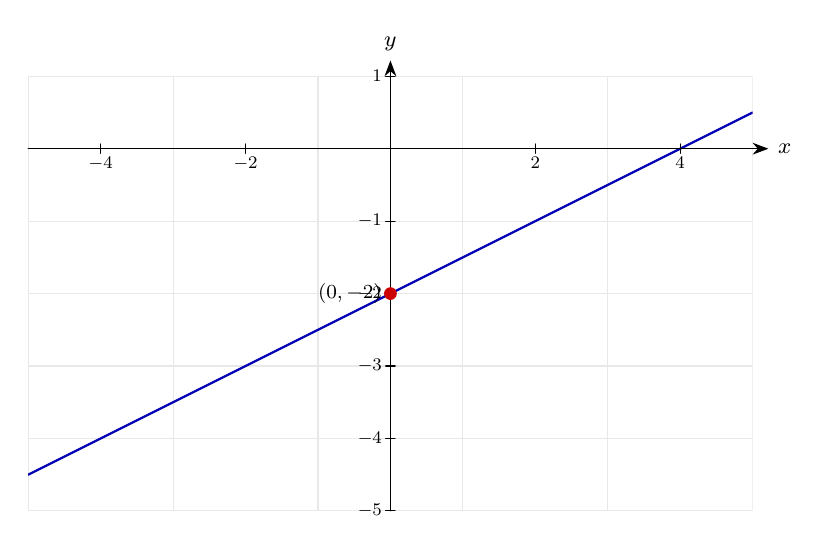
\begin{tikzpicture}[>={Stealth[length=2mm]},font=\footnotesize,line cap=round]
\begin{scope}
\clip (0,0) rectangle (9.2,5.52);
\draw[gray!18] (-0.92,0) grid[xstep=1.84,ystep=0.92] (9.2,5.52);
\draw[blue!70!black,thick] (0,0.46) -- (9.2,5.06);
\end{scope}
\draw[->] (0,4.6) -- (9.4,4.6) node[right]{$x$};
\draw[->] (4.6,0) -- (4.6,5.72) node[above]{$y$};
\draw (0.92,4.54) -- (0.92,4.66) node[below=2pt,scale=0.8]{$-4$};
\draw (2.76,4.54) -- (2.76,4.66) node[below=2pt,scale=0.8]{$-2$};
\draw (6.44,4.54) -- (6.44,4.66) node[below=2pt,scale=0.8]{$2$};
\draw (8.28,4.54) -- (8.28,4.66) node[below=2pt,scale=0.8]{$4$};
\draw (4.54,0) -- (4.66,0) node[left=2pt,scale=0.8]{$-5$};
\draw (4.54,0.92) -- (4.66,0.92) node[left=2pt,scale=0.8]{$-4$};
\draw (4.54,1.84) -- (4.66,1.84) node[left=2pt,scale=0.8]{$-3$};
\draw (4.54,2.76) -- (4.66,2.76) node[left=2pt,scale=0.8]{$-2$};
\draw (4.54,3.68) -- (4.66,3.68) node[left=2pt,scale=0.8]{$-1$};
\draw (4.54,5.52) -- (4.66,5.52) node[left=2pt,scale=0.8]{$1$};
\fill[red!80!black] (4.6,2.76) circle (2.3pt);
\node[left,scale=0.9] at (4.6,2.76) {$(0,-2)$};
\end{tikzpicture}
}
\end{center}
\small The line(s) and key points shown on the coordinate plane.\normalsize

\medskip\hrule

\section*{Equation of a Straight Line 17\quad\small\texttt{(cg1-017)}}
\addcontentsline{toc}{section}{Equation of a Straight Line 17 (cg1-017)}
\textit{Difficulty: Foundation \quad\textbar\quad Marks: 3}

\question{Find the gradient and \( y \)-intercept of the line \( 3x + 6y - 12 = 0 \).}

\textbf{Worked solution.}

\textit{Rearrange to make \( y \) the subject.}
\[\begin{gathered}
6y = -3x + 12 \implies y = -\dfrac{1}{2}x + 2
\end{gathered}\]
Subtract \(3x\), add 12 to both sides, then divide by 6.

\begin{answerbox}
\textbf{Final answer:}\quad Gradient = \(\displaystyle -\dfrac{1}{2}\), y-intercept = \(\displaystyle (0, 2)\)
\end{answerbox}
\textbf{Diagram.}

\begin{center}
\resizebox{\ifdim\width>\linewidth \linewidth\else \width\fi}{!}{%
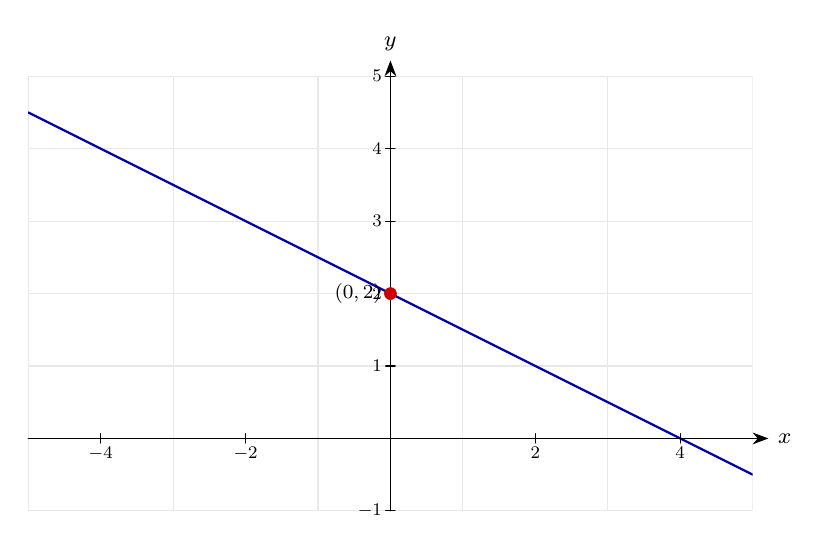
\begin{tikzpicture}[>={Stealth[length=2mm]},font=\footnotesize,line cap=round]
\begin{scope}
\clip (0,0) rectangle (9.2,5.52);
\draw[gray!18] (-0.92,0) grid[xstep=1.84,ystep=0.92] (9.2,5.52);
\draw[blue!70!black,thick] (0,5.06) -- (9.2,0.46);
\end{scope}
\draw[->] (0,0.92) -- (9.4,0.92) node[right]{$x$};
\draw[->] (4.6,0) -- (4.6,5.72) node[above]{$y$};
\draw (0.92,0.86) -- (0.92,0.98) node[below=2pt,scale=0.8]{$-4$};
\draw (2.76,0.86) -- (2.76,0.98) node[below=2pt,scale=0.8]{$-2$};
\draw (6.44,0.86) -- (6.44,0.98) node[below=2pt,scale=0.8]{$2$};
\draw (8.28,0.86) -- (8.28,0.98) node[below=2pt,scale=0.8]{$4$};
\draw (4.54,0) -- (4.66,0) node[left=2pt,scale=0.8]{$-1$};
\draw (4.54,1.84) -- (4.66,1.84) node[left=2pt,scale=0.8]{$1$};
\draw (4.54,2.76) -- (4.66,2.76) node[left=2pt,scale=0.8]{$2$};
\draw (4.54,3.68) -- (4.66,3.68) node[left=2pt,scale=0.8]{$3$};
\draw (4.54,4.6) -- (4.66,4.6) node[left=2pt,scale=0.8]{$4$};
\draw (4.54,5.52) -- (4.66,5.52) node[left=2pt,scale=0.8]{$5$};
\fill[red!80!black] (4.6,2.76) circle (2.3pt);
\node[left,scale=0.9] at (4.6,2.76) {$(0,2)$};
\end{tikzpicture}
}
\end{center}
\small The line(s) and key points shown on the coordinate plane.\normalsize

\medskip\hrule

\section*{Equation of a Straight Line 18\quad\small\texttt{(cg1-018)}}
\addcontentsline{toc}{section}{Equation of a Straight Line 18 (cg1-018)}
\textit{Difficulty: Foundation \quad\textbar\quad Marks: 3}

\question{Find the equation of the straight line that passes through the point \( (5, 3) \) and has gradient \( 2 \). Give your answer in the form \( y = mx + c \).}

\textbf{Worked solution.}

\textit{Step 1: Write \( y = 2x + c \) and substitute \( (5, 3) \).}
\[\begin{gathered}
3 = 2(5) + c \implies 3 = 10 + c \implies c = -7
\end{gathered}\]
Substituting the given point allows us to find \( c \).

\textit{Step 2: Write the final equation.}
\[\begin{gathered}
y = 2x - 7
\end{gathered}\]
Slot \(m = 2\) and \(c = -7\) back into \(y = mx + c\).

\begin{answerbox}
\textbf{Final answer:}\quad \(\displaystyle y = 2x - 7\)
\end{answerbox}
\textbf{Diagram.}

\begin{center}
\resizebox{\ifdim\width>\linewidth \linewidth\else \width\fi}{!}{%
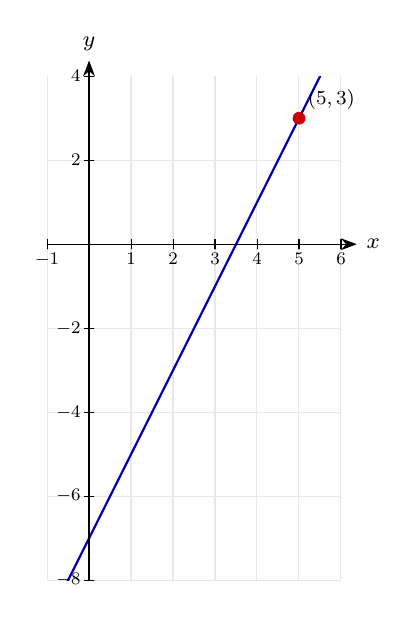
\begin{tikzpicture}[>={Stealth[length=2mm]},font=\footnotesize,line cap=round]
\begin{scope}
\clip (0,0) rectangle (3.733,6.4);
\draw[gray!18] (0,0) grid[xstep=0.533,ystep=1.067] (3.733,6.4);
\draw[blue!70!black,thick] (0,-0.533) -- (3.733,6.933);
\end{scope}
\draw[->] (0,4.267) -- (3.933,4.267) node[right]{$x$};
\draw[->] (0.533,0) -- (0.533,6.6) node[above]{$y$};
\draw (0,4.207) -- (0,4.327) node[below=2pt,scale=0.8]{$-1$};
\draw (1.067,4.207) -- (1.067,4.327) node[below=2pt,scale=0.8]{$1$};
\draw (1.6,4.207) -- (1.6,4.327) node[below=2pt,scale=0.8]{$2$};
\draw (2.133,4.207) -- (2.133,4.327) node[below=2pt,scale=0.8]{$3$};
\draw (2.667,4.207) -- (2.667,4.327) node[below=2pt,scale=0.8]{$4$};
\draw (3.2,4.207) -- (3.2,4.327) node[below=2pt,scale=0.8]{$5$};
\draw (3.733,4.207) -- (3.733,4.327) node[below=2pt,scale=0.8]{$6$};
\draw (0.473,0) -- (0.593,0) node[left=2pt,scale=0.8]{$-8$};
\draw (0.473,1.067) -- (0.593,1.067) node[left=2pt,scale=0.8]{$-6$};
\draw (0.473,2.133) -- (0.593,2.133) node[left=2pt,scale=0.8]{$-4$};
\draw (0.473,3.2) -- (0.593,3.2) node[left=2pt,scale=0.8]{$-2$};
\draw (0.473,5.333) -- (0.593,5.333) node[left=2pt,scale=0.8]{$2$};
\draw (0.473,6.4) -- (0.593,6.4) node[left=2pt,scale=0.8]{$4$};
\fill[red!80!black] (3.2,5.867) circle (2.3pt);
\node[above right,scale=0.9] at (3.2,5.867) {$(5,3)$};
\end{tikzpicture}
}
\end{center}
\small The line(s) and key points shown on the coordinate plane.\normalsize

\medskip\hrule

\section*{Equation of a Straight Line 19\quad\small\texttt{(cg1-019)}}
\addcontentsline{toc}{section}{Equation of a Straight Line 19 (cg1-019)}
\textit{Difficulty: Foundation \quad\textbar\quad Marks: 3}

\question{Find the equation of the straight line with gradient \( -3 \) passing through \( (2, 4) \). Give your answer in the form \( y = mx + c \).}

\textbf{Worked solution.}

\textit{Step 1: Write \( y = -3x + c \) and substitute \( (2, 4) \).}
\[\begin{gathered}
4 = -3(2) + c \implies 4 = -6 + c \implies c = 10
\end{gathered}\]
The point lies on the line, so its coordinates must satisfy the equation. Adding 6 to both sides gives \(c\).

\textit{Step 2: Write the final equation.}
\[\begin{gathered}
y = -3x + 10
\end{gathered}\]
Combine \(m = -3\) and \(c = 10\) into \(y = mx + c\).

\begin{answerbox}
\textbf{Final answer:}\quad \(\displaystyle y = -3x + 10\)
\end{answerbox}
\textbf{Diagram.}

\begin{center}
\resizebox{\ifdim\width>\linewidth \linewidth\else \width\fi}{!}{%
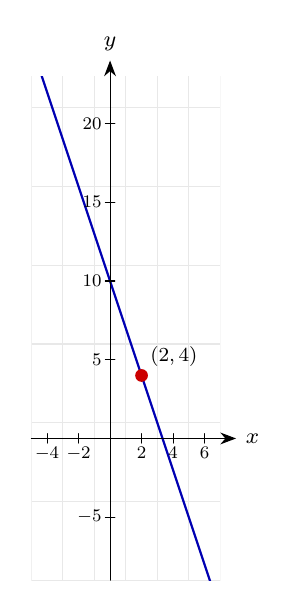
\begin{tikzpicture}[>={Stealth[length=2mm]},font=\footnotesize,line cap=round]
\begin{scope}
\clip (0,0) rectangle (2.4,6.4);
\draw[gray!18] (-0.2,-0.2) grid[xstep=0.4,ystep=1] (2.4,6.4);
\draw[blue!70!black,thick] (0,6.8) -- (2.4,-0.4);
\end{scope}
\draw[->] (0,1.8) -- (2.6,1.8) node[right]{$x$};
\draw[->] (1,0) -- (1,6.6) node[above]{$y$};
\draw (0.2,1.74) -- (0.2,1.86) node[below=2pt,scale=0.8]{$-4$};
\draw (0.6,1.74) -- (0.6,1.86) node[below=2pt,scale=0.8]{$-2$};
\draw (1.4,1.74) -- (1.4,1.86) node[below=2pt,scale=0.8]{$2$};
\draw (1.8,1.74) -- (1.8,1.86) node[below=2pt,scale=0.8]{$4$};
\draw (2.2,1.74) -- (2.2,1.86) node[below=2pt,scale=0.8]{$6$};
\draw (0.94,0.8) -- (1.06,0.8) node[left=2pt,scale=0.8]{$-5$};
\draw (0.94,2.8) -- (1.06,2.8) node[left=2pt,scale=0.8]{$5$};
\draw (0.94,3.8) -- (1.06,3.8) node[left=2pt,scale=0.8]{$10$};
\draw (0.94,4.8) -- (1.06,4.8) node[left=2pt,scale=0.8]{$15$};
\draw (0.94,5.8) -- (1.06,5.8) node[left=2pt,scale=0.8]{$20$};
\fill[red!80!black] (1.4,2.6) circle (2.3pt);
\node[above right,scale=0.9] at (1.4,2.6) {$(2,4)$};
\end{tikzpicture}
}
\end{center}
\small The line(s) and key points shown on the coordinate plane.\normalsize

\medskip\hrule

\section*{Equation of a Straight Line 20\quad\small\texttt{(cg1-020)}}
\addcontentsline{toc}{section}{Equation of a Straight Line 20 (cg1-020)}
\textit{Difficulty: Foundation \quad\textbar\quad Marks: 4}

\question{Find the equation of the straight line with gradient \( \dfrac{3}{4} \) passing through \( (-4, 1) \). Give your answer in the form \( y = mx + c \).}

\textbf{Worked solution.}

\textit{Step 1: Write \( y = \frac{3}{4}x + c \) and substitute \( (-4, 1) \).}
\[\begin{gathered}
1 = \dfrac{3}{4}(-4) + c \implies 1 = -3 + c \implies c = 4
\end{gathered}\]
Be careful with the negative \( x \)-value.

\textit{Step 2: Write the final equation.}
\[\begin{gathered}
y = \dfrac{3}{4}x + 4
\end{gathered}\]
Slot \(m = \tfrac{3}{4}\) and \(c = 4\) into \(y = mx + c\).

\begin{answerbox}
\textbf{Final answer:}\quad \(\displaystyle y = \dfrac{3}{4}x + 4\)
\end{answerbox}
\textbf{Diagram.}

\begin{center}
\resizebox{\ifdim\width>\linewidth \linewidth\else \width\fi}{!}{%
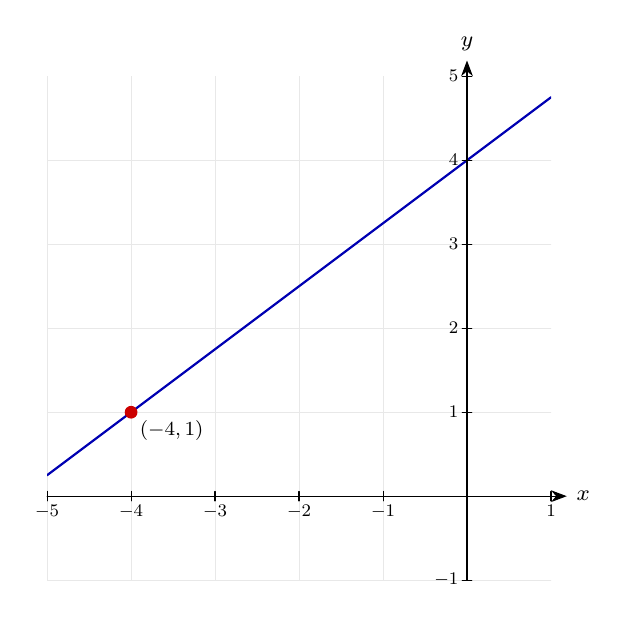
\begin{tikzpicture}[>={Stealth[length=2mm]},font=\footnotesize,line cap=round]
\begin{scope}
\clip (0,0) rectangle (6.4,6.4);
\draw[gray!18] (0,0) grid[xstep=1.067,ystep=1.067] (6.4,6.4);
\draw[blue!70!black,thick] (0,1.333) -- (6.4,6.133);
\end{scope}
\draw[->] (0,1.067) -- (6.6,1.067) node[right]{$x$};
\draw[->] (5.333,0) -- (5.333,6.6) node[above]{$y$};
\draw (0,1.007) -- (0,1.127) node[below=2pt,scale=0.8]{$-5$};
\draw (1.067,1.007) -- (1.067,1.127) node[below=2pt,scale=0.8]{$-4$};
\draw (2.133,1.007) -- (2.133,1.127) node[below=2pt,scale=0.8]{$-3$};
\draw (3.2,1.007) -- (3.2,1.127) node[below=2pt,scale=0.8]{$-2$};
\draw (4.267,1.007) -- (4.267,1.127) node[below=2pt,scale=0.8]{$-1$};
\draw (6.4,1.007) -- (6.4,1.127) node[below=2pt,scale=0.8]{$1$};
\draw (5.273,0) -- (5.393,0) node[left=2pt,scale=0.8]{$-1$};
\draw (5.273,2.133) -- (5.393,2.133) node[left=2pt,scale=0.8]{$1$};
\draw (5.273,3.2) -- (5.393,3.2) node[left=2pt,scale=0.8]{$2$};
\draw (5.273,4.267) -- (5.393,4.267) node[left=2pt,scale=0.8]{$3$};
\draw (5.273,5.333) -- (5.393,5.333) node[left=2pt,scale=0.8]{$4$};
\draw (5.273,6.4) -- (5.393,6.4) node[left=2pt,scale=0.8]{$5$};
\fill[red!80!black] (1.067,2.133) circle (2.3pt);
\node[below right,scale=0.9] at (1.067,2.133) {$(-4,1)$};
\end{tikzpicture}
}
\end{center}
\small The line(s) and key points shown on the coordinate plane.\normalsize

\medskip\hrule

\section*{Equation of a Straight Line 21\quad\small\texttt{(cg1-021)}}
\addcontentsline{toc}{section}{Equation of a Straight Line 21 (cg1-021)}
\textit{Difficulty: Foundation \quad\textbar\quad Marks: 2}

\question{A straight line has equation \( y = 5x - 3 \). State whether or not the point \( (2, 7) \) lies on the line. Show your working.}

\textbf{Worked solution.}

\textit{Step 1: Substitute \( x = 2 \) into the equation.}
\[\begin{gathered}
y = 5(2) - 3 = 10 - 3 = 7
\end{gathered}\]
The calculated \( y \)-value matches the given \( y \)-coordinate.

\textit{Step 2: State the conclusion.}
\[\begin{gathered}
7 = 7 \implies (2, 7) \text{ lies on the line.}
\end{gathered}\]
A point lies on a line if and only if its coordinates satisfy the equation. Since the calculated \(y\) equals the given \(y\), the point is on the line.

\begin{answerbox}
\textbf{Final answer:}\quad Yes, \(\displaystyle (2, 7)\) lies on the line.
\end{answerbox}
\textbf{Diagram.}

\begin{center}
\resizebox{\ifdim\width>\linewidth \linewidth\else \width\fi}{!}{%
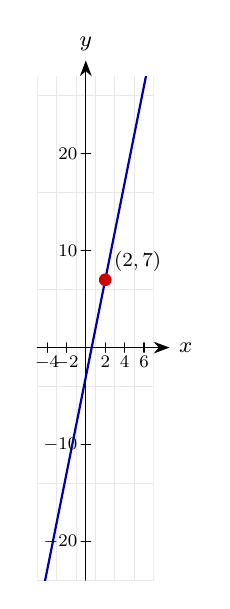
\begin{tikzpicture}[>={Stealth[length=2mm]},font=\footnotesize,line cap=round]
\begin{scope}
\clip (0,0) rectangle (1.477,6.4);
\draw[gray!18] (-0.123,-0.738) grid[xstep=0.246,ystep=1.231] (1.477,6.4);
\draw[blue!70!black,thick] (0,-0.492) -- (1.477,6.892);
\end{scope}
\draw[->] (0,2.954) -- (1.677,2.954) node[right]{$x$};
\draw[->] (0.615,0) -- (0.615,6.6) node[above]{$y$};
\draw (0.123,2.894) -- (0.123,3.014) node[below=2pt,scale=0.8]{$-4$};
\draw (0.369,2.894) -- (0.369,3.014) node[below=2pt,scale=0.8]{$-2$};
\draw (0.862,2.894) -- (0.862,3.014) node[below=2pt,scale=0.8]{$2$};
\draw (1.108,2.894) -- (1.108,3.014) node[below=2pt,scale=0.8]{$4$};
\draw (1.354,2.894) -- (1.354,3.014) node[below=2pt,scale=0.8]{$6$};
\draw (0.555,0.492) -- (0.675,0.492) node[left=2pt,scale=0.8]{$-20$};
\draw (0.555,1.723) -- (0.675,1.723) node[left=2pt,scale=0.8]{$-10$};
\draw (0.555,4.185) -- (0.675,4.185) node[left=2pt,scale=0.8]{$10$};
\draw (0.555,5.415) -- (0.675,5.415) node[left=2pt,scale=0.8]{$20$};
\fill[red!80!black] (0.862,3.815) circle (2.3pt);
\node[above right,scale=0.9] at (0.862,3.815) {$(2,7)$};
\end{tikzpicture}
}
\end{center}
\small The line(s) and key points shown on the coordinate plane.\normalsize

\medskip\hrule

\section*{Equation of a Straight Line 22\quad\small\texttt{(cg1-022)}}
\addcontentsline{toc}{section}{Equation of a Straight Line 22 (cg1-022)}
\textit{Difficulty: Foundation \quad\textbar\quad Marks: 4}

\question{A line passes through the points \( (1, 3) \) and \( (4, 9) \). Does the point \( (10, 21) \) also lie on the line? Show full working.}

\textbf{Worked solution.}

\textit{Step 1: Find the gradient of the line.}
\[\begin{gathered}
m = \dfrac{9 - 3}{4 - 1} = \dfrac{6}{3} = 2
\end{gathered}\]
Apply \(m = \frac{y_2 - y_1}{x_2 - x_1}\) using the two given points.

\textit{Step 2: Find the equation: use \( y = 2x + c \) with \( (1, 3) \).}
\[\begin{gathered}
3 = 2(1) + c \implies c = 1 \implies y = 2x + 1
\end{gathered}\]
Substitute either point into \(y = mx + c\) and solve for \(c\) --- the line equation is then fully determined.

\textit{Step 3: Test \( (10, 21) \).}
\[\begin{gathered}
2(10) + 1 = 21 \checkmark
\end{gathered}\]
The point satisfies the equation.

\begin{answerbox}
\textbf{Final answer:}\quad Yes, \(\displaystyle (10, 21)\) lies on the line.
\end{answerbox}
\textbf{Diagram.}

\begin{center}
\resizebox{\ifdim\width>\linewidth \linewidth\else \width\fi}{!}{%
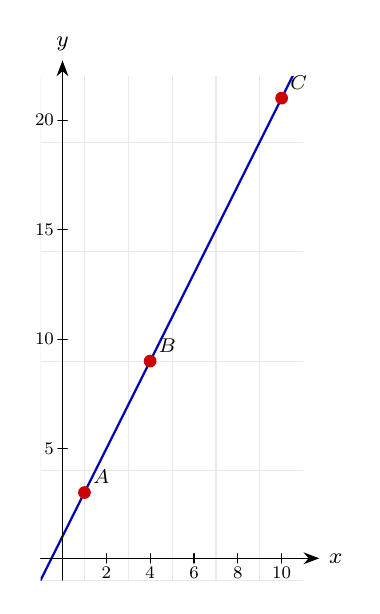
\begin{tikzpicture}[>={Stealth[length=2mm]},font=\footnotesize,line cap=round]
\begin{scope}
\clip (0,0) rectangle (3.339,6.4);
\draw[gray!18] (-0.278,-1.113) grid[xstep=0.557,ystep=1.391] (3.339,6.4);
\draw[blue!70!black,thick] (0,0) -- (3.339,6.678);
\end{scope}
\draw[->] (0,0.278) -- (3.539,0.278) node[right]{$x$};
\draw[->] (0.278,0) -- (0.278,6.6) node[above]{$y$};
\draw (0.835,0.218) -- (0.835,0.338) node[below=2pt,scale=0.8]{$2$};
\draw (1.391,0.218) -- (1.391,0.338) node[below=2pt,scale=0.8]{$4$};
\draw (1.948,0.218) -- (1.948,0.338) node[below=2pt,scale=0.8]{$6$};
\draw (2.504,0.218) -- (2.504,0.338) node[below=2pt,scale=0.8]{$8$};
\draw (3.061,0.218) -- (3.061,0.338) node[below=2pt,scale=0.8]{$10$};
\draw (0.218,1.67) -- (0.338,1.67) node[left=2pt,scale=0.8]{$5$};
\draw (0.218,3.061) -- (0.338,3.061) node[left=2pt,scale=0.8]{$10$};
\draw (0.218,4.452) -- (0.338,4.452) node[left=2pt,scale=0.8]{$15$};
\draw (0.218,5.843) -- (0.338,5.843) node[left=2pt,scale=0.8]{$20$};
\fill[red!80!black] (0.557,1.113) circle (2.3pt);
\node[above right,scale=0.9] at (0.557,1.113) {$A$};
\fill[red!80!black] (1.391,2.783) circle (2.3pt);
\node[above right,scale=0.9] at (1.391,2.783) {$B$};
\fill[red!80!black] (3.061,6.122) circle (2.3pt);
\node[above right,scale=0.9] at (3.061,6.122) {$C$};
\end{tikzpicture}
}
\end{center}
\small The line(s) and key points shown on the coordinate plane.\normalsize

\medskip\hrule

\section*{Equation of a Straight Line 23\quad\small\texttt{(cg1-023)}}
\addcontentsline{toc}{section}{Equation of a Straight Line 23 (cg1-023)}
\textit{Difficulty: Foundation \quad\textbar\quad Marks: 4}

\question{A straight line has gradient \( -4 \) and passes through \( (1, 5) \). State which of the following points lie on the line: \( (2, 1) \), \( (0, 9) \), \( (-1, 9) \), \( (3, -3) \).}

\textbf{Worked solution.}

\textit{Step 1: Find the equation of the line.}
\[\begin{gathered}
y = -4x + c;\ 5 = -4(1) + c \implies c = 9 \implies y = -4x + 9
\end{gathered}\]
Substitute the known point \((1, 5)\) and gradient \(-4\) into \(y = mx + c\) to find the intercept.

\textit{Step 2: Test each point by substituting the \( x \)-value.}
\[\begin{gathered}
x=2:\; -4(2)+9=1\checkmark\quad x=0:\; 9\checkmark\quad x=-1:\; 13\ne9\quad x=3:\; -3\checkmark
\end{gathered}\]
Points with \( x=2 \), \( x=0 \) and \( x=3 \) satisfy the equation; \( (-1, 9) \) does not.

\begin{answerbox}
\textbf{Final answer:}\quad \(\displaystyle (2, 1)\), \(\displaystyle (0, 9)\) and \(\displaystyle (3, -3)\) lie on the line. \(\displaystyle (-1, 9)\) does not.
\end{answerbox}
\textbf{Diagram.}

\begin{center}
\resizebox{\ifdim\width>\linewidth \linewidth\else \width\fi}{!}{%
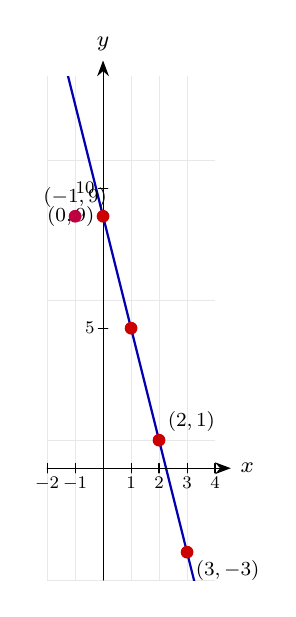
\begin{tikzpicture}[>={Stealth[length=2mm]},font=\footnotesize,line cap=round]
\begin{scope}
\clip (0,0) rectangle (2.133,6.4);
\draw[gray!18] (0,-0.356) grid[xstep=0.356,ystep=1.778] (2.133,6.4);
\draw[blue!70!black,thick] (0,7.467) -- (2.133,-1.067);
\end{scope}
\draw[->] (0,1.422) -- (2.333,1.422) node[right]{$x$};
\draw[->] (0.711,0) -- (0.711,6.6) node[above]{$y$};
\draw (0,1.362) -- (0,1.482) node[below=2pt,scale=0.8]{$-2$};
\draw (0.356,1.362) -- (0.356,1.482) node[below=2pt,scale=0.8]{$-1$};
\draw (1.067,1.362) -- (1.067,1.482) node[below=2pt,scale=0.8]{$1$};
\draw (1.422,1.362) -- (1.422,1.482) node[below=2pt,scale=0.8]{$2$};
\draw (1.778,1.362) -- (1.778,1.482) node[below=2pt,scale=0.8]{$3$};
\draw (2.133,1.362) -- (2.133,1.482) node[below=2pt,scale=0.8]{$4$};
\draw (0.651,3.2) -- (0.771,3.2) node[left=2pt,scale=0.8]{$5$};
\draw (0.651,4.978) -- (0.771,4.978) node[left=2pt,scale=0.8]{$10$};
\fill[red!80!black] (1.067,3.2) circle (2.3pt);
\fill[red!80!black] (1.422,1.778) circle (2.3pt);
\node[above right,scale=0.9] at (1.422,1.778) {$(2,1)$};
\fill[red!80!black] (0.711,4.622) circle (2.3pt);
\node[left,scale=0.9] at (0.711,4.622) {$(0,9)$};
\fill[purple] (0.356,4.622) circle (2.3pt);
\node[above,scale=0.9] at (0.356,4.622) {$(-1,9)$};
\fill[red!80!black] (1.778,0.356) circle (2.3pt);
\node[below right,scale=0.9] at (1.778,0.356) {$(3,-3)$};
\end{tikzpicture}
}
\end{center}
\small The line(s) and key points shown on the coordinate plane.\normalsize

\medskip\hrule

\section*{Equation of a Straight Line 24\quad\small\texttt{(cg1-024)}}
\addcontentsline{toc}{section}{Equation of a Straight Line 24 (cg1-024)}
\textit{Difficulty: Foundation \quad\textbar\quad Marks: 2}

\question{Find the midpoint of the line segment joining \( A(2, 6) \) and \( B(8, 14) \).}

\textbf{Worked solution.}

\textit{Apply the midpoint formula: \( M = \left(\dfrac{x_A + x_B}{2},\ \dfrac{y_A + y_B}{2}\right) \).}
\[\begin{gathered}
M = \left(\dfrac{2 + 8}{2},\ \dfrac{6 + 14}{2}\right) = (5, 10)
\end{gathered}\]
Add the coordinates and halve each.

\begin{answerbox}
\textbf{Final answer:}\quad \(\displaystyle M = (5, 10)\)
\end{answerbox}
\textbf{Diagram.}

\begin{center}
\resizebox{\ifdim\width>\linewidth \linewidth\else \width\fi}{!}{%
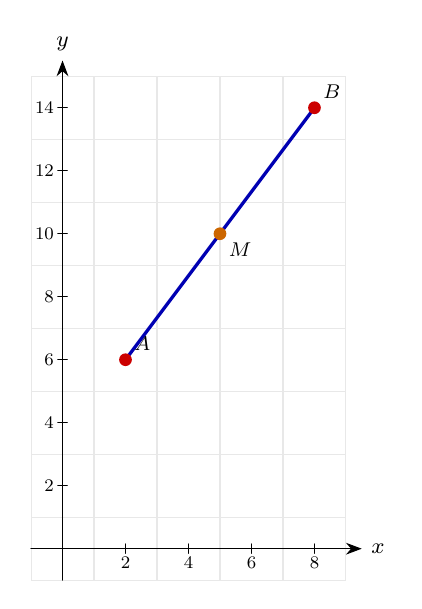
\begin{tikzpicture}[>={Stealth[length=2mm]},font=\footnotesize,line cap=round]
\begin{scope}
\clip (0,0) rectangle (4,6.4);
\draw[gray!18] (-0.4,-0.4) grid[xstep=0.8,ystep=0.8] (4,6.4);
\draw[blue!70!black,very thick] (1.2,2.8) -- (3.6,6);
\end{scope}
\draw[->] (0,0.4) -- (4.2,0.4) node[right]{$x$};
\draw[->] (0.4,0) -- (0.4,6.6) node[above]{$y$};
\draw (1.2,0.34) -- (1.2,0.46) node[below=2pt,scale=0.8]{$2$};
\draw (2,0.34) -- (2,0.46) node[below=2pt,scale=0.8]{$4$};
\draw (2.8,0.34) -- (2.8,0.46) node[below=2pt,scale=0.8]{$6$};
\draw (3.6,0.34) -- (3.6,0.46) node[below=2pt,scale=0.8]{$8$};
\draw (0.34,1.2) -- (0.46,1.2) node[left=2pt,scale=0.8]{$2$};
\draw (0.34,2) -- (0.46,2) node[left=2pt,scale=0.8]{$4$};
\draw (0.34,2.8) -- (0.46,2.8) node[left=2pt,scale=0.8]{$6$};
\draw (0.34,3.6) -- (0.46,3.6) node[left=2pt,scale=0.8]{$8$};
\draw (0.34,4.4) -- (0.46,4.4) node[left=2pt,scale=0.8]{$10$};
\draw (0.34,5.2) -- (0.46,5.2) node[left=2pt,scale=0.8]{$12$};
\draw (0.34,6) -- (0.46,6) node[left=2pt,scale=0.8]{$14$};
\fill[red!80!black] (1.2,2.8) circle (2.3pt);
\node[above right,scale=0.9] at (1.2,2.8) {$A$};
\fill[red!80!black] (3.6,6) circle (2.3pt);
\node[above right,scale=0.9] at (3.6,6) {$B$};
\fill[orange!80!black] (2.4,4.4) circle (2.3pt);
\node[below right,scale=0.9] at (2.4,4.4) {$M$};
\end{tikzpicture}
}
\end{center}
\small The line(s) and key points shown on the coordinate plane.\normalsize

\medskip\hrule

\section*{Equation of a Straight Line 25\quad\small\texttt{(cg1-025)}}
\addcontentsline{toc}{section}{Equation of a Straight Line 25 (cg1-025)}
\textit{Difficulty: Foundation \quad\textbar\quad Marks: 2}

\question{Find the midpoint of the line segment joining \( P(-3, 7) \) and \( Q(5, -1) \).}

\textbf{Worked solution.}

\textit{Apply the midpoint formula.}
\[\begin{gathered}
M = \left(\dfrac{-3 + 5}{2},\ \dfrac{7 + (-1)}{2}\right) = \left(1,\ 3\right)
\end{gathered}\]
Take care with the negative values.

\begin{answerbox}
\textbf{Final answer:}\quad \(\displaystyle M = (1, 3)\)
\end{answerbox}
\textbf{Diagram.}

\begin{center}
\resizebox{\ifdim\width>\linewidth \linewidth\else \width\fi}{!}{%
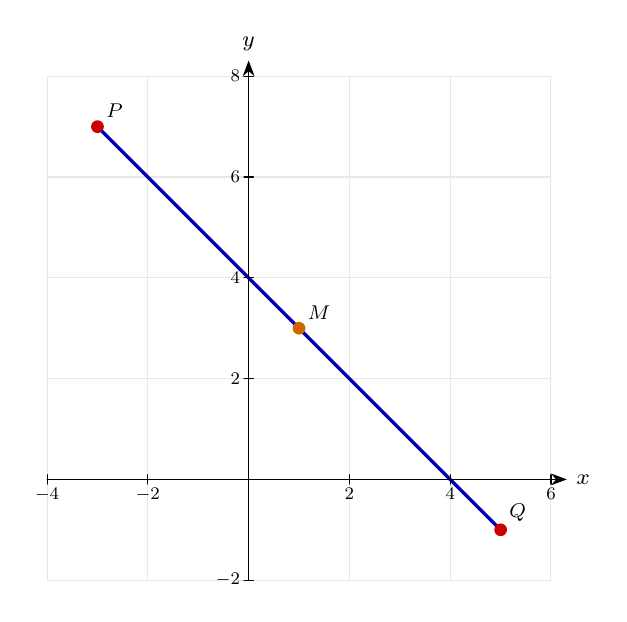
\begin{tikzpicture}[>={Stealth[length=2mm]},font=\footnotesize,line cap=round]
\begin{scope}
\clip (0,0) rectangle (6.4,6.4);
\draw[gray!18] (0,0) grid[xstep=1.28,ystep=1.28] (6.4,6.4);
\draw[blue!70!black,very thick] (0.64,5.76) -- (5.76,0.64);
\end{scope}
\draw[->] (0,1.28) -- (6.6,1.28) node[right]{$x$};
\draw[->] (2.56,0) -- (2.56,6.6) node[above]{$y$};
\draw (0,1.22) -- (0,1.34) node[below=2pt,scale=0.8]{$-4$};
\draw (1.28,1.22) -- (1.28,1.34) node[below=2pt,scale=0.8]{$-2$};
\draw (3.84,1.22) -- (3.84,1.34) node[below=2pt,scale=0.8]{$2$};
\draw (5.12,1.22) -- (5.12,1.34) node[below=2pt,scale=0.8]{$4$};
\draw (6.4,1.22) -- (6.4,1.34) node[below=2pt,scale=0.8]{$6$};
\draw (2.5,0) -- (2.62,0) node[left=2pt,scale=0.8]{$-2$};
\draw (2.5,2.56) -- (2.62,2.56) node[left=2pt,scale=0.8]{$2$};
\draw (2.5,3.84) -- (2.62,3.84) node[left=2pt,scale=0.8]{$4$};
\draw (2.5,5.12) -- (2.62,5.12) node[left=2pt,scale=0.8]{$6$};
\draw (2.5,6.4) -- (2.62,6.4) node[left=2pt,scale=0.8]{$8$};
\fill[red!80!black] (0.64,5.76) circle (2.3pt);
\node[above right,scale=0.9] at (0.64,5.76) {$P$};
\fill[red!80!black] (5.76,0.64) circle (2.3pt);
\node[above right,scale=0.9] at (5.76,0.64) {$Q$};
\fill[orange!80!black] (3.2,3.2) circle (2.3pt);
\node[above right,scale=0.9] at (3.2,3.2) {$M$};
\end{tikzpicture}
}
\end{center}
\small The line(s) and key points shown on the coordinate plane.\normalsize

\medskip\hrule

\section*{Equation of a Straight Line 26\quad\small\texttt{(cg1-026)}}
\addcontentsline{toc}{section}{Equation of a Straight Line 26 (cg1-026)}
\textit{Difficulty: Foundation \quad\textbar\quad Marks: 3}

\question{The midpoint of the line segment \( AB \) is \( M(4, -1) \). If \( A = (1, 3) \), find the coordinates of \( B \).}

\textbf{Worked solution.}

\textit{Step 1: Use the midpoint formula in reverse. If \( M = \left(\frac{x_A + x_B}{2}, \frac{y_A + y_B}{2}\right) \), then:}
\[\begin{gathered}
\dfrac{1 + x_B}{2} = 4 \implies x_B = 7
\end{gathered}\]
Multiply both sides by 2 and solve.

\textit{Step 2: Similarly for the \( y \)-coordinate:}
\[\begin{gathered}
\dfrac{3 + y_B}{2} = -1 \implies y_B = -5
\end{gathered}\]
Multiply both sides by 2 to get \(3 + y_B = -2\), then subtract 3. Watch the sign --- \(-2 - 3 = -5\), not \(-1\).

\begin{answerbox}
\textbf{Final answer:}\quad \(\displaystyle B = (7, -5)\)
\end{answerbox}
\textbf{Diagram.}

\begin{center}
\resizebox{\ifdim\width>\linewidth \linewidth\else \width\fi}{!}{%
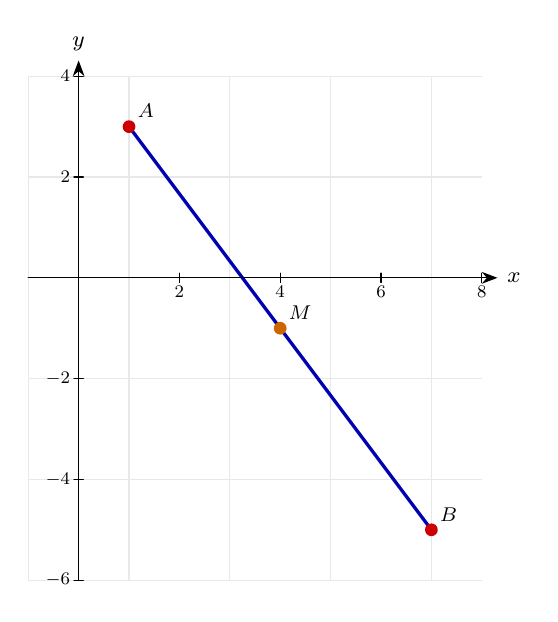
\begin{tikzpicture}[>={Stealth[length=2mm]},font=\footnotesize,line cap=round]
\begin{scope}
\clip (0,0) rectangle (5.76,6.4);
\draw[gray!18] (-0.64,0) grid[xstep=1.28,ystep=1.28] (5.76,6.4);
\draw[blue!70!black,very thick] (1.28,5.76) -- (5.12,0.64);
\end{scope}
\draw[->] (0,3.84) -- (5.96,3.84) node[right]{$x$};
\draw[->] (0.64,0) -- (0.64,6.6) node[above]{$y$};
\draw (1.92,3.78) -- (1.92,3.9) node[below=2pt,scale=0.8]{$2$};
\draw (3.2,3.78) -- (3.2,3.9) node[below=2pt,scale=0.8]{$4$};
\draw (4.48,3.78) -- (4.48,3.9) node[below=2pt,scale=0.8]{$6$};
\draw (5.76,3.78) -- (5.76,3.9) node[below=2pt,scale=0.8]{$8$};
\draw (0.58,0) -- (0.7,0) node[left=2pt,scale=0.8]{$-6$};
\draw (0.58,1.28) -- (0.7,1.28) node[left=2pt,scale=0.8]{$-4$};
\draw (0.58,2.56) -- (0.7,2.56) node[left=2pt,scale=0.8]{$-2$};
\draw (0.58,5.12) -- (0.7,5.12) node[left=2pt,scale=0.8]{$2$};
\draw (0.58,6.4) -- (0.7,6.4) node[left=2pt,scale=0.8]{$4$};
\fill[red!80!black] (1.28,5.76) circle (2.3pt);
\node[above right,scale=0.9] at (1.28,5.76) {$A$};
\fill[orange!80!black] (3.2,3.2) circle (2.3pt);
\node[above right,scale=0.9] at (3.2,3.2) {$M$};
\fill[red!80!black] (5.12,0.64) circle (2.3pt);
\node[above right,scale=0.9] at (5.12,0.64) {$B$};
\end{tikzpicture}
}
\end{center}
\small The line(s) and key points shown on the coordinate plane.\normalsize

\medskip\hrule

\section*{Equation of a Straight Line 27\quad\small\texttt{(cg1-027)}}
\addcontentsline{toc}{section}{Equation of a Straight Line 27 (cg1-027)}
\textit{Difficulty: Foundation \quad\textbar\quad Marks: 5}

\question{Points \( C(a, 5) \) and \( D(6, b) \) lie on the line \( 2x - y + 1 = 0 \). Find the midpoint of \( CD \).}

\textbf{Worked solution.}

\textit{Step 1: Find \( a \): substitute \( y = 5 \) into \( 2x - y + 1 = 0 \).}
\[\begin{gathered}
2a - 5 + 1 = 0 \implies 2a = 4 \implies a = 2
\end{gathered}\]
Since \(C(a, 5)\) lies on the line, its coordinates must satisfy the equation. Replace \(x\) with \(a\), \(y\) with 5, and solve.

\textit{Step 2: Find \( b \): substitute \( x = 6 \) into \( 2x - y + 1 = 0 \).}
\[\begin{gathered}
12 - b + 1 = 0 \implies b = 13
\end{gathered}\]
Same idea for \(D(6, b)\): the point is on the line, so plug in \(x = 6\) and solve for \(b\).

\textit{Step 3: Apply the midpoint formula with \( C = (2, 5) \) and \( D = (6, 13) \).}
\[\begin{gathered}
M = \left(\dfrac{2 + 6}{2},\ \dfrac{5 + 13}{2}\right) = (4, 9)
\end{gathered}\]
Average the \(x\)-coordinates and the \(y\)-coordinates separately to find the midpoint.

\begin{answerbox}
\textbf{Final answer:}\quad \(\displaystyle M = (4, 9)\)
\end{answerbox}
\textbf{Diagram.}

\begin{center}
\resizebox{\ifdim\width>\linewidth \linewidth\else \width\fi}{!}{%
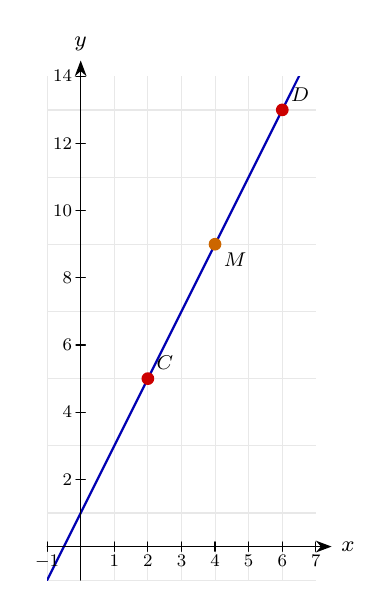
\begin{tikzpicture}[>={Stealth[length=2mm]},font=\footnotesize,line cap=round]
\begin{scope}
\clip (0,0) rectangle (3.413,6.4);
\draw[gray!18] (0,-0.427) grid[xstep=0.427,ystep=0.853] (3.413,6.4);
\draw[blue!70!black,thick] (0,0) -- (3.413,6.827);
\end{scope}
\draw[->] (0,0.427) -- (3.613,0.427) node[right]{$x$};
\draw[->] (0.427,0) -- (0.427,6.6) node[above]{$y$};
\draw (0,0.367) -- (0,0.487) node[below=2pt,scale=0.8]{$-1$};
\draw (0.853,0.367) -- (0.853,0.487) node[below=2pt,scale=0.8]{$1$};
\draw (1.28,0.367) -- (1.28,0.487) node[below=2pt,scale=0.8]{$2$};
\draw (1.707,0.367) -- (1.707,0.487) node[below=2pt,scale=0.8]{$3$};
\draw (2.133,0.367) -- (2.133,0.487) node[below=2pt,scale=0.8]{$4$};
\draw (2.56,0.367) -- (2.56,0.487) node[below=2pt,scale=0.8]{$5$};
\draw (2.987,0.367) -- (2.987,0.487) node[below=2pt,scale=0.8]{$6$};
\draw (3.413,0.367) -- (3.413,0.487) node[below=2pt,scale=0.8]{$7$};
\draw (0.367,1.28) -- (0.487,1.28) node[left=2pt,scale=0.8]{$2$};
\draw (0.367,2.133) -- (0.487,2.133) node[left=2pt,scale=0.8]{$4$};
\draw (0.367,2.987) -- (0.487,2.987) node[left=2pt,scale=0.8]{$6$};
\draw (0.367,3.84) -- (0.487,3.84) node[left=2pt,scale=0.8]{$8$};
\draw (0.367,4.693) -- (0.487,4.693) node[left=2pt,scale=0.8]{$10$};
\draw (0.367,5.547) -- (0.487,5.547) node[left=2pt,scale=0.8]{$12$};
\draw (0.367,6.4) -- (0.487,6.4) node[left=2pt,scale=0.8]{$14$};
\fill[red!80!black] (1.28,2.56) circle (2.3pt);
\node[above right,scale=0.9] at (1.28,2.56) {$C$};
\fill[red!80!black] (2.987,5.973) circle (2.3pt);
\node[above right,scale=0.9] at (2.987,5.973) {$D$};
\fill[orange!80!black] (2.133,4.267) circle (2.3pt);
\node[below right,scale=0.9] at (2.133,4.267) {$M$};
\end{tikzpicture}
}
\end{center}
\small The line(s) and key points shown on the coordinate plane.\normalsize

\medskip\hrule

\section*{Equation of a Straight Line 28\quad\small\texttt{(cg1-028)}}
\addcontentsline{toc}{section}{Equation of a Straight Line 28 (cg1-028)}
\textit{Difficulty: Foundation \quad\textbar\quad Marks: 5}

\question{A taxi charges a fixed fee of \pounds 2 plus \pounds 1.50 per kilometre travelled. \\[3pt] (a) Write an equation in the form \( C = mk + c \), where \( C \) is the total cost in pounds and \( k \) is the distance in kilometres. \\[3pt] (b) Find the cost of a 12 km journey. \\[3pt] (c) A journey costs \pounds 14. How far did the taxi travel?}

\textbf{Worked solution.}

\textit{Step 1: (a) The fixed fee is \( c = 2 \) and the rate per km is \( m = 1.5 \).}
\[\begin{gathered}
C = 1.5k + 2
\end{gathered}\]
The fixed fee is the value of \(C\) when \(k = 0\), so it plays the role of the \(y\)-intercept; the rate per km is the gradient.

\textit{Step 2: (b) Substitute \( k = 12 \).}
\[\begin{gathered}
C = 1.5(12) + 2 = 18 + 2 = 20
\end{gathered}\]
The journey costs \pounds 20.

\textit{Step 3: (c) Set \( C = 14 \) and solve for \( k \).}
\[\begin{gathered}
14 = 1.5k + 2 \implies 1.5k = 12 \implies k = 8
\end{gathered}\]
The taxi travelled 8 km.

\begin{answerbox}
\textbf{Final answer:}\quad (a) \(\displaystyle C = 1.5k + 2\); (b) \pounds 20; (c) 8 km
\end{answerbox}
\textbf{Diagram.}

\begin{center}
\resizebox{\ifdim\width>\linewidth \linewidth\else \width\fi}{!}{%
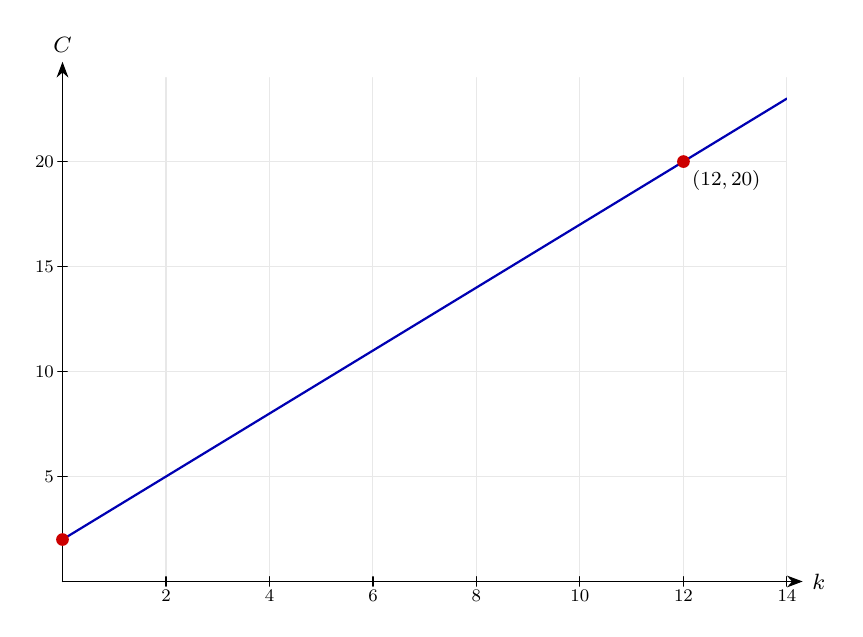
\begin{tikzpicture}[>={Stealth[length=2mm]},font=\footnotesize,line cap=round]
\begin{scope}
\clip (0,0) rectangle (9.2,6.4);
\draw[gray!18] (0,0) grid[xstep=1.314,ystep=1.333] (9.2,6.4);
\draw[blue!70!black,thick] (0,0.533) -- (9.2,6.133);
\end{scope}
\draw[->] (0,0) -- (9.4,0) node[right]{$k$};
\draw[->] (0,0) -- (0,6.6) node[above]{$C$};
\draw (1.314,-0.06) -- (1.314,0.06) node[below=2pt,scale=0.8]{$2$};
\draw (2.629,-0.06) -- (2.629,0.06) node[below=2pt,scale=0.8]{$4$};
\draw (3.943,-0.06) -- (3.943,0.06) node[below=2pt,scale=0.8]{$6$};
\draw (5.257,-0.06) -- (5.257,0.06) node[below=2pt,scale=0.8]{$8$};
\draw (6.571,-0.06) -- (6.571,0.06) node[below=2pt,scale=0.8]{$10$};
\draw (7.886,-0.06) -- (7.886,0.06) node[below=2pt,scale=0.8]{$12$};
\draw (9.2,-0.06) -- (9.2,0.06) node[below=2pt,scale=0.8]{$14$};
\draw (-0.06,1.333) -- (0.06,1.333) node[left=2pt,scale=0.8]{$5$};
\draw (-0.06,2.667) -- (0.06,2.667) node[left=2pt,scale=0.8]{$10$};
\draw (-0.06,4) -- (0.06,4) node[left=2pt,scale=0.8]{$15$};
\draw (-0.06,5.333) -- (0.06,5.333) node[left=2pt,scale=0.8]{$20$};
\fill[red!80!black] (0,0.533) circle (2.3pt);
\fill[red!80!black] (7.886,5.333) circle (2.3pt);
\node[below right,scale=0.9] at (7.886,5.333) {$(12,20)$};
\end{tikzpicture}
}
\end{center}
\small The line(s) and key points shown on the coordinate plane.\normalsize

\medskip\hrule

\section*{Equation of a Straight Line 29\quad\small\texttt{(cg1-029)}}
\addcontentsline{toc}{section}{Equation of a Straight Line 29 (cg1-029)}
\textit{Difficulty: Foundation \quad\textbar\quad Marks: 6}

\question{A candle is 20 cm tall when lit. It burns at a constant rate and is 12 cm tall after 4 hours. \\[3pt] (a) Write an equation for the height \( h \) (in cm) after \( t \) hours. \\[3pt] (b) How tall is the candle after 6 hours? \\[3pt] (c) After how many hours does the candle burn out (reach height 0)?}

\textbf{Worked solution.}

\textit{Step 1: Find the rate of burning (gradient): the candle loses \( 20 - 12 = 8 \) cm in 4 hours.}
\[\begin{gathered}
m = -\dfrac{8}{4} = -2 \text{ cm/hour}
\end{gathered}\]
Negative because height decreases over time.

\textit{Step 2: (a) The initial height is 20 cm, so \( c = 20 \).}
\[\begin{gathered}
h = -2t + 20
\end{gathered}\]
At \(t = 0\) the candle is 20 cm tall, so 20 is the \(h\)-intercept. Combined with the gradient \(-2\), this gives the linear model.

\textit{Step 3: (b) Substitute \( t = 6 \).}
\[\begin{gathered}
h = -2(6) + 20 = 8 \text{ cm}
\end{gathered}\]
Plug the time into the model to find the height after 6 hours.

\textit{Step 4: (c) Set \( h = 0 \).}
\[\begin{gathered}
0 = -2t + 20 \implies t = 10 \text{ hours}
\end{gathered}\]
The candle burns out after 10 hours.

\begin{answerbox}
\textbf{Final answer:}\quad (a) \(\displaystyle h = -2t + 20\); (b) 8 cm; (c) after 10 hours
\end{answerbox}
\textbf{Diagram.}

\begin{center}
\resizebox{\ifdim\width>\linewidth \linewidth\else \width\fi}{!}{%
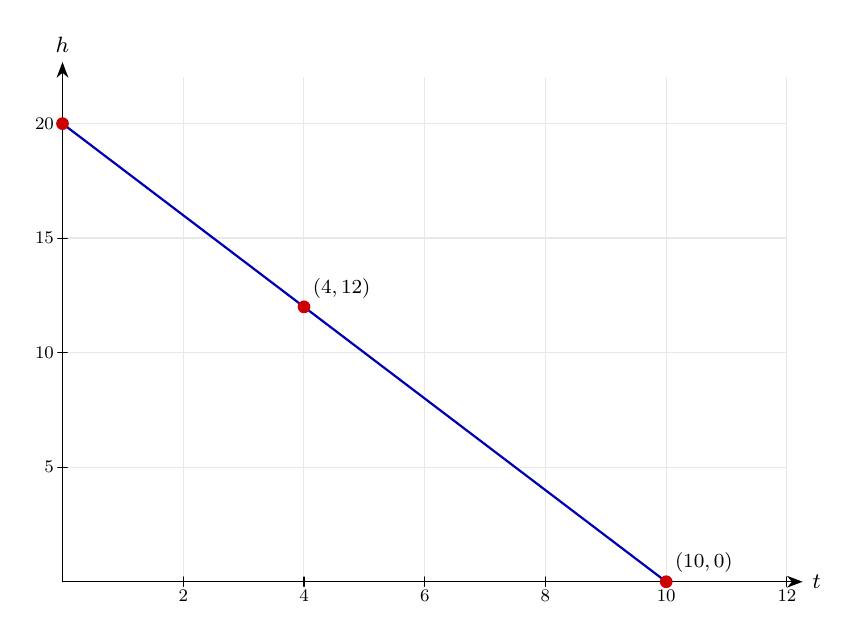
\begin{tikzpicture}[>={Stealth[length=2mm]},font=\footnotesize,line cap=round]
\begin{scope}
\clip (0,0) rectangle (9.2,6.4);
\draw[gray!18] (0,0) grid[xstep=1.533,ystep=1.455] (9.2,6.4);
\draw[blue!70!black,thick] (0,5.818) -- (9.2,-1.164);
\end{scope}
\draw[->] (0,0) -- (9.4,0) node[right]{$t$};
\draw[->] (0,0) -- (0,6.6) node[above]{$h$};
\draw (1.533,-0.06) -- (1.533,0.06) node[below=2pt,scale=0.8]{$2$};
\draw (3.067,-0.06) -- (3.067,0.06) node[below=2pt,scale=0.8]{$4$};
\draw (4.6,-0.06) -- (4.6,0.06) node[below=2pt,scale=0.8]{$6$};
\draw (6.133,-0.06) -- (6.133,0.06) node[below=2pt,scale=0.8]{$8$};
\draw (7.667,-0.06) -- (7.667,0.06) node[below=2pt,scale=0.8]{$10$};
\draw (9.2,-0.06) -- (9.2,0.06) node[below=2pt,scale=0.8]{$12$};
\draw (-0.06,1.455) -- (0.06,1.455) node[left=2pt,scale=0.8]{$5$};
\draw (-0.06,2.909) -- (0.06,2.909) node[left=2pt,scale=0.8]{$10$};
\draw (-0.06,4.364) -- (0.06,4.364) node[left=2pt,scale=0.8]{$15$};
\draw (-0.06,5.818) -- (0.06,5.818) node[left=2pt,scale=0.8]{$20$};
\fill[red!80!black] (0,5.818) circle (2.3pt);
\fill[red!80!black] (3.067,3.491) circle (2.3pt);
\node[above right,scale=0.9] at (3.067,3.491) {$(4,12)$};
\fill[red!80!black] (7.667,0) circle (2.3pt);
\node[above right,scale=0.9] at (7.667,0) {$(10,0)$};
\end{tikzpicture}
}
\end{center}
\small The line(s) and key points shown on the coordinate plane.\normalsize

\medskip\hrule

\section*{Equation of a Straight Line 30\quad\small\texttt{(cg1-030)}}
\addcontentsline{toc}{section}{Equation of a Straight Line 30 (cg1-030)}
\textit{Difficulty: Foundation \quad\textbar\quad Marks: 6}

\question{Two phone contracts are available: \\[3pt] - Contract A: \pounds 10 per month plus 5p per minute of calls. - Contract B: \pounds 25 per month with unlimited calls. \\[3pt] (a) Write equations for the monthly cost \( C_A \) and \( C_B \) in terms of minutes used \( m \). \\[3pt] (b) Find the number of minutes at which both contracts cost the same. \\[3pt] (c) Which contract is cheaper if you use 400 minutes per month?}

\textbf{Worked solution.}

\textit{Step 1: (a) Write the two equations (costs in pounds).}
\[\begin{gathered}
C_A = 0.05m + 10, \quad C_B = 25
\end{gathered}\]
5p = \pounds 0.05 per minute.

\textit{Step 2: (b) Set \( C_A = C_B \) and solve.}
\[\begin{gathered}
0.05m + 10 = 25 \implies 0.05m = 15 \implies m = 300
\end{gathered}\]
Both contracts cost the same at 300 minutes.

\textit{Step 3: (c) At 400 minutes, compare costs.}
\[\begin{gathered}
C_A = 0.05(400) + 10 = 30; \quad C_B = 25
\end{gathered}\]
Contract B is cheaper above 300 minutes.

\begin{answerbox}
\textbf{Final answer:}\quad (a) \(\displaystyle C_A = 0.05m + 10\), \(\displaystyle C_B = 25\); (b) 300 minutes; (c) Contract B
\end{answerbox}
\textbf{Diagram.}

\begin{center}
\resizebox{\ifdim\width>\linewidth \linewidth\else \width\fi}{!}{%
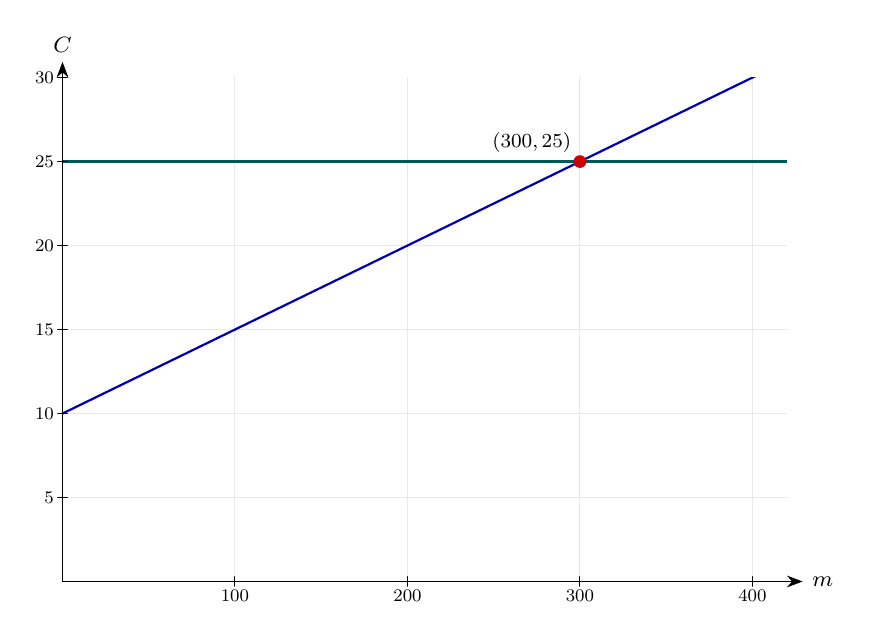
\begin{tikzpicture}[>={Stealth[length=2mm]},font=\footnotesize,line cap=round]
\begin{scope}
\clip (0,0) rectangle (9.2,6.4);
\draw[gray!18] (0,0) grid[xstep=2.19,ystep=1.067] (9.2,6.4);
\draw[blue!70!black,thick] (0,2.133) -- (9.2,6.613);
\draw[teal!70!black,thick] (0,5.333) -- (9.2,5.333);
\end{scope}
\draw[->] (0,0) -- (9.4,0) node[right]{$m$};
\draw[->] (0,0) -- (0,6.6) node[above]{$C$};
\draw (2.19,-0.06) -- (2.19,0.06) node[below=2pt,scale=0.8]{$100$};
\draw (4.381,-0.06) -- (4.381,0.06) node[below=2pt,scale=0.8]{$200$};
\draw (6.571,-0.06) -- (6.571,0.06) node[below=2pt,scale=0.8]{$300$};
\draw (8.762,-0.06) -- (8.762,0.06) node[below=2pt,scale=0.8]{$400$};
\draw (-0.06,1.067) -- (0.06,1.067) node[left=2pt,scale=0.8]{$5$};
\draw (-0.06,2.133) -- (0.06,2.133) node[left=2pt,scale=0.8]{$10$};
\draw (-0.06,3.2) -- (0.06,3.2) node[left=2pt,scale=0.8]{$15$};
\draw (-0.06,4.267) -- (0.06,4.267) node[left=2pt,scale=0.8]{$20$};
\draw (-0.06,5.333) -- (0.06,5.333) node[left=2pt,scale=0.8]{$25$};
\draw (-0.06,6.4) -- (0.06,6.4) node[left=2pt,scale=0.8]{$30$};
\fill[red!80!black] (6.571,5.333) circle (2.3pt);
\node[above left,scale=0.9] at (6.571,5.333) {$(300,25)$};
\end{tikzpicture}
}
\end{center}
\small The line(s) and key points shown on the coordinate plane.\normalsize

\medskip\hrule

\section*{Equation of a Straight Line 31\quad\small\texttt{(cg1-031)}}
\addcontentsline{toc}{section}{Equation of a Straight Line 31 (cg1-031)}
\textit{Difficulty: Foundation \quad\textbar\quad Marks: 3}

\question{Find the equation of the line that is parallel to \( y = 3x - 5 \) and passes through the point \( (2, 7) \). Give your answer in the form \( y = mx + c \).}

\textbf{Worked solution.}

\textit{Step 1: Parallel lines have the same gradient. Here \( m = 3 \).}
\[\begin{gathered}
y = 3x + c
\end{gathered}\]
Two non-vertical lines are parallel iff they share the same gradient. Reading \(m = 3\) off \(y = 3x - 5\) fixes the gradient of our line.

\textit{Step 2: Substitute \( (2, 7) \) to find \( c \).}
\[\begin{gathered}
7 = 3(2) + c \implies c = 1
\end{gathered}\]
The point lies on the line so its coordinates must satisfy the equation. Solve for the unknown intercept.

\textit{Step 3: Write the equation.}
\[\begin{gathered}
y = 3x + 1
\end{gathered}\]
Combine \(m = 3\) and \(c = 1\) into \(y = mx + c\).

\begin{answerbox}
\textbf{Final answer:}\quad \(\displaystyle y = 3x + 1\)
\end{answerbox}
\textbf{Diagram.}

\begin{center}
\resizebox{\ifdim\width>\linewidth \linewidth\else \width\fi}{!}{%
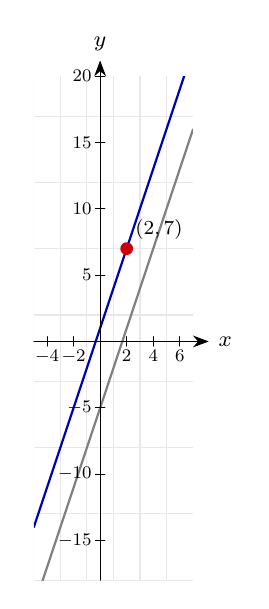
\begin{tikzpicture}[>={Stealth[length=2mm]},font=\footnotesize,line cap=round]
\begin{scope}
\clip (0,0) rectangle (2.021,6.4);
\draw[gray!18] (-0.168,-0.337) grid[xstep=0.337,ystep=0.842] (2.021,6.4);
\draw[gray,thick] (0,-0.337) -- (2.021,5.726);
\draw[blue!70!black,thick] (0,0.674) -- (2.021,6.737);
\end{scope}
\draw[->] (0,3.032) -- (2.221,3.032) node[right]{$x$};
\draw[->] (0.842,0) -- (0.842,6.6) node[above]{$y$};
\draw (0.168,2.972) -- (0.168,3.092) node[below=2pt,scale=0.8]{$-4$};
\draw (0.505,2.972) -- (0.505,3.092) node[below=2pt,scale=0.8]{$-2$};
\draw (1.179,2.972) -- (1.179,3.092) node[below=2pt,scale=0.8]{$2$};
\draw (1.516,2.972) -- (1.516,3.092) node[below=2pt,scale=0.8]{$4$};
\draw (1.853,2.972) -- (1.853,3.092) node[below=2pt,scale=0.8]{$6$};
\draw (0.782,0.505) -- (0.902,0.505) node[left=2pt,scale=0.8]{$-15$};
\draw (0.782,1.347) -- (0.902,1.347) node[left=2pt,scale=0.8]{$-10$};
\draw (0.782,2.189) -- (0.902,2.189) node[left=2pt,scale=0.8]{$-5$};
\draw (0.782,3.874) -- (0.902,3.874) node[left=2pt,scale=0.8]{$5$};
\draw (0.782,4.716) -- (0.902,4.716) node[left=2pt,scale=0.8]{$10$};
\draw (0.782,5.558) -- (0.902,5.558) node[left=2pt,scale=0.8]{$15$};
\draw (0.782,6.4) -- (0.902,6.4) node[left=2pt,scale=0.8]{$20$};
\fill[red!80!black] (1.179,4.211) circle (2.3pt);
\node[above right,scale=0.9] at (1.179,4.211) {$(2,7)$};
\end{tikzpicture}
}
\end{center}
\small The line(s) and key points shown on the coordinate plane.\normalsize

\medskip\hrule

\section*{Equation of a Straight Line 32\quad\small\texttt{(cg1-032)}}
\addcontentsline{toc}{section}{Equation of a Straight Line 32 (cg1-032)}
\textit{Difficulty: Foundation \quad\textbar\quad Marks: 4}

\question{Find the equation of the line perpendicular to \( y = 2x + 1 \) that passes through the point \( (4, 3) \). Give your answer in the form \( y = mx + c \).}

\textbf{Worked solution.}

\textit{Step 1: The gradient of the original line is \( 2 \). Perpendicular lines satisfy \( m_1 \times m_2 = -1 \).}
\[\begin{gathered}
m_2 = -\dfrac{1}{2}
\end{gathered}\]
The perpendicular gradient is the negative reciprocal.

\textit{Step 2: Use \( y = -\frac{1}{2}x + c \) and substitute \( (4, 3) \).}
\[\begin{gathered}
3 = -\dfrac{1}{2}(4) + c \implies 3 = -2 + c \implies c = 5
\end{gathered}\]
Substituting the given point pins down the intercept. Adding 2 to both sides gives \(c = 5\).

\textit{Step 3: Write the equation.}
\[\begin{gathered}
y = -\dfrac{1}{2}x + 5
\end{gathered}\]
Combine \(m = -\tfrac{1}{2}\) and \(c = 5\) into \(y = mx + c\).

\begin{answerbox}
\textbf{Final answer:}\quad \(\displaystyle y = -\dfrac{1}{2}x + 5\)
\end{answerbox}
\textbf{Diagram.}

\begin{center}
\resizebox{\ifdim\width>\linewidth \linewidth\else \width\fi}{!}{%
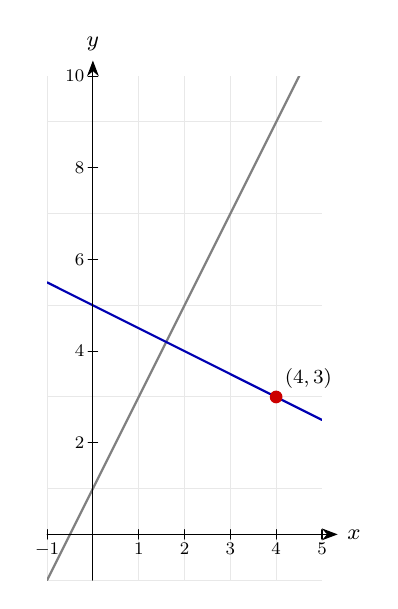
\begin{tikzpicture}[>={Stealth[length=2mm]},font=\footnotesize,line cap=round]
\begin{scope}
\clip (0,0) rectangle (3.491,6.4);
\draw[gray!18] (0,-0.582) grid[xstep=0.582,ystep=1.164] (3.491,6.4);
\draw[gray,thick] (0,0) -- (3.491,6.982);
\draw[blue!70!black,thick] (0,3.782) -- (3.491,2.036);
\end{scope}
\draw[->] (0,0.582) -- (3.691,0.582) node[right]{$x$};
\draw[->] (0.582,0) -- (0.582,6.6) node[above]{$y$};
\draw (0,0.522) -- (0,0.642) node[below=2pt,scale=0.8]{$-1$};
\draw (1.164,0.522) -- (1.164,0.642) node[below=2pt,scale=0.8]{$1$};
\draw (1.745,0.522) -- (1.745,0.642) node[below=2pt,scale=0.8]{$2$};
\draw (2.327,0.522) -- (2.327,0.642) node[below=2pt,scale=0.8]{$3$};
\draw (2.909,0.522) -- (2.909,0.642) node[below=2pt,scale=0.8]{$4$};
\draw (3.491,0.522) -- (3.491,0.642) node[below=2pt,scale=0.8]{$5$};
\draw (0.522,1.745) -- (0.642,1.745) node[left=2pt,scale=0.8]{$2$};
\draw (0.522,2.909) -- (0.642,2.909) node[left=2pt,scale=0.8]{$4$};
\draw (0.522,4.073) -- (0.642,4.073) node[left=2pt,scale=0.8]{$6$};
\draw (0.522,5.236) -- (0.642,5.236) node[left=2pt,scale=0.8]{$8$};
\draw (0.522,6.4) -- (0.642,6.4) node[left=2pt,scale=0.8]{$10$};
\fill[red!80!black] (2.909,2.327) circle (2.3pt);
\node[above right,scale=0.9] at (2.909,2.327) {$(4,3)$};
\end{tikzpicture}
}
\end{center}
\small The line(s) and key points shown on the coordinate plane.\normalsize

\medskip\hrule

\section*{Equation of a Straight Line 33\quad\small\texttt{(cg1-033)}}
\addcontentsline{toc}{section}{Equation of a Straight Line 33 (cg1-033)}
\textit{Difficulty: Foundation \quad\textbar\quad Marks: 5}

\question{Line \( L_1 \) passes through \( (0, 4) \) and \( (3, 10) \). Line \( L_2 \) is perpendicular to \( L_1 \) and passes through \( (6, 1) \). Find the equation of \( L_2 \) in the form \( y = mx + c \).}

\textbf{Worked solution.}

\textit{Step 1: Find the gradient of \( L_1 \).}
\[\begin{gathered}
m_1 = \dfrac{10 - 4}{3 - 0} = \dfrac{6}{3} = 2
\end{gathered}\]
Apply \(m = \frac{y_2 - y_1}{x_2 - x_1}\) to the two given points on \(L_1\).

\textit{Step 2: The gradient of \( L_2 \) is the negative reciprocal.}
\[\begin{gathered}
m_2 = -\dfrac{1}{2}
\end{gathered}\]
Perpendicular gradients satisfy \(m_1 m_2 = -1\), so \(m_2 = -\tfrac{1}{m_1}\). Flip and negate.

\textit{Step 3: Use \( y = -\frac{1}{2}x + c \) and substitute \( (6, 1) \).}
\[\begin{gathered}
1 = -\dfrac{1}{2}(6) + c \implies 1 = -3 + c \implies c = 4
\end{gathered}\]
The point lies on \(L_2\), so its coordinates satisfy the equation. Solve for the intercept.

\textit{Step 4: Write the equation.}
\[\begin{gathered}
y = -\dfrac{1}{2}x + 4
\end{gathered}\]
Combine \(m_2 = -\tfrac{1}{2}\) and \(c = 4\) into \(y = mx + c\).

\begin{answerbox}
\textbf{Final answer:}\quad \(\displaystyle y = -\dfrac{1}{2}x + 4\)
\end{answerbox}
\textbf{Diagram.}

\begin{center}
\resizebox{\ifdim\width>\linewidth \linewidth\else \width\fi}{!}{%
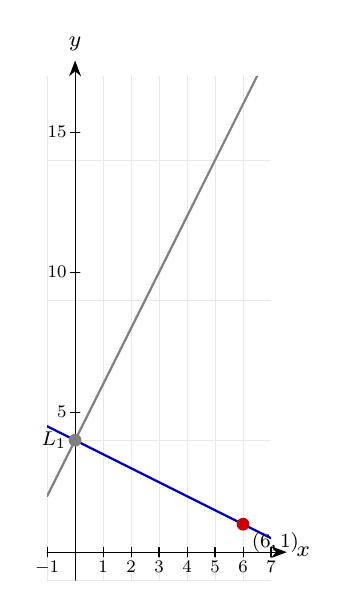
\begin{tikzpicture}[>={Stealth[length=2mm]},font=\footnotesize,line cap=round]
\begin{scope}
\clip (0,0) rectangle (2.844,6.4);
\draw[gray!18] (0,-1.422) grid[xstep=0.356,ystep=1.778] (2.844,6.4);
\draw[gray,thick] (0,1.067) -- (2.844,6.756);
\draw[blue!70!black,thick] (0,1.956) -- (2.844,0.533);
\end{scope}
\draw[->] (0,0.356) -- (3.044,0.356) node[right]{$x$};
\draw[->] (0.356,0) -- (0.356,6.6) node[above]{$y$};
\draw (0,0.296) -- (0,0.416) node[below=2pt,scale=0.8]{$-1$};
\draw (0.711,0.296) -- (0.711,0.416) node[below=2pt,scale=0.8]{$1$};
\draw (1.067,0.296) -- (1.067,0.416) node[below=2pt,scale=0.8]{$2$};
\draw (1.422,0.296) -- (1.422,0.416) node[below=2pt,scale=0.8]{$3$};
\draw (1.778,0.296) -- (1.778,0.416) node[below=2pt,scale=0.8]{$4$};
\draw (2.133,0.296) -- (2.133,0.416) node[below=2pt,scale=0.8]{$5$};
\draw (2.489,0.296) -- (2.489,0.416) node[below=2pt,scale=0.8]{$6$};
\draw (2.844,0.296) -- (2.844,0.416) node[below=2pt,scale=0.8]{$7$};
\draw (0.296,2.133) -- (0.416,2.133) node[left=2pt,scale=0.8]{$5$};
\draw (0.296,3.911) -- (0.416,3.911) node[left=2pt,scale=0.8]{$10$};
\draw (0.296,5.689) -- (0.416,5.689) node[left=2pt,scale=0.8]{$15$};
\fill[gray] (0.356,1.778) circle (2.3pt);
\node[left,scale=0.9] at (0.356,1.778) {$L_1$};
\fill[red!80!black] (2.489,0.711) circle (2.3pt);
\node[below right,scale=0.9] at (2.489,0.711) {$(6,1)$};
\end{tikzpicture}
}
\end{center}
\small The line(s) and key points shown on the coordinate plane.\normalsize

\medskip\hrule

\section*{Equation of a Straight Line 34\quad\small\texttt{(cg1-034)}}
\addcontentsline{toc}{section}{Equation of a Straight Line 34 (cg1-034)}
\textit{Difficulty: Foundation \quad\textbar\quad Marks: 8}

\question{The line \( L \) passes through the points \( A(1, 5) \) and \( B(7, 2) \). \\[3pt] (a) Find the gradient of \( L \). \\[3pt] (b) Find the equation of \( L \) in the form \( ax + by + c = 0 \), where \( a \), \( b \) and \( c \) are integers. \\[3pt] (c) The point \( C \) lies on \( L \) and has \( x \)-coordinate 13. Find the \( y \)-coordinate of \( C \). \\[3pt] (d) Find the midpoint of \( AB \).}

\textbf{Worked solution.}

\textit{Step 1: (a) Find the gradient.}
\[\begin{gathered}
m = \dfrac{2 - 5}{7 - 1} = \dfrac{-3}{6} = -\dfrac{1}{2}
\end{gathered}\]
Apply \(m = \frac{y_2 - y_1}{x_2 - x_1}\). The negative result means \(L\) slopes downward left to right.

\textit{Step 2: (b) Find the equation. Use \( y = -\frac{1}{2}x + c \) with \( (1, 5) \).}
\[\begin{gathered}
5 = -\tfrac{1}{2}(1) + c \implies c = \tfrac{11}{2}
\end{gathered}\]
Substitute the point into \(y = mx + c\) and solve. Adding \(\tfrac{1}{2}\) to 5 gives \(\tfrac{11}{2}\).

\textit{Step 3: Multiply through by 2 and rearrange into \( ax + by + c = 0 \).}
\[\begin{gathered}
2y = -x + 11 \quad\quad \Rightarrow \quad\quad x + 2y - 11 = 0
\end{gathered}\]
Multiplying by 2 clears the fraction so that \(a, b, c\) come out as integers, as required.

\textit{Step 4: (c) Substitute \( x = 13 \) into \( x + 2y - 11 = 0 \).}
\[\begin{gathered}
13 + 2y - 11 = 0 \implies 2y = -2 \implies y = -1
\end{gathered}\]
Since \(C\) lies on \(L\), its coordinates must satisfy the line equation. Solve for the missing \(y\).

\textit{Step 5: (d) Apply the midpoint formula.}
\[\begin{gathered}
M = \left(\dfrac{1+7}{2},\ \dfrac{5+2}{2}\right) = \left(4,\ 3.5\right)
\end{gathered}\]
Average the \(x\)-coordinates and the \(y\)-coordinates separately.

\begin{answerbox}
\textbf{Final answer:}\quad (a) \(\displaystyle -\dfrac{1}{2}\); (b) \(\displaystyle x + 2y - 11 = 0\); (c) \(\displaystyle y = -1\); (d) \(\displaystyle M = (4,\ 3.5)\)
\end{answerbox}
\textbf{Diagram.}

\begin{center}
\resizebox{\ifdim\width>\linewidth \linewidth\else \width\fi}{!}{%
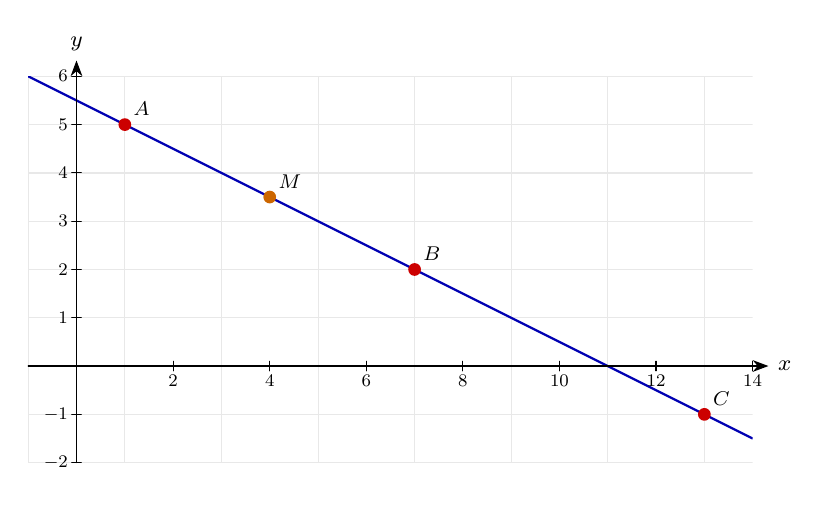
\begin{tikzpicture}[>={Stealth[length=2mm]},font=\footnotesize,line cap=round]
\begin{scope}
\clip (0,0) rectangle (9.2,4.907);
\draw[gray!18] (-0.613,0) grid[xstep=1.227,ystep=0.613] (9.2,4.907);
\draw[blue!70!black,thick] (0,4.907) -- (9.2,0.307);
\end{scope}
\draw[->] (0,1.227) -- (9.4,1.227) node[right]{$x$};
\draw[->] (0.613,0) -- (0.613,5.107) node[above]{$y$};
\draw (1.84,1.167) -- (1.84,1.287) node[below=2pt,scale=0.8]{$2$};
\draw (3.067,1.167) -- (3.067,1.287) node[below=2pt,scale=0.8]{$4$};
\draw (4.293,1.167) -- (4.293,1.287) node[below=2pt,scale=0.8]{$6$};
\draw (5.52,1.167) -- (5.52,1.287) node[below=2pt,scale=0.8]{$8$};
\draw (6.747,1.167) -- (6.747,1.287) node[below=2pt,scale=0.8]{$10$};
\draw (7.973,1.167) -- (7.973,1.287) node[below=2pt,scale=0.8]{$12$};
\draw (9.2,1.167) -- (9.2,1.287) node[below=2pt,scale=0.8]{$14$};
\draw (0.553,0) -- (0.673,0) node[left=2pt,scale=0.8]{$-2$};
\draw (0.553,0.613) -- (0.673,0.613) node[left=2pt,scale=0.8]{$-1$};
\draw (0.553,1.84) -- (0.673,1.84) node[left=2pt,scale=0.8]{$1$};
\draw (0.553,2.453) -- (0.673,2.453) node[left=2pt,scale=0.8]{$2$};
\draw (0.553,3.067) -- (0.673,3.067) node[left=2pt,scale=0.8]{$3$};
\draw (0.553,3.68) -- (0.673,3.68) node[left=2pt,scale=0.8]{$4$};
\draw (0.553,4.293) -- (0.673,4.293) node[left=2pt,scale=0.8]{$5$};
\draw (0.553,4.907) -- (0.673,4.907) node[left=2pt,scale=0.8]{$6$};
\fill[red!80!black] (1.227,4.293) circle (2.3pt);
\node[above right,scale=0.9] at (1.227,4.293) {$A$};
\fill[red!80!black] (4.907,2.453) circle (2.3pt);
\node[above right,scale=0.9] at (4.907,2.453) {$B$};
\fill[red!80!black] (8.587,0.613) circle (2.3pt);
\node[above right,scale=0.9] at (8.587,0.613) {$C$};
\fill[orange!80!black] (3.067,3.373) circle (2.3pt);
\node[above right,scale=0.9] at (3.067,3.373) {$M$};
\end{tikzpicture}
}
\end{center}
\small The line(s) and key points shown on the coordinate plane.\normalsize

\medskip\hrule

\section*{Equation of a Straight Line 35\quad\small\texttt{(cg1-035)}}
\addcontentsline{toc}{section}{Equation of a Straight Line 35 (cg1-035)}
\textit{Difficulty: Foundation \quad\textbar\quad Marks: 9}

\question{The points \( P(2, k) \) and \( Q(6, 1) \) lie on the line \( 3x + 4y - 10 = 0 \). \\[3pt] (a) Find the value of \( k \). \\[3pt] (b) Find the midpoint \( M \) of \( PQ \). \\[3pt] (c) Find the equation of the line through \( M \) that is perpendicular to \( PQ \). Give your answer in the form \( y = mx + c \).}

\textbf{Worked solution.}

\textit{Step 1: (a) Substitute \( P(2, k) \) into \( 3x + 4y - 10 = 0 \).}
\[\begin{gathered}
3(2) + 4k - 10 = 0 \implies 6 + 4k - 10 = 0 \implies 4k = 4 \implies k = 1
\end{gathered}\]
Since \(P\) lies on the line, its coordinates must satisfy the equation. This gives a linear equation in \(k\) which we can solve.

\textit{Step 2: (b) Now \( P = (2, 1) \) and \( Q = (6, 1) \). Find the midpoint.}
\[\begin{gathered}
M = \left(\dfrac{2+6}{2},\ \dfrac{1+1}{2}\right) = (4, 1)
\end{gathered}\]
Both points have the same \( y \)-coordinate, so \( PQ \) is horizontal.

\textit{Step 3: (c) The gradient of \( PQ \): since \( P \) and \( Q \) have the same \( y \)-value, \( m_{PQ} = 0 \). The perpendicular is vertical.}
\[\begin{gathered}
x = 4
\end{gathered}\]
A line perpendicular to a horizontal line is vertical, passing through \( x = 4 \).

\begin{answerbox}
\textbf{Final answer:}\quad (a) \(\displaystyle k = 1\); (b) \(\displaystyle M = (4, 1)\); (c) \(\displaystyle x = 4\) (a vertical line)
\end{answerbox}
\textbf{Diagram.}

\begin{center}
\resizebox{\ifdim\width>\linewidth \linewidth\else \width\fi}{!}{%
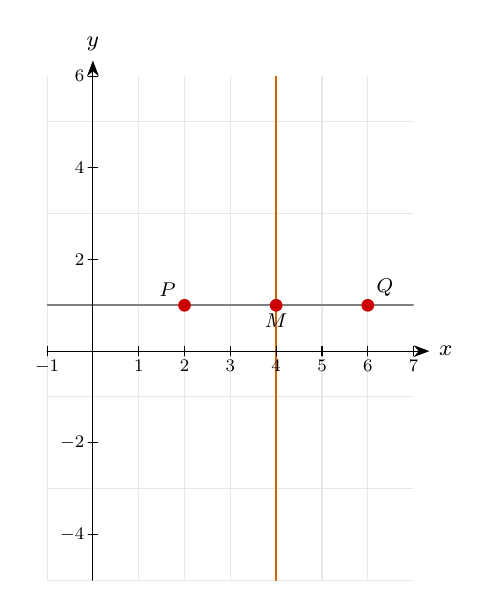
\begin{tikzpicture}[>={Stealth[length=2mm]},font=\footnotesize,line cap=round]
\begin{scope}
\clip (0,0) rectangle (4.655,6.4);
\draw[gray!18] (0,-0.582) grid[xstep=0.582,ystep=1.164] (4.655,6.4);
\draw[gray,thick] (0,3.491) -- (4.655,3.491);
\draw[orange!80!black,thick] (2.909,0) -- (2.909,6.4);
\end{scope}
\draw[->] (0,2.909) -- (4.855,2.909) node[right]{$x$};
\draw[->] (0.582,0) -- (0.582,6.6) node[above]{$y$};
\draw (0,2.849) -- (0,2.969) node[below=2pt,scale=0.8]{$-1$};
\draw (1.164,2.849) -- (1.164,2.969) node[below=2pt,scale=0.8]{$1$};
\draw (1.745,2.849) -- (1.745,2.969) node[below=2pt,scale=0.8]{$2$};
\draw (2.327,2.849) -- (2.327,2.969) node[below=2pt,scale=0.8]{$3$};
\draw (2.909,2.849) -- (2.909,2.969) node[below=2pt,scale=0.8]{$4$};
\draw (3.491,2.849) -- (3.491,2.969) node[below=2pt,scale=0.8]{$5$};
\draw (4.073,2.849) -- (4.073,2.969) node[below=2pt,scale=0.8]{$6$};
\draw (4.655,2.849) -- (4.655,2.969) node[below=2pt,scale=0.8]{$7$};
\draw (0.522,0.582) -- (0.642,0.582) node[left=2pt,scale=0.8]{$-4$};
\draw (0.522,1.745) -- (0.642,1.745) node[left=2pt,scale=0.8]{$-2$};
\draw (0.522,4.073) -- (0.642,4.073) node[left=2pt,scale=0.8]{$2$};
\draw (0.522,5.236) -- (0.642,5.236) node[left=2pt,scale=0.8]{$4$};
\draw (0.522,6.4) -- (0.642,6.4) node[left=2pt,scale=0.8]{$6$};
\fill[red!80!black] (1.745,3.491) circle (2.3pt);
\node[above left,scale=0.9] at (1.745,3.491) {$P$};
\fill[red!80!black] (4.073,3.491) circle (2.3pt);
\node[above right,scale=0.9] at (4.073,3.491) {$Q$};
\fill[red!80!black] (2.909,3.491) circle (2.3pt);
\node[below,scale=0.9] at (2.909,3.491) {$M$};
\end{tikzpicture}
}
\end{center}
\small The line(s) and key points shown on the coordinate plane.\normalsize

\medskip\hrule

\section*{Equation of a Straight Line 36\quad\small\texttt{(cg1-036)}}
\addcontentsline{toc}{section}{Equation of a Straight Line 36 (cg1-036)}
\textit{Difficulty: Foundation \quad\textbar\quad Marks: 2}

\question{Find the equation of the line with gradient \( 3 \) passing through the point \( (1, 5) \). Give your answer in the form \( y = mx + c \).}

\textbf{Worked solution.}

\textit{Step 1: Use y - y1 = m(x - x1)}
\[\begin{gathered}
y - 5 = 3(x - 1) = 3x - 3
\end{gathered}\]
Substitute gradient and point.

\textit{Step 2: Rearrange}
\[\begin{gathered}
y = 3x + 2
\end{gathered}\]
Add 5 to both sides.

\begin{answerbox}
\textbf{Final answer:}\quad \(\displaystyle y = 3x + 2\)
\end{answerbox}
\textbf{Diagram.}

\begin{center}
\resizebox{\ifdim\width>\linewidth \linewidth\else \width\fi}{!}{%
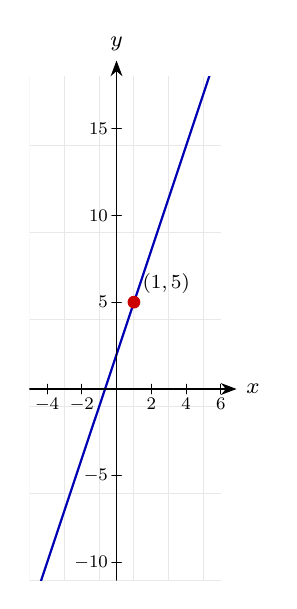
\begin{tikzpicture}[>={Stealth[length=2mm]},font=\footnotesize,line cap=round]
\begin{scope}
\clip (0,0) rectangle (2.428,6.4);
\draw[gray!18] (-0.221,-0.883) grid[xstep=0.441,ystep=1.103] (2.428,6.4);
\draw[blue!70!black,thick] (0,-0.441) -- (2.428,6.841);
\end{scope}
\draw[->] (0,2.428) -- (2.628,2.428) node[right]{$x$};
\draw[->] (1.103,0) -- (1.103,6.6) node[above]{$y$};
\draw (0.221,2.368) -- (0.221,2.488) node[below=2pt,scale=0.8]{$-4$};
\draw (0.662,2.368) -- (0.662,2.488) node[below=2pt,scale=0.8]{$-2$};
\draw (1.545,2.368) -- (1.545,2.488) node[below=2pt,scale=0.8]{$2$};
\draw (1.986,2.368) -- (1.986,2.488) node[below=2pt,scale=0.8]{$4$};
\draw (2.428,2.368) -- (2.428,2.488) node[below=2pt,scale=0.8]{$6$};
\draw (1.043,0.221) -- (1.163,0.221) node[left=2pt,scale=0.8]{$-10$};
\draw (1.043,1.324) -- (1.163,1.324) node[left=2pt,scale=0.8]{$-5$};
\draw (1.043,3.531) -- (1.163,3.531) node[left=2pt,scale=0.8]{$5$};
\draw (1.043,4.634) -- (1.163,4.634) node[left=2pt,scale=0.8]{$10$};
\draw (1.043,5.738) -- (1.163,5.738) node[left=2pt,scale=0.8]{$15$};
\fill[red!80!black] (1.324,3.531) circle (2.3pt);
\node[above right,scale=0.9] at (1.324,3.531) {$(1,5)$};
\end{tikzpicture}
}
\end{center}
\small The line(s) and key points shown on the coordinate plane.\normalsize

\medskip\hrule

\section*{Equation of a Straight Line 37\quad\small\texttt{(cg1-037)}}
\addcontentsline{toc}{section}{Equation of a Straight Line 37 (cg1-037)}
\textit{Difficulty: Foundation \quad\textbar\quad Marks: 3}

\question{Find the equation of the line passing through \( (2, 7) \) and \( (6, 3) \).}

\textbf{Worked solution.}

\textit{Step 1: Find gradient}
\[\begin{gathered}
m = \frac{3 - 7}{6 - 2} = \frac{-4}{4} = -1
\end{gathered}\]
Change in y over change in x.

\textit{Step 2: Use point-slope form}
\[\begin{gathered}
y - 7 = -1(x - 2) \implies y = -x + 9
\end{gathered}\]
Substitute into \(y - y_1 = m(x - x_1)\) using either point.

\begin{answerbox}
\textbf{Final answer:}\quad \(\displaystyle y = -x + 9\)
\end{answerbox}
\textbf{Common mistake.} Using either point gives the same final equation. With \((6,3)\): \(y - 3 = -1(x - 6) \implies y = -x + 9\).

\textbf{Diagram.}

\begin{center}
\resizebox{\ifdim\width>\linewidth \linewidth\else \width\fi}{!}{%
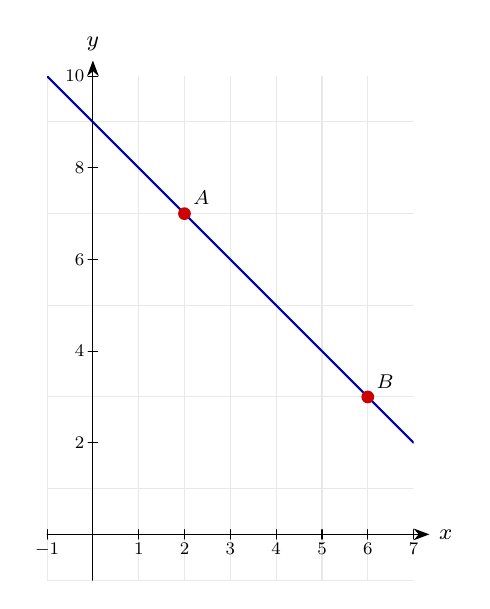
\begin{tikzpicture}[>={Stealth[length=2mm]},font=\footnotesize,line cap=round]
\begin{scope}
\clip (0,0) rectangle (4.655,6.4);
\draw[gray!18] (0,-0.582) grid[xstep=0.582,ystep=1.164] (4.655,6.4);
\draw[blue!70!black,thick] (0,6.4) -- (4.655,1.745);
\end{scope}
\draw[->] (0,0.582) -- (4.855,0.582) node[right]{$x$};
\draw[->] (0.582,0) -- (0.582,6.6) node[above]{$y$};
\draw (0,0.522) -- (0,0.642) node[below=2pt,scale=0.8]{$-1$};
\draw (1.164,0.522) -- (1.164,0.642) node[below=2pt,scale=0.8]{$1$};
\draw (1.745,0.522) -- (1.745,0.642) node[below=2pt,scale=0.8]{$2$};
\draw (2.327,0.522) -- (2.327,0.642) node[below=2pt,scale=0.8]{$3$};
\draw (2.909,0.522) -- (2.909,0.642) node[below=2pt,scale=0.8]{$4$};
\draw (3.491,0.522) -- (3.491,0.642) node[below=2pt,scale=0.8]{$5$};
\draw (4.073,0.522) -- (4.073,0.642) node[below=2pt,scale=0.8]{$6$};
\draw (4.655,0.522) -- (4.655,0.642) node[below=2pt,scale=0.8]{$7$};
\draw (0.522,1.745) -- (0.642,1.745) node[left=2pt,scale=0.8]{$2$};
\draw (0.522,2.909) -- (0.642,2.909) node[left=2pt,scale=0.8]{$4$};
\draw (0.522,4.073) -- (0.642,4.073) node[left=2pt,scale=0.8]{$6$};
\draw (0.522,5.236) -- (0.642,5.236) node[left=2pt,scale=0.8]{$8$};
\draw (0.522,6.4) -- (0.642,6.4) node[left=2pt,scale=0.8]{$10$};
\fill[red!80!black] (1.745,4.655) circle (2.3pt);
\node[above right,scale=0.9] at (1.745,4.655) {$A$};
\fill[red!80!black] (4.073,2.327) circle (2.3pt);
\node[above right,scale=0.9] at (4.073,2.327) {$B$};
\end{tikzpicture}
}
\end{center}
\small The line(s) and key points shown on the coordinate plane.\normalsize

\medskip\hrule

\section*{Equation of a Straight Line 38\quad\small\texttt{(cg1-038)}}
\addcontentsline{toc}{section}{Equation of a Straight Line 38 (cg1-038)}
\textit{Difficulty: Foundation \quad\textbar\quad Marks: 2}

\question{Find the gradient of the line \( 5x + 2y - 8 = 0 \).}

\textbf{Worked solution.}

\textit{Rearrange to y = mx + c}
\[\begin{gathered}
2y = -5x + 8 \implies y = -\frac{5}{2}x + 4
\end{gathered}\]
Isolate y.

\begin{answerbox}
\textbf{Final answer:}\quad \(\displaystyle -\frac{5}{2}\)
\end{answerbox}
\textbf{Diagram.}

\begin{center}
\resizebox{\ifdim\width>\linewidth \linewidth\else \width\fi}{!}{%
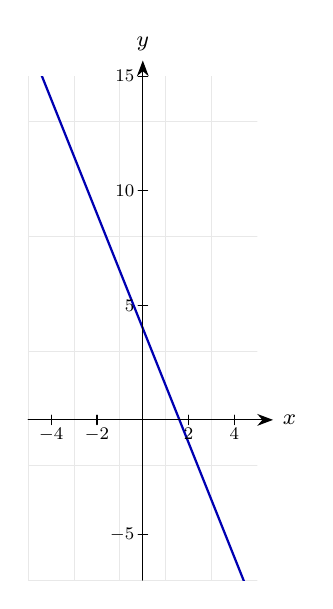
\begin{tikzpicture}[>={Stealth[length=2mm]},font=\footnotesize,line cap=round]
\begin{scope}
\clip (0,0) rectangle (2.909,6.4);
\draw[gray!18] (-0.291,-0.873) grid[xstep=0.582,ystep=1.455] (2.909,6.4);
\draw[blue!70!black,thick] (0,6.836) -- (2.909,-0.436);
\end{scope}
\draw[->] (0,2.036) -- (3.109,2.036) node[right]{$x$};
\draw[->] (1.455,0) -- (1.455,6.6) node[above]{$y$};
\draw (0.291,1.976) -- (0.291,2.096) node[below=2pt,scale=0.8]{$-4$};
\draw (0.873,1.976) -- (0.873,2.096) node[below=2pt,scale=0.8]{$-2$};
\draw (2.036,1.976) -- (2.036,2.096) node[below=2pt,scale=0.8]{$2$};
\draw (2.618,1.976) -- (2.618,2.096) node[below=2pt,scale=0.8]{$4$};
\draw (1.395,0.582) -- (1.515,0.582) node[left=2pt,scale=0.8]{$-5$};
\draw (1.395,3.491) -- (1.515,3.491) node[left=2pt,scale=0.8]{$5$};
\draw (1.395,4.945) -- (1.515,4.945) node[left=2pt,scale=0.8]{$10$};
\draw (1.395,6.4) -- (1.515,6.4) node[left=2pt,scale=0.8]{$15$};
\end{tikzpicture}
}
\end{center}
\small The line(s) and key points shown on the coordinate plane.\normalsize

\medskip\hrule

\section*{Equation of a Straight Line 39\quad\small\texttt{(cg1-039)}}
\addcontentsline{toc}{section}{Equation of a Straight Line 39 (cg1-039)}
\textit{Difficulty: Foundation \quad\textbar\quad Marks: 3}

\question{A line has gradient \( \frac{2}{3} \) and passes through \( (-3, 1) \). Find where it crosses the y-axis.}

\textbf{Worked solution.}

\textit{Step 1: Find equation}
\[\begin{gathered}
y - 1 = \frac{2}{3}(x + 3) = \frac{2}{3}x + 2
\end{gathered}\]
Point-slope form.

\textit{Step 2: Simplify}
\[\begin{gathered}
y = \frac{2}{3}x + 3
\end{gathered}\]
y-intercept is (0, 3).

\begin{answerbox}
\textbf{Final answer:}\quad \(\displaystyle (0, 3)\)
\end{answerbox}
\textbf{Diagram.}

\begin{center}
\resizebox{\ifdim\width>\linewidth \linewidth\else \width\fi}{!}{%
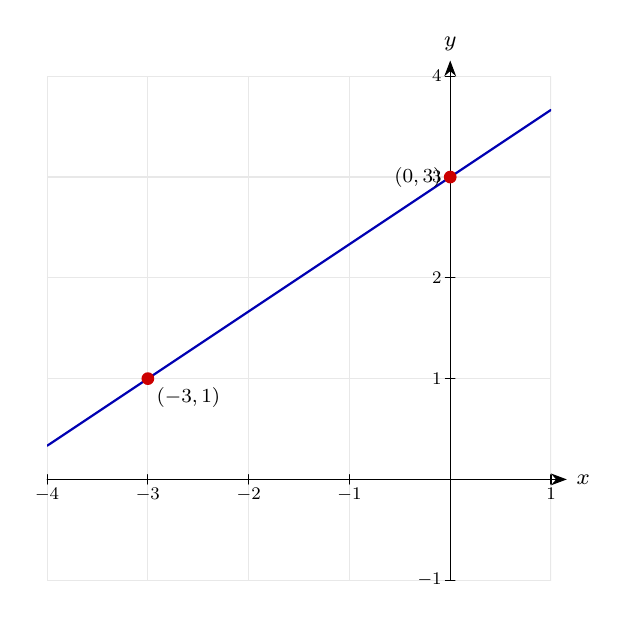
\begin{tikzpicture}[>={Stealth[length=2mm]},font=\footnotesize,line cap=round]
\begin{scope}
\clip (0,0) rectangle (6.4,6.4);
\draw[gray!18] (0,0) grid[xstep=1.28,ystep=1.28] (6.4,6.4);
\draw[blue!70!black,thick] (0,1.707) -- (6.4,5.973);
\end{scope}
\draw[->] (0,1.28) -- (6.6,1.28) node[right]{$x$};
\draw[->] (5.12,0) -- (5.12,6.6) node[above]{$y$};
\draw (0,1.22) -- (0,1.34) node[below=2pt,scale=0.8]{$-4$};
\draw (1.28,1.22) -- (1.28,1.34) node[below=2pt,scale=0.8]{$-3$};
\draw (2.56,1.22) -- (2.56,1.34) node[below=2pt,scale=0.8]{$-2$};
\draw (3.84,1.22) -- (3.84,1.34) node[below=2pt,scale=0.8]{$-1$};
\draw (6.4,1.22) -- (6.4,1.34) node[below=2pt,scale=0.8]{$1$};
\draw (5.06,0) -- (5.18,0) node[left=2pt,scale=0.8]{$-1$};
\draw (5.06,2.56) -- (5.18,2.56) node[left=2pt,scale=0.8]{$1$};
\draw (5.06,3.84) -- (5.18,3.84) node[left=2pt,scale=0.8]{$2$};
\draw (5.06,5.12) -- (5.18,5.12) node[left=2pt,scale=0.8]{$3$};
\draw (5.06,6.4) -- (5.18,6.4) node[left=2pt,scale=0.8]{$4$};
\fill[red!80!black] (1.28,2.56) circle (2.3pt);
\node[below right,scale=0.9] at (1.28,2.56) {$(-3,1)$};
\fill[red!80!black] (5.12,5.12) circle (2.3pt);
\node[left,scale=0.9] at (5.12,5.12) {$(0,3)$};
\end{tikzpicture}
}
\end{center}
\small The line(s) and key points shown on the coordinate plane.\normalsize

\medskip\hrule

\section*{Equation of a Straight Line 40\quad\small\texttt{(cg1-040)}}
\addcontentsline{toc}{section}{Equation of a Straight Line 40 (cg1-040)}
\textit{Difficulty: Foundation \quad\textbar\quad Marks: 3}

\question{Find the equation of the line through \( (0, -2) \) and \( (4, 6) \). Give your answer in the form \( ax + by + c = 0 \).}

\textbf{Worked solution.}

\textit{Step 1: Find gradient}
\[\begin{gathered}
m = \frac{6 - (-2)}{4 - 0} = \frac{8}{4} = 2
\end{gathered}\]
Either point can be used in the gradient formula.

\textit{Step 2: Equation}
\[\begin{gathered}
y = 2x - 2 \quad\quad \Rightarrow \quad\quad 2x - y - 2 = 0
\end{gathered}\]
Rearrange to standard form.

\begin{answerbox}
\textbf{Final answer:}\quad \(\displaystyle 2x - y - 2 = 0\) or equivalently \(\displaystyle -2x + y + 2 = 0\)
\end{answerbox}
\textbf{Common mistake.} Both forms are equally valid. Multiplying through by \(-1\) gives the other form.

\textbf{Diagram.}

\begin{center}
\resizebox{\ifdim\width>\linewidth \linewidth\else \width\fi}{!}{%
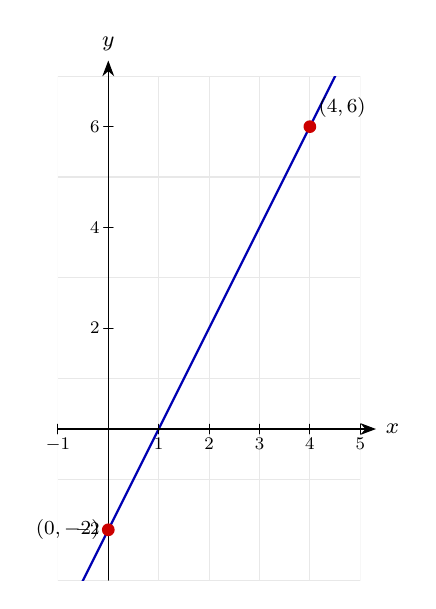
\begin{tikzpicture}[>={Stealth[length=2mm]},font=\footnotesize,line cap=round]
\begin{scope}
\clip (0,0) rectangle (3.84,6.4);
\draw[gray!18] (0,-0.64) grid[xstep=0.64,ystep=1.28] (3.84,6.4);
\draw[blue!70!black,thick] (0,-0.64) -- (3.84,7.04);
\end{scope}
\draw[->] (0,1.92) -- (4.04,1.92) node[right]{$x$};
\draw[->] (0.64,0) -- (0.64,6.6) node[above]{$y$};
\draw (0,1.86) -- (0,1.98) node[below=2pt,scale=0.8]{$-1$};
\draw (1.28,1.86) -- (1.28,1.98) node[below=2pt,scale=0.8]{$1$};
\draw (1.92,1.86) -- (1.92,1.98) node[below=2pt,scale=0.8]{$2$};
\draw (2.56,1.86) -- (2.56,1.98) node[below=2pt,scale=0.8]{$3$};
\draw (3.2,1.86) -- (3.2,1.98) node[below=2pt,scale=0.8]{$4$};
\draw (3.84,1.86) -- (3.84,1.98) node[below=2pt,scale=0.8]{$5$};
\draw (0.58,0.64) -- (0.7,0.64) node[left=2pt,scale=0.8]{$-2$};
\draw (0.58,3.2) -- (0.7,3.2) node[left=2pt,scale=0.8]{$2$};
\draw (0.58,4.48) -- (0.7,4.48) node[left=2pt,scale=0.8]{$4$};
\draw (0.58,5.76) -- (0.7,5.76) node[left=2pt,scale=0.8]{$6$};
\fill[red!80!black] (0.64,0.64) circle (2.3pt);
\node[left,scale=0.9] at (0.64,0.64) {$(0,-2)$};
\fill[red!80!black] (3.2,5.76) circle (2.3pt);
\node[above right,scale=0.9] at (3.2,5.76) {$(4,6)$};
\end{tikzpicture}
}
\end{center}
\small The line(s) and key points shown on the coordinate plane.\normalsize

\medskip\hrule

\section*{Equation of a Straight Line 41\quad\small\texttt{(cg1-041)}}
\addcontentsline{toc}{section}{Equation of a Straight Line 41 (cg1-041)}
\textit{Difficulty: Foundation \quad\textbar\quad Marks: 2}

\question{Find the midpoint of \( A(3, -1) \) and \( B(7, 5) \).}

\textbf{Worked solution.}

\textit{Apply midpoint formula}
\[\begin{gathered}
M = \left(\frac{3+7}{2}, \frac{-1+5}{2}\right) = (5, 2)
\end{gathered}\]
Average the coordinates.

\begin{answerbox}
\textbf{Final answer:}\quad \(\displaystyle (5, 2)\)
\end{answerbox}
\textbf{Diagram.}

\begin{center}
\resizebox{\ifdim\width>\linewidth \linewidth\else \width\fi}{!}{%
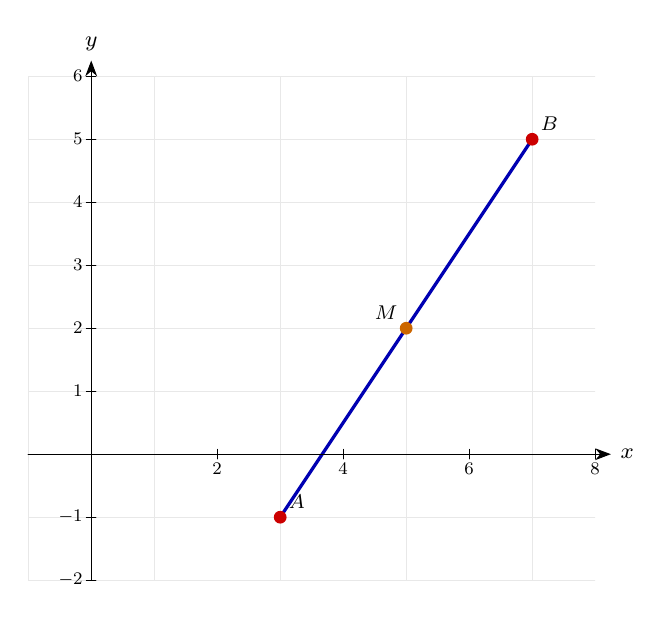
\begin{tikzpicture}[>={Stealth[length=2mm]},font=\footnotesize,line cap=round]
\begin{scope}
\clip (0,0) rectangle (7.2,6.4);
\draw[gray!18] (-0.8,0) grid[xstep=1.6,ystep=0.8] (7.2,6.4);
\draw[blue!70!black,very thick] (3.2,0.8) -- (6.4,5.6);
\end{scope}
\draw[->] (0,1.6) -- (7.4,1.6) node[right]{$x$};
\draw[->] (0.8,0) -- (0.8,6.6) node[above]{$y$};
\draw (2.4,1.54) -- (2.4,1.66) node[below=2pt,scale=0.8]{$2$};
\draw (4,1.54) -- (4,1.66) node[below=2pt,scale=0.8]{$4$};
\draw (5.6,1.54) -- (5.6,1.66) node[below=2pt,scale=0.8]{$6$};
\draw (7.2,1.54) -- (7.2,1.66) node[below=2pt,scale=0.8]{$8$};
\draw (0.74,0) -- (0.86,0) node[left=2pt,scale=0.8]{$-2$};
\draw (0.74,0.8) -- (0.86,0.8) node[left=2pt,scale=0.8]{$-1$};
\draw (0.74,2.4) -- (0.86,2.4) node[left=2pt,scale=0.8]{$1$};
\draw (0.74,3.2) -- (0.86,3.2) node[left=2pt,scale=0.8]{$2$};
\draw (0.74,4) -- (0.86,4) node[left=2pt,scale=0.8]{$3$};
\draw (0.74,4.8) -- (0.86,4.8) node[left=2pt,scale=0.8]{$4$};
\draw (0.74,5.6) -- (0.86,5.6) node[left=2pt,scale=0.8]{$5$};
\draw (0.74,6.4) -- (0.86,6.4) node[left=2pt,scale=0.8]{$6$};
\fill[red!80!black] (3.2,0.8) circle (2.3pt);
\node[above right,scale=0.9] at (3.2,0.8) {$A$};
\fill[red!80!black] (6.4,5.6) circle (2.3pt);
\node[above right,scale=0.9] at (6.4,5.6) {$B$};
\fill[orange!80!black] (4.8,3.2) circle (2.3pt);
\node[above left,scale=0.9] at (4.8,3.2) {$M$};
\end{tikzpicture}
}
\end{center}
\small The line(s) and key points shown on the coordinate plane.\normalsize

\medskip\hrule

\section*{Equation of a Straight Line 42\quad\small\texttt{(cg1-042)}}
\addcontentsline{toc}{section}{Equation of a Straight Line 42 (cg1-042)}
\textit{Difficulty: Foundation \quad\textbar\quad Marks: 2}

\question{Find the distance between \( P(1, 3) \) and \( Q(4, 7) \).}

\textbf{Worked solution.}

\textit{Apply distance formula}
\[\begin{gathered}
PQ = \sqrt{(4-1)^2 + (7-3)^2} = \sqrt{9 + 16} = \sqrt{25} = 5
\end{gathered}\]
The distance formula \(d = \sqrt{(x_2 - x_1)^2 + (y_2 - y_1)^2}\) is Pythagoras applied to the horizontal and vertical separations between the points.

\begin{answerbox}
\textbf{Final answer:}\quad \(\displaystyle 5\)
\end{answerbox}
\textbf{Diagram.}

\begin{center}
\resizebox{\ifdim\width>\linewidth \linewidth\else \width\fi}{!}{%
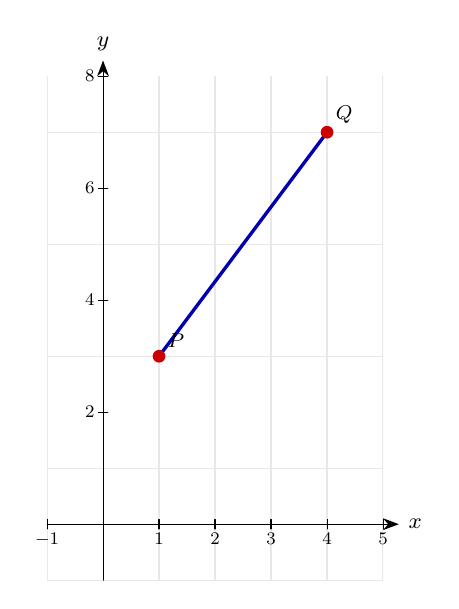
\begin{tikzpicture}[>={Stealth[length=2mm]},font=\footnotesize,line cap=round]
\begin{scope}
\clip (0,0) rectangle (4.267,6.4);
\draw[gray!18] (0,-0.711) grid[xstep=0.711,ystep=1.422] (4.267,6.4);
\draw[blue!70!black,very thick] (1.422,2.844) -- (3.556,5.689);
\end{scope}
\draw[->] (0,0.711) -- (4.467,0.711) node[right]{$x$};
\draw[->] (0.711,0) -- (0.711,6.6) node[above]{$y$};
\draw (0,0.651) -- (0,0.771) node[below=2pt,scale=0.8]{$-1$};
\draw (1.422,0.651) -- (1.422,0.771) node[below=2pt,scale=0.8]{$1$};
\draw (2.133,0.651) -- (2.133,0.771) node[below=2pt,scale=0.8]{$2$};
\draw (2.844,0.651) -- (2.844,0.771) node[below=2pt,scale=0.8]{$3$};
\draw (3.556,0.651) -- (3.556,0.771) node[below=2pt,scale=0.8]{$4$};
\draw (4.267,0.651) -- (4.267,0.771) node[below=2pt,scale=0.8]{$5$};
\draw (0.651,2.133) -- (0.771,2.133) node[left=2pt,scale=0.8]{$2$};
\draw (0.651,3.556) -- (0.771,3.556) node[left=2pt,scale=0.8]{$4$};
\draw (0.651,4.978) -- (0.771,4.978) node[left=2pt,scale=0.8]{$6$};
\draw (0.651,6.4) -- (0.771,6.4) node[left=2pt,scale=0.8]{$8$};
\fill[red!80!black] (1.422,2.844) circle (2.3pt);
\node[above right,scale=0.9] at (1.422,2.844) {$P$};
\fill[red!80!black] (3.556,5.689) circle (2.3pt);
\node[above right,scale=0.9] at (3.556,5.689) {$Q$};
\end{tikzpicture}
}
\end{center}
\small The line(s) and key points shown on the coordinate plane.\normalsize

\medskip\hrule

\section*{Equation of a Straight Line 43\quad\small\texttt{(cg1-043)}}
\addcontentsline{toc}{section}{Equation of a Straight Line 43 (cg1-043)}
\textit{Difficulty: Foundation \quad\textbar\quad Marks: 2}

\question{The line \( L \) passes through \( (1, 4) \) and is parallel to \( y = 2x - 3 \). Find the equation of \( L \).}

\textbf{Worked solution.}

\textit{Step 1: Parallel lines have equal gradients}
\[\begin{gathered}
m = 2
\end{gathered}\]
Same gradient as y = 2x - 3.

\textit{Step 2: Use point-slope}
\[\begin{gathered}
y - 4 = 2(x - 1) \implies y = 2x + 2
\end{gathered}\]
Substitute the gradient and the point \((1, 4)\) into \(y - y_1 = m(x - x_1)\), then expand and simplify.

\begin{answerbox}
\textbf{Final answer:}\quad \(\displaystyle y = 2x + 2\)
\end{answerbox}
\textbf{Diagram.}

\begin{center}
\resizebox{\ifdim\width>\linewidth \linewidth\else \width\fi}{!}{%
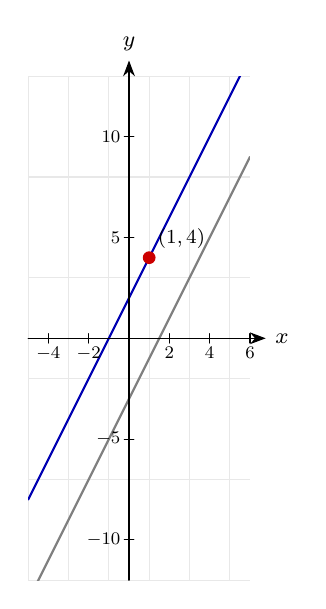
\begin{tikzpicture}[>={Stealth[length=2mm]},font=\footnotesize,line cap=round]
\begin{scope}
\clip (0,0) rectangle (2.816,6.4);
\draw[gray!18] (-0.256,-0.768) grid[xstep=0.512,ystep=1.28] (2.816,6.4);
\draw[gray,thick] (0,-0.256) -- (2.816,5.376);
\draw[blue!70!black,thick] (0,1.024) -- (2.816,6.656);
\end{scope}
\draw[->] (0,3.072) -- (3.016,3.072) node[right]{$x$};
\draw[->] (1.28,0) -- (1.28,6.6) node[above]{$y$};
\draw (0.256,3.012) -- (0.256,3.132) node[below=2pt,scale=0.8]{$-4$};
\draw (0.768,3.012) -- (0.768,3.132) node[below=2pt,scale=0.8]{$-2$};
\draw (1.792,3.012) -- (1.792,3.132) node[below=2pt,scale=0.8]{$2$};
\draw (2.304,3.012) -- (2.304,3.132) node[below=2pt,scale=0.8]{$4$};
\draw (2.816,3.012) -- (2.816,3.132) node[below=2pt,scale=0.8]{$6$};
\draw (1.22,0.512) -- (1.34,0.512) node[left=2pt,scale=0.8]{$-10$};
\draw (1.22,1.792) -- (1.34,1.792) node[left=2pt,scale=0.8]{$-5$};
\draw (1.22,4.352) -- (1.34,4.352) node[left=2pt,scale=0.8]{$5$};
\draw (1.22,5.632) -- (1.34,5.632) node[left=2pt,scale=0.8]{$10$};
\fill[red!80!black] (1.536,4.096) circle (2.3pt);
\node[above right,scale=0.9] at (1.536,4.096) {$(1,4)$};
\end{tikzpicture}
}
\end{center}
\small The line(s) and key points shown on the coordinate plane.\normalsize

\medskip\hrule

\section*{Equation of a Straight Line 44\quad\small\texttt{(cg1-044)}}
\addcontentsline{toc}{section}{Equation of a Straight Line 44 (cg1-044)}
\textit{Difficulty: Foundation \quad\textbar\quad Marks: 3}

\question{The line \( L \) passes through \( (3, 1) \) and is perpendicular to \( y = \frac{1}{2}x + 5 \). Find the equation of \( L \).}

\textbf{Worked solution.}

\textit{Step 1: Perpendicular gradient}
\[\begin{gathered}
m = -\frac{1}{\frac{1}{2}} = -2
\end{gathered}\]
Negative reciprocal.

\textit{Step 2: Equation}
\[\begin{gathered}
y - 1 = -2(x - 3) \implies y = -2x + 7
\end{gathered}\]
Substitute the perpendicular gradient and \((3, 1)\) into \(y - y_1 = m(x - x_1)\), then expand: \(-2(x-3) = -2x + 6\), and add 1.

\begin{answerbox}
\textbf{Final answer:}\quad \(\displaystyle y = -2x + 7\)
\end{answerbox}
\textbf{Diagram.}

\begin{center}
\resizebox{\ifdim\width>\linewidth \linewidth\else \width\fi}{!}{%
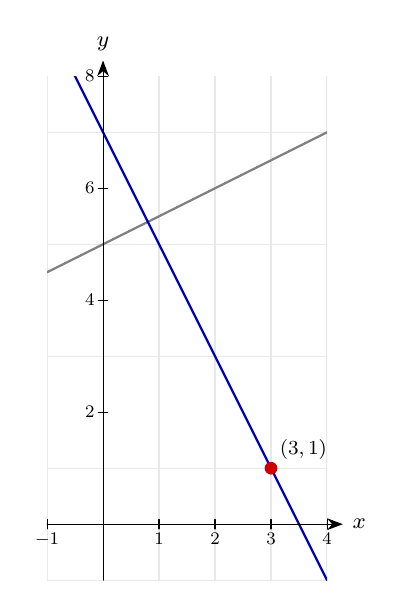
\begin{tikzpicture}[>={Stealth[length=2mm]},font=\footnotesize,line cap=round]
\begin{scope}
\clip (0,0) rectangle (3.556,6.4);
\draw[gray!18] (0,-0.711) grid[xstep=0.711,ystep=1.422] (3.556,6.4);
\draw[gray,thick] (0,3.911) -- (3.556,5.689);
\draw[blue!70!black,thick] (0,7.111) -- (3.556,0);
\end{scope}
\draw[->] (0,0.711) -- (3.756,0.711) node[right]{$x$};
\draw[->] (0.711,0) -- (0.711,6.6) node[above]{$y$};
\draw (0,0.651) -- (0,0.771) node[below=2pt,scale=0.8]{$-1$};
\draw (1.422,0.651) -- (1.422,0.771) node[below=2pt,scale=0.8]{$1$};
\draw (2.133,0.651) -- (2.133,0.771) node[below=2pt,scale=0.8]{$2$};
\draw (2.844,0.651) -- (2.844,0.771) node[below=2pt,scale=0.8]{$3$};
\draw (3.556,0.651) -- (3.556,0.771) node[below=2pt,scale=0.8]{$4$};
\draw (0.651,2.133) -- (0.771,2.133) node[left=2pt,scale=0.8]{$2$};
\draw (0.651,3.556) -- (0.771,3.556) node[left=2pt,scale=0.8]{$4$};
\draw (0.651,4.978) -- (0.771,4.978) node[left=2pt,scale=0.8]{$6$};
\draw (0.651,6.4) -- (0.771,6.4) node[left=2pt,scale=0.8]{$8$};
\fill[red!80!black] (2.844,1.422) circle (2.3pt);
\node[above right,scale=0.9] at (2.844,1.422) {$(3,1)$};
\end{tikzpicture}
}
\end{center}
\small The line(s) and key points shown on the coordinate plane.\normalsize

\medskip\hrule

\section*{Equation of a Straight Line 45\quad\small\texttt{(cg1-045)}}
\addcontentsline{toc}{section}{Equation of a Straight Line 45 (cg1-045)}
\textit{Difficulty: Foundation \quad\textbar\quad Marks: 3}

\question{Find where the lines \( y = 3x - 1 \) and \( y = -x + 7 \) intersect.}

\textbf{Worked solution.}

\textit{Step 1: Set equal}
\[\begin{gathered}
3x - 1 = -x + 7 \implies 4x = 8 \implies x = 2
\end{gathered}\]
At the intersection both lines share the same \(y\), so setting the right-hand sides equal gives an equation for the \(x\)-coordinate.

\textit{Step 2: Find y}
\[\begin{gathered}
y = 3(2) - 1 = 5
\end{gathered}\]
Substitute back into either line --- both will give the same \(y\) at the intersection point.

\begin{answerbox}
\textbf{Final answer:}\quad \(\displaystyle (2, 5)\)
\end{answerbox}
\textbf{Diagram.}

\begin{center}
\resizebox{\ifdim\width>\linewidth \linewidth\else \width\fi}{!}{%
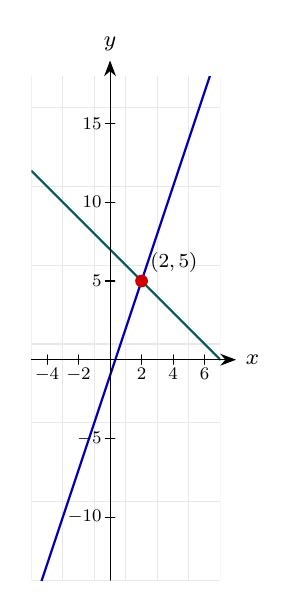
\begin{tikzpicture}[>={Stealth[length=2mm]},font=\footnotesize,line cap=round]
\begin{scope}
\clip (0,0) rectangle (2.4,6.4);
\draw[gray!18] (-0.2,-0.2) grid[xstep=0.4,ystep=1] (2.4,6.4);
\draw[blue!70!black,thick] (0,-0.4) -- (2.4,6.8);
\draw[teal!70!black,thick] (0,5.2) -- (2.4,2.8);
\end{scope}
\draw[->] (0,2.8) -- (2.6,2.8) node[right]{$x$};
\draw[->] (1,0) -- (1,6.6) node[above]{$y$};
\draw (0.2,2.74) -- (0.2,2.86) node[below=2pt,scale=0.8]{$-4$};
\draw (0.6,2.74) -- (0.6,2.86) node[below=2pt,scale=0.8]{$-2$};
\draw (1.4,2.74) -- (1.4,2.86) node[below=2pt,scale=0.8]{$2$};
\draw (1.8,2.74) -- (1.8,2.86) node[below=2pt,scale=0.8]{$4$};
\draw (2.2,2.74) -- (2.2,2.86) node[below=2pt,scale=0.8]{$6$};
\draw (0.94,0.8) -- (1.06,0.8) node[left=2pt,scale=0.8]{$-10$};
\draw (0.94,1.8) -- (1.06,1.8) node[left=2pt,scale=0.8]{$-5$};
\draw (0.94,3.8) -- (1.06,3.8) node[left=2pt,scale=0.8]{$5$};
\draw (0.94,4.8) -- (1.06,4.8) node[left=2pt,scale=0.8]{$10$};
\draw (0.94,5.8) -- (1.06,5.8) node[left=2pt,scale=0.8]{$15$};
\fill[red!80!black] (1.4,3.8) circle (2.3pt);
\node[above right,scale=0.9] at (1.4,3.8) {$(2,5)$};
\end{tikzpicture}
}
\end{center}
\small The line(s) and key points shown on the coordinate plane.\normalsize

\medskip\hrule

\section*{Equation of a Straight Line 46\quad\small\texttt{(cg1-046)}}
\addcontentsline{toc}{section}{Equation of a Straight Line 46 (cg1-046)}
\textit{Difficulty: Foundation \quad\textbar\quad Marks: 3}

\question{Show that the points \( A(1, 2) \), \( B(3, 6) \) and \( C(5, 10) \) are collinear.}

\textbf{Worked solution.}

\textit{Step 1: Gradient AB}
\[\begin{gathered}
m_{AB} = \frac{6-2}{3-1} = 2
\end{gathered}\]
To show three points are collinear, we check that two segments through a common point share the same gradient.

\textit{Step 2: Gradient BC}
\[\begin{gathered}
m_{BC} = \frac{10-6}{5-3} = 2
\end{gathered}\]
Equal gradients and shared point B means collinear.

\begin{answerbox}
\textbf{Final answer:}\quad Gradients are equal so A, B, C are collinear.
\end{answerbox}
\textbf{Diagram.}

\begin{center}
\resizebox{\ifdim\width>\linewidth \linewidth\else \width\fi}{!}{%
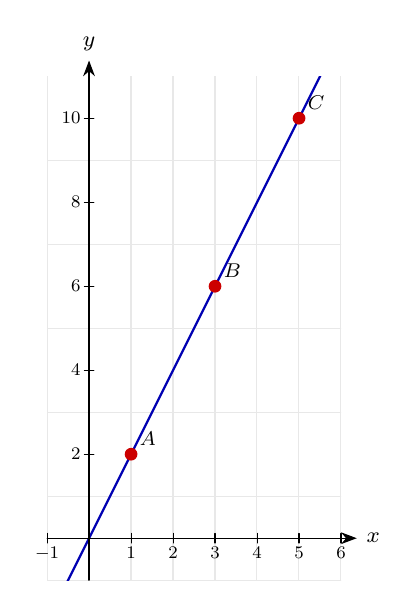
\begin{tikzpicture}[>={Stealth[length=2mm]},font=\footnotesize,line cap=round]
\begin{scope}
\clip (0,0) rectangle (3.733,6.4);
\draw[gray!18] (0,-0.533) grid[xstep=0.533,ystep=1.067] (3.733,6.4);
\draw[blue!70!black,thick] (0,-0.533) -- (3.733,6.933);
\end{scope}
\draw[->] (0,0.533) -- (3.933,0.533) node[right]{$x$};
\draw[->] (0.533,0) -- (0.533,6.6) node[above]{$y$};
\draw (0,0.473) -- (0,0.593) node[below=2pt,scale=0.8]{$-1$};
\draw (1.067,0.473) -- (1.067,0.593) node[below=2pt,scale=0.8]{$1$};
\draw (1.6,0.473) -- (1.6,0.593) node[below=2pt,scale=0.8]{$2$};
\draw (2.133,0.473) -- (2.133,0.593) node[below=2pt,scale=0.8]{$3$};
\draw (2.667,0.473) -- (2.667,0.593) node[below=2pt,scale=0.8]{$4$};
\draw (3.2,0.473) -- (3.2,0.593) node[below=2pt,scale=0.8]{$5$};
\draw (3.733,0.473) -- (3.733,0.593) node[below=2pt,scale=0.8]{$6$};
\draw (0.473,1.6) -- (0.593,1.6) node[left=2pt,scale=0.8]{$2$};
\draw (0.473,2.667) -- (0.593,2.667) node[left=2pt,scale=0.8]{$4$};
\draw (0.473,3.733) -- (0.593,3.733) node[left=2pt,scale=0.8]{$6$};
\draw (0.473,4.8) -- (0.593,4.8) node[left=2pt,scale=0.8]{$8$};
\draw (0.473,5.867) -- (0.593,5.867) node[left=2pt,scale=0.8]{$10$};
\fill[red!80!black] (1.067,1.6) circle (2.3pt);
\node[above right,scale=0.9] at (1.067,1.6) {$A$};
\fill[red!80!black] (2.133,3.733) circle (2.3pt);
\node[above right,scale=0.9] at (2.133,3.733) {$B$};
\fill[red!80!black] (3.2,5.867) circle (2.3pt);
\node[above right,scale=0.9] at (3.2,5.867) {$C$};
\end{tikzpicture}
}
\end{center}
\small The line(s) and key points shown on the coordinate plane.\normalsize

\medskip\hrule

\section*{Equation of a Straight Line 47\quad\small\texttt{(cg1-047)}}
\addcontentsline{toc}{section}{Equation of a Straight Line 47 (cg1-047)}
\textit{Difficulty: Foundation \quad\textbar\quad Marks: 4}

\question{Find the equation of the perpendicular bisector of the line segment joining \( A(2, 4) \) and \( B(6, 0) \).}

\textbf{Worked solution.}

\textit{Step 1: Midpoint}
\[\begin{gathered}
M = (4, 2)
\end{gathered}\]
The perpendicular bisector passes through the midpoint of \(AB\): average the coordinates to get \(\left(\tfrac{2+6}{2}, \tfrac{4+0}{2}\right) = (4, 2)\).

\textit{Step 2: Gradient of AB}
\[\begin{gathered}
m_{AB} = \frac{0-4}{6-2} = -1
\end{gathered}\]
We need the gradient of \(AB\) so we can take its negative reciprocal to get the perpendicular gradient.

\textit{Step 3: Perpendicular gradient and equation}
\[\begin{gathered}
m_{\perp} = 1; \quad y - 2 = 1(x - 4) \implies y = x - 2
\end{gathered}\]
Perpendicular gradients satisfy \(m_1 m_2 = -1\), so the negative reciprocal of \(-1\) is \(1\). Substitute into \(y - y_1 = m(x - x_1)\) using the midpoint.

\begin{answerbox}
\textbf{Final answer:}\quad \(\displaystyle y = x - 2\)
\end{answerbox}
\textbf{Diagram.}

\begin{center}
\resizebox{\ifdim\width>\linewidth \linewidth\else \width\fi}{!}{%
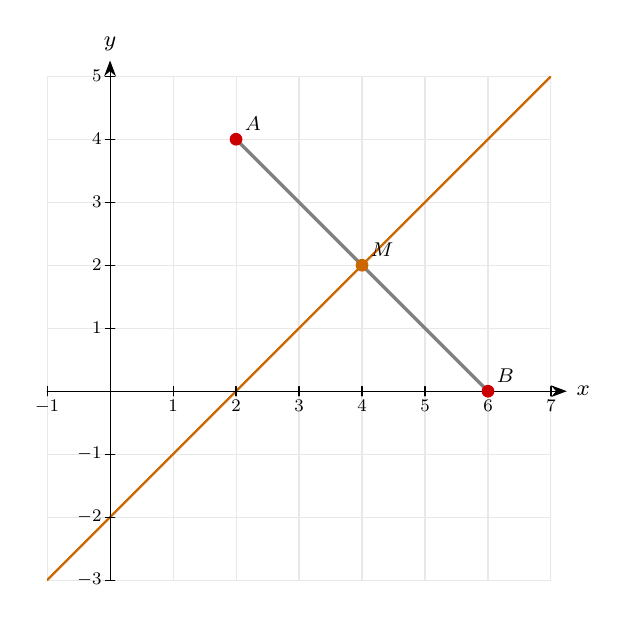
\begin{tikzpicture}[>={Stealth[length=2mm]},font=\footnotesize,line cap=round]
\begin{scope}
\clip (0,0) rectangle (6.4,6.4);
\draw[gray!18] (0,0) grid[xstep=0.8,ystep=0.8] (6.4,6.4);
\draw[orange!80!black,thick] (0,0) -- (6.4,6.4);
\draw[gray,very thick] (2.4,5.6) -- (5.6,2.4);
\end{scope}
\draw[->] (0,2.4) -- (6.6,2.4) node[right]{$x$};
\draw[->] (0.8,0) -- (0.8,6.6) node[above]{$y$};
\draw (0,2.34) -- (0,2.46) node[below=2pt,scale=0.8]{$-1$};
\draw (1.6,2.34) -- (1.6,2.46) node[below=2pt,scale=0.8]{$1$};
\draw (2.4,2.34) -- (2.4,2.46) node[below=2pt,scale=0.8]{$2$};
\draw (3.2,2.34) -- (3.2,2.46) node[below=2pt,scale=0.8]{$3$};
\draw (4,2.34) -- (4,2.46) node[below=2pt,scale=0.8]{$4$};
\draw (4.8,2.34) -- (4.8,2.46) node[below=2pt,scale=0.8]{$5$};
\draw (5.6,2.34) -- (5.6,2.46) node[below=2pt,scale=0.8]{$6$};
\draw (6.4,2.34) -- (6.4,2.46) node[below=2pt,scale=0.8]{$7$};
\draw (0.74,0) -- (0.86,0) node[left=2pt,scale=0.8]{$-3$};
\draw (0.74,0.8) -- (0.86,0.8) node[left=2pt,scale=0.8]{$-2$};
\draw (0.74,1.6) -- (0.86,1.6) node[left=2pt,scale=0.8]{$-1$};
\draw (0.74,3.2) -- (0.86,3.2) node[left=2pt,scale=0.8]{$1$};
\draw (0.74,4) -- (0.86,4) node[left=2pt,scale=0.8]{$2$};
\draw (0.74,4.8) -- (0.86,4.8) node[left=2pt,scale=0.8]{$3$};
\draw (0.74,5.6) -- (0.86,5.6) node[left=2pt,scale=0.8]{$4$};
\draw (0.74,6.4) -- (0.86,6.4) node[left=2pt,scale=0.8]{$5$};
\fill[red!80!black] (2.4,5.6) circle (2.3pt);
\node[above right,scale=0.9] at (2.4,5.6) {$A$};
\fill[red!80!black] (5.6,2.4) circle (2.3pt);
\node[above right,scale=0.9] at (5.6,2.4) {$B$};
\fill[orange!80!black] (4,4) circle (2.3pt);
\node[above right,scale=0.9] at (4,4) {$M$};
\end{tikzpicture}
}
\end{center}
\small The line(s) and key points shown on the coordinate plane.\normalsize

\medskip\hrule

\section*{Equation of a Straight Line 48\quad\small\texttt{(cg1-048)}}
\addcontentsline{toc}{section}{Equation of a Straight Line 48 (cg1-048)}
\textit{Difficulty: Foundation \quad\textbar\quad Marks: 3}

\question{A line passes through \( (-1, 5) \) with gradient \( -4 \). Find where it crosses the x-axis.}

\textbf{Worked solution.}

\textit{Step 1: Equation}
\[\begin{gathered}
y - 5 = -4(x + 1) \implies y = -4x + 1
\end{gathered}\]
Substitute the gradient and point into \(y - y_1 = m(x - x_1)\). Note \(x - (-1) = x + 1\), then \(-4 \cdot 1 + 5 = 1\) gives the intercept.

\textit{Step 2: Set y = 0}
\[\begin{gathered}
0 = -4x + 1 \implies x = \frac{1}{4}
\end{gathered}\]
A line meets the \(x\)-axis where \(y = 0\). Solving the resulting equation gives the \(x\)-intercept.

\begin{answerbox}
\textbf{Final answer:}\quad \(\displaystyle \left(\frac{1}{4}, 0\right)\)
\end{answerbox}
\textbf{Diagram.}

\begin{center}
\resizebox{\ifdim\width>\linewidth \linewidth\else \width\fi}{!}{%
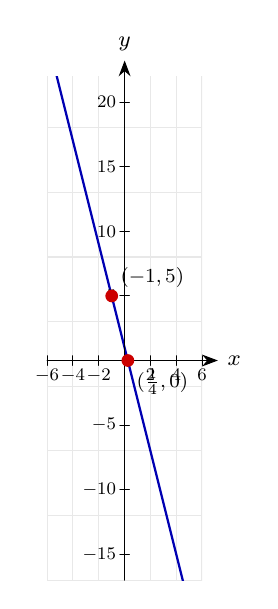
\begin{tikzpicture}[>={Stealth[length=2mm]},font=\footnotesize,line cap=round]
\begin{scope}
\clip (0,0) rectangle (1.969,6.4);
\draw[gray!18] (0,-0.492) grid[xstep=0.328,ystep=0.821] (1.969,6.4);
\draw[blue!70!black,thick] (0,6.892) -- (1.969,-0.985);
\end{scope}
\draw[->] (0,2.79) -- (2.169,2.79) node[right]{$x$};
\draw[->] (0.985,0) -- (0.985,6.6) node[above]{$y$};
\draw (0,2.73) -- (0,2.85) node[below=2pt,scale=0.8]{$-6$};
\draw (0.328,2.73) -- (0.328,2.85) node[below=2pt,scale=0.8]{$-4$};
\draw (0.656,2.73) -- (0.656,2.85) node[below=2pt,scale=0.8]{$-2$};
\draw (1.313,2.73) -- (1.313,2.85) node[below=2pt,scale=0.8]{$2$};
\draw (1.641,2.73) -- (1.641,2.85) node[below=2pt,scale=0.8]{$4$};
\draw (1.969,2.73) -- (1.969,2.85) node[below=2pt,scale=0.8]{$6$};
\draw (0.925,0.328) -- (1.045,0.328) node[left=2pt,scale=0.8]{$-15$};
\draw (0.925,1.149) -- (1.045,1.149) node[left=2pt,scale=0.8]{$-10$};
\draw (0.925,1.969) -- (1.045,1.969) node[left=2pt,scale=0.8]{$-5$};
\draw (0.925,3.61) -- (1.045,3.61) node[left=2pt,scale=0.8]{$5$};
\draw (0.925,4.431) -- (1.045,4.431) node[left=2pt,scale=0.8]{$10$};
\draw (0.925,5.251) -- (1.045,5.251) node[left=2pt,scale=0.8]{$15$};
\draw (0.925,6.072) -- (1.045,6.072) node[left=2pt,scale=0.8]{$20$};
\fill[red!80!black] (0.821,3.61) circle (2.3pt);
\node[above right,scale=0.9] at (0.821,3.61) {$(-1,5)$};
\fill[red!80!black] (1.026,2.79) circle (2.3pt);
\node[below right,scale=0.9] at (1.026,2.79) {$(\tfrac14,0)$};
\end{tikzpicture}
}
\end{center}
\small The line(s) and key points shown on the coordinate plane.\normalsize

\medskip\hrule

\section*{Equation of a Straight Line 49\quad\small\texttt{(cg1-049)}}
\addcontentsline{toc}{section}{Equation of a Straight Line 49 (cg1-049)}
\textit{Difficulty: Foundation \quad\textbar\quad Marks: 3}

\question{Find the value of \( k \) if the line through \( (2, 3) \) and \( (k, 7) \) has gradient \( \frac{4}{3} \).}

\textbf{Worked solution.}

\textit{Step 1: Set up gradient equation}
\[\begin{gathered}
\frac{7-3}{k-2} = \frac{4}{3}
\end{gathered}\]
Apply \(m = \frac{y_2 - y_1}{x_2 - x_1}\) and equate to the given gradient --- this gives an equation we can solve for \(k\).

\textit{Step 2: Solve}
\[\begin{gathered}
\frac{4}{k-2} = \frac{4}{3} \implies k - 2 = 3 \implies k = 5
\end{gathered}\]
Since the numerators are equal, the denominators must be equal too. (Equivalently, cross-multiply.)

\begin{answerbox}
\textbf{Final answer:}\quad \(\displaystyle k = 5\)
\end{answerbox}
\textbf{Diagram.}

\begin{center}
\resizebox{\ifdim\width>\linewidth \linewidth\else \width\fi}{!}{%
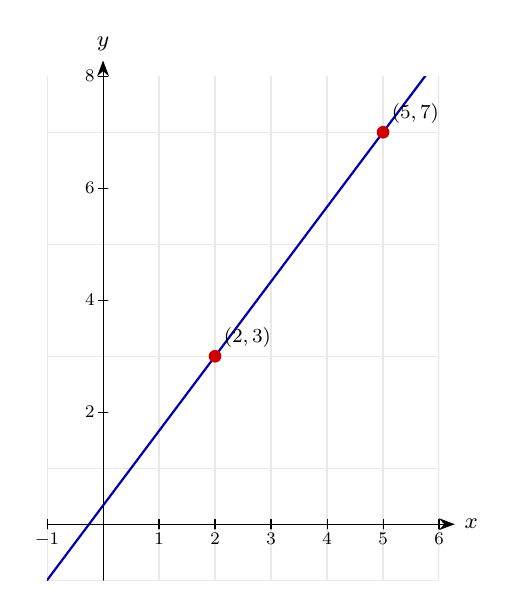
\begin{tikzpicture}[>={Stealth[length=2mm]},font=\footnotesize,line cap=round]
\begin{scope}
\clip (0,0) rectangle (4.978,6.4);
\draw[gray!18] (0,-0.711) grid[xstep=0.711,ystep=1.422] (4.978,6.4);
\draw[blue!70!black,thick] (0,0) -- (4.978,6.637);
\end{scope}
\draw[->] (0,0.711) -- (5.178,0.711) node[right]{$x$};
\draw[->] (0.711,0) -- (0.711,6.6) node[above]{$y$};
\draw (0,0.651) -- (0,0.771) node[below=2pt,scale=0.8]{$-1$};
\draw (1.422,0.651) -- (1.422,0.771) node[below=2pt,scale=0.8]{$1$};
\draw (2.133,0.651) -- (2.133,0.771) node[below=2pt,scale=0.8]{$2$};
\draw (2.844,0.651) -- (2.844,0.771) node[below=2pt,scale=0.8]{$3$};
\draw (3.556,0.651) -- (3.556,0.771) node[below=2pt,scale=0.8]{$4$};
\draw (4.267,0.651) -- (4.267,0.771) node[below=2pt,scale=0.8]{$5$};
\draw (4.978,0.651) -- (4.978,0.771) node[below=2pt,scale=0.8]{$6$};
\draw (0.651,2.133) -- (0.771,2.133) node[left=2pt,scale=0.8]{$2$};
\draw (0.651,3.556) -- (0.771,3.556) node[left=2pt,scale=0.8]{$4$};
\draw (0.651,4.978) -- (0.771,4.978) node[left=2pt,scale=0.8]{$6$};
\draw (0.651,6.4) -- (0.771,6.4) node[left=2pt,scale=0.8]{$8$};
\fill[red!80!black] (2.133,2.844) circle (2.3pt);
\node[above right,scale=0.9] at (2.133,2.844) {$(2,3)$};
\fill[red!80!black] (4.267,5.689) circle (2.3pt);
\node[above right,scale=0.9] at (4.267,5.689) {$(5,7)$};
\end{tikzpicture}
}
\end{center}
\small The line(s) and key points shown on the coordinate plane.\normalsize

\medskip\hrule

\section*{Equation of a Straight Line 50\quad\small\texttt{(cg1-050)}}
\addcontentsline{toc}{section}{Equation of a Straight Line 50 (cg1-050)}
\textit{Difficulty: Foundation \quad\textbar\quad Marks: 4}

\question{The line \( 3x - 2y + 6 = 0 \) meets the x-axis at \( A \) and the y-axis at \( B \). Find the area of triangle \( OAB \).}

\textbf{Worked solution.}

\textit{Step 1: Find A (y=0)}
\[\begin{gathered}
3x + 6 = 0 \implies x = -2, \quad A = (-2, 0)
\end{gathered}\]
A line crosses the \(x\)-axis where \(y = 0\). Set \(y = 0\) in the equation and solve for \(x\).

\textit{Step 2: Find B (x=0)}
\[\begin{gathered}
-2y + 6 = 0 \implies y = 3, \quad B = (0, 3)
\end{gathered}\]
A line crosses the \(y\)-axis where \(x = 0\). Set \(x = 0\) in the equation and solve for \(y\).

\textit{Step 3: Area}
\[\begin{gathered}
\text{Area} = \frac{1}{2} \times 2 \times 3 = 3
\end{gathered}\]
Base = 2, height = 3.

\begin{answerbox}
\textbf{Final answer:}\quad \(\displaystyle 3\) square units
\end{answerbox}
\textbf{Diagram.}

\begin{center}
\resizebox{\ifdim\width>\linewidth \linewidth\else \width\fi}{!}{%
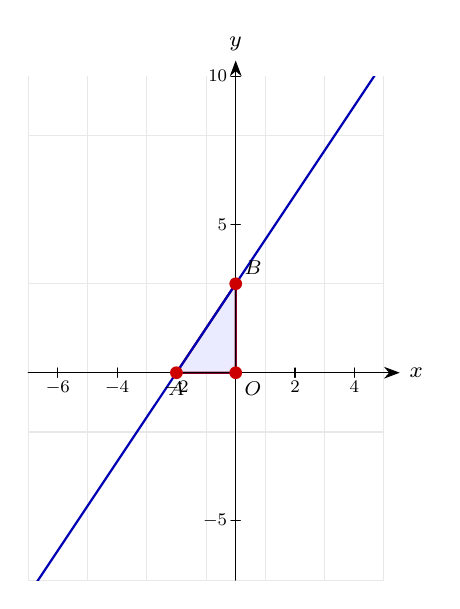
\begin{tikzpicture}[>={Stealth[length=2mm]},font=\footnotesize,line cap=round]
\begin{scope}
\clip (0,0) rectangle (4.518,6.4);
\draw[gray!18] (-0.376,-1.129) grid[xstep=0.753,ystep=1.882] (4.518,6.4);
\fill[blue!8] (2.635,2.635) -- (1.882,2.635) -- (2.635,3.765) -- cycle;
\draw[purple!70!black,thick] (2.635,2.635) -- (1.882,2.635) -- (2.635,3.765) -- cycle;
\draw[blue!70!black,thick] (0,-0.188) -- (4.518,6.588);
\end{scope}
\draw[->] (0,2.635) -- (4.718,2.635) node[right]{$x$};
\draw[->] (2.635,0) -- (2.635,6.6) node[above]{$y$};
\draw (0.376,2.575) -- (0.376,2.695) node[below=2pt,scale=0.8]{$-6$};
\draw (1.129,2.575) -- (1.129,2.695) node[below=2pt,scale=0.8]{$-4$};
\draw (1.882,2.575) -- (1.882,2.695) node[below=2pt,scale=0.8]{$-2$};
\draw (3.388,2.575) -- (3.388,2.695) node[below=2pt,scale=0.8]{$2$};
\draw (4.141,2.575) -- (4.141,2.695) node[below=2pt,scale=0.8]{$4$};
\draw (2.575,0.753) -- (2.695,0.753) node[left=2pt,scale=0.8]{$-5$};
\draw (2.575,4.518) -- (2.695,4.518) node[left=2pt,scale=0.8]{$5$};
\draw (2.575,6.4) -- (2.695,6.4) node[left=2pt,scale=0.8]{$10$};
\fill[red!80!black] (2.635,2.635) circle (2.3pt);
\node[below right,scale=0.9] at (2.635,2.635) {$O$};
\fill[red!80!black] (1.882,2.635) circle (2.3pt);
\node[below,scale=0.9] at (1.882,2.635) {$A$};
\fill[red!80!black] (2.635,3.765) circle (2.3pt);
\node[above right,scale=0.9] at (2.635,3.765) {$B$};
\end{tikzpicture}
}
\end{center}
\small The line(s) and key points shown on the coordinate plane.\normalsize

\medskip\hrule

\section*{Equation of a Straight Line 51\quad\small\texttt{(cg1-051)}}
\addcontentsline{toc}{section}{Equation of a Straight Line 51 (cg1-051)}
\textit{Difficulty: Foundation \quad\textbar\quad Marks: 3}

\question{Find the equation of the line through \( (-2, 5) \) and \( (4, -1) \) in the form \( ax + by + c = 0 \).}

\textbf{Worked solution.}

\textit{Step 1: Gradient}
\[\begin{gathered}
m = \frac{-1-5}{4-(-2)} = \frac{-6}{6} = -1
\end{gathered}\]
Either point can be used in the gradient formula.

\textit{Step 2: Equation}
\[\begin{gathered}
y - 5 = -(x + 2) \quad\quad \Rightarrow \quad\quad x + y - 3 = 0
\end{gathered}\]
Either point can be used in \(y - y_1 = m(x - x_1)\). Using \((4, -1)\): \(y + 1 = -(x - 4) \Rightarrow x + y - 3 = 0\) gives the same result.

\begin{answerbox}
\textbf{Final answer:}\quad \(\displaystyle x + y - 3 = 0\) or equivalently \(\displaystyle -x - y + 3 = 0\)
\end{answerbox}
\textbf{Common mistake.} Both forms are equally valid. Multiplying through by \(-1\) gives the other form. Either point gives the same equation.

\textbf{Diagram.}

\begin{center}
\resizebox{\ifdim\width>\linewidth \linewidth\else \width\fi}{!}{%
\begin{tikzpicture}[>={Stealth[length=2mm]},font=\footnotesize,line cap=round]
\begin{scope}
\clip (0,0) rectangle (6.4,6.4);
\draw[gray!18] (0,0) grid[xstep=0.8,ystep=0.8] (6.4,6.4);
\draw[blue!70!black,thick] (0,6.4) -- (6.4,0);
\end{scope}
\draw[->] (0,1.6) -- (6.6,1.6) node[right]{$x$};
\draw[->] (2.4,0) -- (2.4,6.6) node[above]{$y$};
\draw (0,1.54) -- (0,1.66) node[below=2pt,scale=0.8]{$-3$};
\draw (0.8,1.54) -- (0.8,1.66) node[below=2pt,scale=0.8]{$-2$};
\draw (1.6,1.54) -- (1.6,1.66) node[below=2pt,scale=0.8]{$-1$};
\draw (3.2,1.54) -- (3.2,1.66) node[below=2pt,scale=0.8]{$1$};
\draw (4,1.54) -- (4,1.66) node[below=2pt,scale=0.8]{$2$};
\draw (4.8,1.54) -- (4.8,1.66) node[below=2pt,scale=0.8]{$3$};
\draw (5.6,1.54) -- (5.6,1.66) node[below=2pt,scale=0.8]{$4$};
\draw (6.4,1.54) -- (6.4,1.66) node[below=2pt,scale=0.8]{$5$};
\draw (2.34,0) -- (2.46,0) node[left=2pt,scale=0.8]{$-2$};
\draw (2.34,0.8) -- (2.46,0.8) node[left=2pt,scale=0.8]{$-1$};
\draw (2.34,2.4) -- (2.46,2.4) node[left=2pt,scale=0.8]{$1$};
\draw (2.34,3.2) -- (2.46,3.2) node[left=2pt,scale=0.8]{$2$};
\draw (2.34,4) -- (2.46,4) node[left=2pt,scale=0.8]{$3$};
\draw (2.34,4.8) -- (2.46,4.8) node[left=2pt,scale=0.8]{$4$};
\draw (2.34,5.6) -- (2.46,5.6) node[left=2pt,scale=0.8]{$5$};
\draw (2.34,6.4) -- (2.46,6.4) node[left=2pt,scale=0.8]{$6$};
\fill[red!80!black] (0.8,5.6) circle (2.3pt);
\node[above right,scale=0.9] at (0.8,5.6) {$A$};
\fill[red!80!black] (5.6,0.8) circle (2.3pt);
\node[above right,scale=0.9] at (5.6,0.8) {$B$};
\end{tikzpicture}
}
\end{center}
\small The line(s) and key points shown on the coordinate plane.\normalsize

\medskip\hrule

\section*{Equation of a Straight Line 52\quad\small\texttt{(cg1-052)}}
\addcontentsline{toc}{section}{Equation of a Straight Line 52 (cg1-052)}
\textit{Difficulty: Foundation \quad\textbar\quad Marks: 2}

\question{Find the gradient of a line perpendicular to \( 4x - 3y + 12 = 0 \).}

\textbf{Worked solution.}

\textit{Step 1: Find original gradient}
\[\begin{gathered}
3y = 4x + 12 \implies m = \frac{4}{3}
\end{gathered}\]
Rearrange to \(y = mx + c\) form by isolating \(y\): add \(3y\) and \(12\) to both sides if needed, then divide by 3. The coefficient of \(x\) is the gradient.

\textit{Step 2: Perpendicular gradient}
\[\begin{gathered}
m_{\perp} = -\frac{3}{4}
\end{gathered}\]
Negative reciprocal.

\begin{answerbox}
\textbf{Final answer:}\quad \(\displaystyle -\frac{3}{4}\)
\end{answerbox}
\textbf{Diagram.}

\begin{center}
\resizebox{\ifdim\width>\linewidth \linewidth\else \width\fi}{!}{%
\begin{tikzpicture}[>={Stealth[length=2mm]},font=\footnotesize,line cap=round]
\begin{scope}
\clip (0,0) rectangle (4.571,6.4);
\draw[gray!18] (-0.457,-0.457) grid[xstep=0.914,ystep=0.914] (4.571,6.4);
\draw[blue!70!black,thick] (0,0.152) -- (4.571,6.248);
\end{scope}
\draw[->] (0,1.371) -- (4.771,1.371) node[right]{$x$};
\draw[->] (2.286,0) -- (2.286,6.6) node[above]{$y$};
\draw (0.457,1.311) -- (0.457,1.431) node[below=2pt,scale=0.8]{$-4$};
\draw (1.371,1.311) -- (1.371,1.431) node[below=2pt,scale=0.8]{$-2$};
\draw (3.2,1.311) -- (3.2,1.431) node[below=2pt,scale=0.8]{$2$};
\draw (4.114,1.311) -- (4.114,1.431) node[below=2pt,scale=0.8]{$4$};
\draw (2.226,0.457) -- (2.346,0.457) node[left=2pt,scale=0.8]{$-2$};
\draw (2.226,2.286) -- (2.346,2.286) node[left=2pt,scale=0.8]{$2$};
\draw (2.226,3.2) -- (2.346,3.2) node[left=2pt,scale=0.8]{$4$};
\draw (2.226,4.114) -- (2.346,4.114) node[left=2pt,scale=0.8]{$6$};
\draw (2.226,5.029) -- (2.346,5.029) node[left=2pt,scale=0.8]{$8$};
\draw (2.226,5.943) -- (2.346,5.943) node[left=2pt,scale=0.8]{$10$};
\end{tikzpicture}
}
\end{center}
\small The line(s) and key points shown on the coordinate plane.\normalsize

\medskip\hrule

\section*{Equation of a Straight Line 53\quad\small\texttt{(cg1-053)}}
\addcontentsline{toc}{section}{Equation of a Straight Line 53 (cg1-053)}
\textit{Difficulty: Foundation \quad\textbar\quad Marks: 3}

\question{A triangle has vertices \( A(0, 0) \), \( B(6, 0) \) and \( C(3, 4) \). Find the equation of the median from \( C \). \\[3pt] (A median of a triangle is a line segment joining a vertex to the midpoint of the opposite side.)}

\textbf{Worked solution.}

\textit{Step 1: Find the midpoint of the opposite side AB, then find the line through C and that midpoint.}
\[\begin{gathered}
\begin{aligned} M &= \left(\frac{0+6}{2},\ \frac{0+0}{2}\right) = (3,\ 0) \end{aligned}
\end{gathered}\]
The median from C goes to the midpoint of AB.

\textit{Step 2: The line through C(3, 4) and M(3, 0) is vertical since both points have the same x-coordinate.}
\[\begin{gathered}
x = 3
\end{gathered}\]
When two points share the same \(x\)-coordinate, the line between them is vertical.

\begin{answerbox}
\textbf{Final answer:}\quad \(\displaystyle x = 3\)
\end{answerbox}
\textbf{Diagram.}

\begin{center}
\resizebox{\ifdim\width>\linewidth \linewidth\else \width\fi}{!}{%
\begin{tikzpicture}[>={Stealth[length=2mm]},font=\footnotesize,line cap=round]
\begin{scope}
\clip (0,0) rectangle (8.533,6.4);
\draw[gray!18] (0,0) grid[xstep=1.067,ystep=1.067] (8.533,6.4);
\draw[purple!70!black,thick] (1.067,1.067) -- (7.467,1.067) -- (4.267,5.333) -- cycle;
\draw[orange!80!black,thick] (4.267,0) -- (4.267,6.4);
\end{scope}
\draw[->] (0,1.067) -- (8.733,1.067) node[right]{$x$};
\draw[->] (1.067,0) -- (1.067,6.6) node[above]{$y$};
\draw (0,1.007) -- (0,1.127) node[below=2pt,scale=0.8]{$-1$};
\draw (2.133,1.007) -- (2.133,1.127) node[below=2pt,scale=0.8]{$1$};
\draw (3.2,1.007) -- (3.2,1.127) node[below=2pt,scale=0.8]{$2$};
\draw (4.267,1.007) -- (4.267,1.127) node[below=2pt,scale=0.8]{$3$};
\draw (5.333,1.007) -- (5.333,1.127) node[below=2pt,scale=0.8]{$4$};
\draw (6.4,1.007) -- (6.4,1.127) node[below=2pt,scale=0.8]{$5$};
\draw (7.467,1.007) -- (7.467,1.127) node[below=2pt,scale=0.8]{$6$};
\draw (8.533,1.007) -- (8.533,1.127) node[below=2pt,scale=0.8]{$7$};
\draw (1.007,0) -- (1.127,0) node[left=2pt,scale=0.8]{$-1$};
\draw (1.007,2.133) -- (1.127,2.133) node[left=2pt,scale=0.8]{$1$};
\draw (1.007,3.2) -- (1.127,3.2) node[left=2pt,scale=0.8]{$2$};
\draw (1.007,4.267) -- (1.127,4.267) node[left=2pt,scale=0.8]{$3$};
\draw (1.007,5.333) -- (1.127,5.333) node[left=2pt,scale=0.8]{$4$};
\draw (1.007,6.4) -- (1.127,6.4) node[left=2pt,scale=0.8]{$5$};
\fill[red!80!black] (1.067,1.067) circle (2.3pt);
\node[below left,scale=0.9] at (1.067,1.067) {$A$};
\fill[red!80!black] (7.467,1.067) circle (2.3pt);
\node[below right,scale=0.9] at (7.467,1.067) {$B$};
\fill[red!80!black] (4.267,5.333) circle (2.3pt);
\node[above,scale=0.9] at (4.267,5.333) {$C$};
\fill[red!80!black] (4.267,1.067) circle (2.3pt);
\node[below,scale=0.9] at (4.267,1.067) {$M$};
\end{tikzpicture}
}
\end{center}
\small The line(s) and key points shown on the coordinate plane.\normalsize

\medskip\hrule

\section*{Equation of a Straight Line 54\quad\small\texttt{(cg1-054)}}
\addcontentsline{toc}{section}{Equation of a Straight Line 54 (cg1-054)}
\textit{Difficulty: Foundation \quad\textbar\quad Marks: 4}

\question{The line \( y = 2x + k \) is a tangent to the circle \( x^2 + y^2 = 5 \). Find the possible values of \( k \).}

\textbf{Worked solution.}

\textit{Step 1: Substitute the equation of the line into the equation of the circle.}
\[\begin{gathered}
x^2 + (2x+k)^2 = 5 \quad\quad \Rightarrow \quad\quad 5x^2 + 4kx + k^2 - 5 = 0
\end{gathered}\]
Replace \(y\) in the circle equation with \(2x + k\) and expand to get a quadratic in \(x\).

\textit{Step 2: A line is tangent to a circle when it touches the circle at exactly one point. This means the quadratic formed by substituting the line into the circle must have exactly one solution --- so the discriminant must equal zero.}
\[\begin{gathered}
\begin{aligned} b^2 - 4ac &= 0 \\ (4k)^2 - 4(5)(k^2-5) &= 0 \\ 16k^2 - 20k^2 + 100 &= 0 \\ -4k^2 + 100 &= 0 \\ k^2 &= 25 \\ k &= \pm 5 \end{aligned}
\end{gathered}\]
If the discriminant were positive, the line would cross the circle at two points (a secant). If negative, the line would miss the circle entirely. Only when the discriminant is zero does the line touch the circle at exactly one point (a tangent).

\begin{answerbox}
\textbf{Final answer:}\quad \(\displaystyle k = 5\) or \(\displaystyle k = -5\)
\end{answerbox}
\textbf{Diagram.}

\begin{center}
\resizebox{\ifdim\width>\linewidth \linewidth\else \width\fi}{!}{%
\begin{tikzpicture}[>={Stealth[length=2mm]},font=\footnotesize,line cap=round]
\begin{scope}
\clip (0,0) rectangle (5.486,6.4);
\draw[gray!18] (0,-0.457) grid[xstep=0.914,ystep=0.914] (5.486,6.4);
\draw[teal!70!black,thick] (2.743,3.2) circle (1.022);
\draw[blue!70!black,thick] (0,0) -- (5.486,10.971);
\draw[teal!70!black,thick] (0,-4.571) -- (5.486,6.4);
\end{scope}
\draw[->] (0,3.2) -- (5.686,3.2) node[right]{$x$};
\draw[->] (2.743,0) -- (2.743,6.6) node[above]{$y$};
\draw (0,3.14) -- (0,3.26) node[below=2pt,scale=0.8]{$-6$};
\draw (0.914,3.14) -- (0.914,3.26) node[below=2pt,scale=0.8]{$-4$};
\draw (1.829,3.14) -- (1.829,3.26) node[below=2pt,scale=0.8]{$-2$};
\draw (3.657,3.14) -- (3.657,3.26) node[below=2pt,scale=0.8]{$2$};
\draw (4.571,3.14) -- (4.571,3.26) node[below=2pt,scale=0.8]{$4$};
\draw (5.486,3.14) -- (5.486,3.26) node[below=2pt,scale=0.8]{$6$};
\draw (2.683,0.457) -- (2.803,0.457) node[left=2pt,scale=0.8]{$-6$};
\draw (2.683,1.371) -- (2.803,1.371) node[left=2pt,scale=0.8]{$-4$};
\draw (2.683,2.286) -- (2.803,2.286) node[left=2pt,scale=0.8]{$-2$};
\draw (2.683,4.114) -- (2.803,4.114) node[left=2pt,scale=0.8]{$2$};
\draw (2.683,5.029) -- (2.803,5.029) node[left=2pt,scale=0.8]{$4$};
\draw (2.683,5.943) -- (2.803,5.943) node[left=2pt,scale=0.8]{$6$};
\end{tikzpicture}
}
\end{center}
\small The line(s) and key points shown on the coordinate plane.\normalsize

\medskip\hrule

\section*{Equation of a Straight Line 55\quad\small\texttt{(cg1-055)}}
\addcontentsline{toc}{section}{Equation of a Straight Line 55 (cg1-055)}
\textit{Difficulty: Foundation \quad\textbar\quad Marks: 2}

\question{Find the distance from the origin to the line \( 3x + 4y - 10 = 0 \).}

\textbf{Worked solution.}

\textit{Distance formula}
\[\begin{gathered}
d = \frac{|3(0) + 4(0) - 10|}{\sqrt{9+16}} = \frac{10}{5} = 2
\end{gathered}\]
The perpendicular distance from \((x_0, y_0)\) to the line \(ax + by + c = 0\) is \(\dfrac{|ax_0 + by_0 + c|}{\sqrt{a^2 + b^2}}\). The absolute value ensures the distance is non-negative.

\begin{answerbox}
\textbf{Final answer:}\quad \(\displaystyle 2\)
\end{answerbox}
\textbf{Diagram.}

\begin{center}
\resizebox{\ifdim\width>\linewidth \linewidth\else \width\fi}{!}{%
\begin{tikzpicture}[>={Stealth[length=2mm]},font=\footnotesize,line cap=round]
\begin{scope}
\clip (0,0) rectangle (7.68,6.4);
\draw[gray!18] (-0.64,-0.64) grid[xstep=1.28,ystep=1.28] (7.68,6.4);
\draw[blue!70!black,thick] (0,5.92) -- (7.68,0.16);
\draw[dashed,orange!80!black,very thick] (3.2,1.92) -- (3.968,2.944);
\end{scope}
\draw[->] (0,1.92) -- (7.88,1.92) node[right]{$x$};
\draw[->] (3.2,0) -- (3.2,6.6) node[above]{$y$};
\draw (0.64,1.86) -- (0.64,1.98) node[below=2pt,scale=0.8]{$-4$};
\draw (1.92,1.86) -- (1.92,1.98) node[below=2pt,scale=0.8]{$-2$};
\draw (4.48,1.86) -- (4.48,1.98) node[below=2pt,scale=0.8]{$2$};
\draw (5.76,1.86) -- (5.76,1.98) node[below=2pt,scale=0.8]{$4$};
\draw (7.04,1.86) -- (7.04,1.98) node[below=2pt,scale=0.8]{$6$};
\draw (3.14,0.64) -- (3.26,0.64) node[left=2pt,scale=0.8]{$-2$};
\draw (3.14,3.2) -- (3.26,3.2) node[left=2pt,scale=0.8]{$2$};
\draw (3.14,4.48) -- (3.26,4.48) node[left=2pt,scale=0.8]{$4$};
\draw (3.14,5.76) -- (3.26,5.76) node[left=2pt,scale=0.8]{$6$};
\fill[red!80!black] (3.2,1.92) circle (2.3pt);
\node[below left,scale=0.9] at (3.2,1.92) {$O$};
\fill[orange!80!black] (3.968,2.944) circle (2.3pt);
\node[above right,scale=0.9] at (3.968,2.944) {$F$};
\end{tikzpicture}
}
\end{center}
\small The line(s) and key points shown on the coordinate plane.\normalsize

\medskip\hrule

\section*{Equation of a Straight Line 56\quad\small\texttt{(cg1-056)}}
\addcontentsline{toc}{section}{Equation of a Straight Line 56 (cg1-056)}
\textit{Difficulty: Foundation \quad\textbar\quad Marks: 2}

\question{Find the equation of the line with x-intercept 4 and y-intercept -3.}

\textbf{Worked solution.}

\textit{Step 1: Two points: (4,0) and (0,-3)}
\[\begin{gathered}
m = \frac{-3-0}{0-4} = \frac{3}{4}
\end{gathered}\]
The \(x\)-intercept gives the point \((4, 0)\) and the \(y\)-intercept gives \((0, -3)\). Apply \(m = \frac{y_2 - y_1}{x_2 - x_1}\); the two negatives in the fraction give a positive gradient.

\textit{Step 2: Equation}
\[\begin{gathered}
y = \frac{3}{4}x - 3
\end{gathered}\]
y-intercept is -3.

\begin{answerbox}
\textbf{Final answer:}\quad \(\displaystyle y = \frac{3}{4}x - 3\)
\end{answerbox}
\textbf{Diagram.}

\begin{center}
\resizebox{\ifdim\width>\linewidth \linewidth\else \width\fi}{!}{%
\begin{tikzpicture}[>={Stealth[length=2mm]},font=\footnotesize,line cap=round]
\begin{scope}
\clip (0,0) rectangle (7.68,6.4);
\draw[gray!18] (0,0) grid[xstep=1.28,ystep=1.28] (7.68,6.4);
\draw[blue!70!black,thick] (0,0.32) -- (7.68,6.08);
\end{scope}
\draw[->] (0,5.12) -- (7.88,5.12) node[right]{$x$};
\draw[->] (1.28,0) -- (1.28,6.6) node[above]{$y$};
\draw (0,5.06) -- (0,5.18) node[below=2pt,scale=0.8]{$-1$};
\draw (2.56,5.06) -- (2.56,5.18) node[below=2pt,scale=0.8]{$1$};
\draw (3.84,5.06) -- (3.84,5.18) node[below=2pt,scale=0.8]{$2$};
\draw (5.12,5.06) -- (5.12,5.18) node[below=2pt,scale=0.8]{$3$};
\draw (6.4,5.06) -- (6.4,5.18) node[below=2pt,scale=0.8]{$4$};
\draw (7.68,5.06) -- (7.68,5.18) node[below=2pt,scale=0.8]{$5$};
\draw (1.22,0) -- (1.34,0) node[left=2pt,scale=0.8]{$-4$};
\draw (1.22,1.28) -- (1.34,1.28) node[left=2pt,scale=0.8]{$-3$};
\draw (1.22,2.56) -- (1.34,2.56) node[left=2pt,scale=0.8]{$-2$};
\draw (1.22,3.84) -- (1.34,3.84) node[left=2pt,scale=0.8]{$-1$};
\draw (1.22,6.4) -- (1.34,6.4) node[left=2pt,scale=0.8]{$1$};
\fill[red!80!black] (6.4,5.12) circle (2.3pt);
\node[above right,scale=0.9] at (6.4,5.12) {$(4,0)$};
\fill[red!80!black] (1.28,1.28) circle (2.3pt);
\node[left,scale=0.9] at (1.28,1.28) {$(0,-3)$};
\end{tikzpicture}
}
\end{center}
\small The line(s) and key points shown on the coordinate plane.\normalsize

\medskip\hrule

\section*{Equation of a Straight Line 57\quad\small\texttt{(cg1-057)}}
\addcontentsline{toc}{section}{Equation of a Straight Line 57 (cg1-057)}
\textit{Difficulty: Foundation \quad\textbar\quad Marks: 2}

\question{Determine whether the lines \( 2x + 3y = 6 \) and \( 4x + 6y = 5 \) are parallel, perpendicular, or neither.}

\textbf{Worked solution.}

\textit{Find gradients}
\[\begin{gathered}
m_1 = -\frac{2}{3}, \quad m_2 = -\frac{4}{6} = -\frac{2}{3}
\end{gathered}\]
Equal gradients means parallel.

\begin{answerbox}
\textbf{Final answer:}\quad Parallel
\end{answerbox}
\textbf{Diagram.}

\begin{center}
\resizebox{\ifdim\width>\linewidth \linewidth\else \width\fi}{!}{%
\begin{tikzpicture}[>={Stealth[length=2mm]},font=\footnotesize,line cap=round]
\begin{scope}
\clip (0,0) rectangle (7.111,6.4);
\draw[gray!18] (-0.711,-0.711) grid[xstep=1.422,ystep=1.422] (7.111,6.4);
\draw[blue!70!black,thick] (0,5.926) -- (7.111,1.185);
\draw[teal!70!black,thick] (0,5.096) -- (7.111,0.356);
\end{scope}
\draw[->] (0,2.133) -- (7.311,2.133) node[right]{$x$};
\draw[->] (3.556,0) -- (3.556,6.6) node[above]{$y$};
\draw (0.711,2.073) -- (0.711,2.193) node[below=2pt,scale=0.8]{$-4$};
\draw (2.133,2.073) -- (2.133,2.193) node[below=2pt,scale=0.8]{$-2$};
\draw (4.978,2.073) -- (4.978,2.193) node[below=2pt,scale=0.8]{$2$};
\draw (6.4,2.073) -- (6.4,2.193) node[below=2pt,scale=0.8]{$4$};
\draw (3.496,0.711) -- (3.616,0.711) node[left=2pt,scale=0.8]{$-2$};
\draw (3.496,3.556) -- (3.616,3.556) node[left=2pt,scale=0.8]{$2$};
\draw (3.496,4.978) -- (3.616,4.978) node[left=2pt,scale=0.8]{$4$};
\draw (3.496,6.4) -- (3.616,6.4) node[left=2pt,scale=0.8]{$6$};
\end{tikzpicture}
}
\end{center}
\small The line(s) and key points shown on the coordinate plane.\normalsize

\medskip\hrule

\section*{Equation of a Straight Line 58\quad\small\texttt{(cg1-058)}}
\addcontentsline{toc}{section}{Equation of a Straight Line 58 (cg1-058)}
\textit{Difficulty: Foundation \quad\textbar\quad Marks: 5}

\question{The line \( L_1 \) has equation \( y = 3x - 2 \). The line \( L_2 \) passes through \( (6, 1) \) and is perpendicular to \( L_1 \). Find where \( L_1 \) and \( L_2 \) intersect.}

\textbf{Worked solution.}

\textit{Step 1: Find the gradient of \(L_2\).}
\[\begin{gathered}
m_2 = -\frac{1}{3}
\end{gathered}\]
Perpendicular lines have gradients that are negative reciprocals of each other. Since \(L_1\) has gradient 3, \(L_2\) has gradient \(-\frac{1}{3}\).

\textit{Step 2: Find the equation of \(L_2\).}
\[\begin{gathered}
y - 1 = -\frac{1}{3}(x - 6) \quad\quad \Rightarrow \quad\quad y = -\frac{1}{3}x + 3
\end{gathered}\]
Substitute the gradient and the point \((6, 1)\) into \(y - y_1 = m(x - x_1)\), then simplify.

\textit{Step 3: Set the two equations equal to find the \(x\)-coordinate of intersection.}
\[\begin{gathered}
\begin{aligned} 3x - 2 &= -\frac{1}{3}x + 3 \\ 3x + \frac{1}{3}x &= 5 \\ \frac{10}{3}x &= 5 \\ x &= \frac{3}{2} \end{aligned}
\end{gathered}\]
At the point of intersection, both lines have the same \(y\)-value, so set the right-hand sides equal and solve for \(x\).

\textit{Step 4: Substitute \(x = \frac{3}{2}\) back into either equation to find \(y\).}
\[\begin{gathered}
\begin{aligned} y &= 3\left(\frac{3}{2}\right) - 2 \\ &= \frac{9}{2} - 2 \\ &= \frac{5}{2} \end{aligned}
\end{gathered}\]
Substituting into \(L_1\): \(y = 3x - 2\). You could equally use \(L_2\) and get the same result.

\begin{answerbox}
\textbf{Final answer:}\quad \(\displaystyle \left(\frac{3}{2},\ \frac{5}{2}\right)\)
\end{answerbox}
\textbf{Diagram.}

\begin{center}
\resizebox{\ifdim\width>\linewidth \linewidth\else \width\fi}{!}{%
\begin{tikzpicture}[>={Stealth[length=2mm]},font=\footnotesize,line cap=round]
\begin{scope}
\clip (0,0) rectangle (2.56,6.4);
\draw[gray!18] (0,-0.64) grid[xstep=0.32,ystep=1.6] (2.56,6.4);
\draw[blue!70!black,thick] (0,-0.64) -- (2.56,7.04);
\draw[teal!70!black,thick] (0,2.027) -- (2.56,1.173);
\end{scope}
\draw[->] (0,0.96) -- (2.76,0.96) node[right]{$x$};
\draw[->] (0.32,0) -- (0.32,6.6) node[above]{$y$};
\draw (0,0.9) -- (0,1.02) node[below=2pt,scale=0.8]{$-1$};
\draw (0.64,0.9) -- (0.64,1.02) node[below=2pt,scale=0.8]{$1$};
\draw (0.96,0.9) -- (0.96,1.02) node[below=2pt,scale=0.8]{$2$};
\draw (1.28,0.9) -- (1.28,1.02) node[below=2pt,scale=0.8]{$3$};
\draw (1.6,0.9) -- (1.6,1.02) node[below=2pt,scale=0.8]{$4$};
\draw (1.92,0.9) -- (1.92,1.02) node[below=2pt,scale=0.8]{$5$};
\draw (2.24,0.9) -- (2.24,1.02) node[below=2pt,scale=0.8]{$6$};
\draw (2.56,0.9) -- (2.56,1.02) node[below=2pt,scale=0.8]{$7$};
\draw (0.26,2.56) -- (0.38,2.56) node[left=2pt,scale=0.8]{$5$};
\draw (0.26,4.16) -- (0.38,4.16) node[left=2pt,scale=0.8]{$10$};
\draw (0.26,5.76) -- (0.38,5.76) node[left=2pt,scale=0.8]{$15$};
\fill[red!80!black] (2.24,1.28) circle (2.3pt);
\node[below right,scale=0.9] at (2.24,1.28) {$(6,1)$};
\fill[red!80!black] (0.8,1.76) circle (2.3pt);
\node[above left,scale=0.9] at (0.8,1.76) {$(\tfrac32,\tfrac52)$};
\end{tikzpicture}
}
\end{center}
\small The line(s) and key points shown on the coordinate plane.\normalsize

\medskip\hrule

\section*{Equation of a Straight Line 59\quad\small\texttt{(cg1-059)}}
\addcontentsline{toc}{section}{Equation of a Straight Line 59 (cg1-059)}
\textit{Difficulty: Foundation \quad\textbar\quad Marks: 3}

\question{A line passes through \( (a, 2a) \) and \( (3a, 5a) \). Find the equation of the line.}

\textbf{Worked solution.}

\textit{Step 1: Gradient}
\[\begin{gathered}
m = \frac{5a - 2a}{3a - a} = \frac{3a}{2a} = \frac{3}{2}
\end{gathered}\]
The a cancels.

\textit{Step 2: Equation}
\[\begin{gathered}
y - 2a = \frac{3}{2}(x - a) \implies 2y - 4a = 3x - 3a \implies 3x - 2y + a = 0
\end{gathered}\]
Cannot eliminate a fully without more info, so express using a.

\begin{answerbox}
\textbf{Final answer:}\quad \(\displaystyle y = \frac{3}{2}x + \frac{a}{2}\)
\end{answerbox}
\textbf{Diagram.}

\begin{center}
\resizebox{\ifdim\width>\linewidth \linewidth\else \width\fi}{!}{%
\begin{tikzpicture}[>={Stealth[length=2mm]},font=\footnotesize,line cap=round]
\begin{scope}
\clip (0,0) rectangle (4.571,6.4);
\draw[gray!18] (0,0) grid[xstep=0.914,ystep=0.914] (4.571,6.4);
\draw[blue!70!black,thick] (0,0) -- (4.571,6.857);
\end{scope}
\draw[->] (0,0.914) -- (4.771,0.914) node[right]{$x$};
\draw[->] (0.914,0) -- (0.914,6.6) node[above]{$y$};
\draw (0,0.854) -- (0,0.974) node[below=2pt,scale=0.8]{$-1$};
\draw (1.829,0.854) -- (1.829,0.974) node[below=2pt,scale=0.8]{$1$};
\draw (2.743,0.854) -- (2.743,0.974) node[below=2pt,scale=0.8]{$2$};
\draw (3.657,0.854) -- (3.657,0.974) node[below=2pt,scale=0.8]{$3$};
\draw (4.571,0.854) -- (4.571,0.974) node[below=2pt,scale=0.8]{$4$};
\draw (0.854,0) -- (0.974,0) node[left=2pt,scale=0.8]{$-1$};
\draw (0.854,1.829) -- (0.974,1.829) node[left=2pt,scale=0.8]{$1$};
\draw (0.854,2.743) -- (0.974,2.743) node[left=2pt,scale=0.8]{$2$};
\draw (0.854,3.657) -- (0.974,3.657) node[left=2pt,scale=0.8]{$3$};
\draw (0.854,4.571) -- (0.974,4.571) node[left=2pt,scale=0.8]{$4$};
\draw (0.854,5.486) -- (0.974,5.486) node[left=2pt,scale=0.8]{$5$};
\draw (0.854,6.4) -- (0.974,6.4) node[left=2pt,scale=0.8]{$6$};
\fill[red!80!black] (1.829,2.743) circle (2.3pt);
\node[above left,scale=0.9] at (1.829,2.743) {$(a,2a)$};
\fill[red!80!black] (3.657,5.486) circle (2.3pt);
\node[below right,scale=0.9] at (3.657,5.486) {$(3a,5a)$};
\end{tikzpicture}
}
\end{center}
\small The line(s) and key points shown on the coordinate plane.\normalsize

\medskip\hrule

\section*{Equation of a Straight Line 60\quad\small\texttt{(cg1-060)}}
\addcontentsline{toc}{section}{Equation of a Straight Line 60 (cg1-060)}
\textit{Difficulty: Foundation \quad\textbar\quad Marks: 2}

\question{Find the equation of the line through \( (5, -2) \) that makes an angle of \( 45^{\circ} \) with the positive x-axis.}

\textbf{Worked solution.}

\textit{Step 1: Find the gradient from the angle.}
\[\begin{gathered}
m = \tan 45^{\circ} = 1
\end{gathered}\]
The gradient of a line is equal to the tangent of the angle it makes with the positive \(x\)-axis. Since \(\tan 45^{\circ} = 1\), the gradient is 1.

\textit{Step 2: Substitute the gradient and the point into the equation of a straight line.}
\[\begin{gathered}
y - (-2) = 1(x - 5) \quad\quad \Rightarrow \quad\quad y + 2 = x - 5 \quad\quad \Rightarrow \quad\quad y = x - 7
\end{gathered}\]
Using \(y - y_1 = m(x - x_1)\) with \(m = 1\) and \((5, -2)\), then simplify.

\begin{answerbox}
\textbf{Final answer:}\quad \(\displaystyle y = x - 7\)
\end{answerbox}
\textbf{Diagram.}

\begin{center}
\resizebox{\ifdim\width>\linewidth \linewidth\else \width\fi}{!}{%
\begin{tikzpicture}[>={Stealth[length=2mm]},font=\footnotesize,line cap=round]
\begin{scope}
\clip (0,0) rectangle (4.978,6.4);
\draw[gray!18] (0,0) grid[xstep=0.711,ystep=1.422] (4.978,6.4);
\draw[blue!70!black,thick] (0,0) -- (4.978,4.978);
\end{scope}
\draw[->] (0,5.689) -- (5.178,5.689) node[right]{$x$};
\draw[->] (0.711,0) -- (0.711,6.6) node[above]{$y$};
\draw (0,5.629) -- (0,5.749) node[below=2pt,scale=0.8]{$-1$};
\draw (1.422,5.629) -- (1.422,5.749) node[below=2pt,scale=0.8]{$1$};
\draw (2.133,5.629) -- (2.133,5.749) node[below=2pt,scale=0.8]{$2$};
\draw (2.844,5.629) -- (2.844,5.749) node[below=2pt,scale=0.8]{$3$};
\draw (3.556,5.629) -- (3.556,5.749) node[below=2pt,scale=0.8]{$4$};
\draw (4.267,5.629) -- (4.267,5.749) node[below=2pt,scale=0.8]{$5$};
\draw (4.978,5.629) -- (4.978,5.749) node[below=2pt,scale=0.8]{$6$};
\draw (0.651,0) -- (0.771,0) node[left=2pt,scale=0.8]{$-8$};
\draw (0.651,1.422) -- (0.771,1.422) node[left=2pt,scale=0.8]{$-6$};
\draw (0.651,2.844) -- (0.771,2.844) node[left=2pt,scale=0.8]{$-4$};
\draw (0.651,4.267) -- (0.771,4.267) node[left=2pt,scale=0.8]{$-2$};
\fill[red!80!black] (4.267,4.267) circle (2.3pt);
\node[above left,scale=0.9] at (4.267,4.267) {$(5,-2)$};
\end{tikzpicture}
}
\end{center}
\small The line(s) and key points shown on the coordinate plane.\normalsize

\medskip\hrule

\section*{Equation of a Straight Line 61\quad\small\texttt{(cg1-061)}}
\addcontentsline{toc}{section}{Equation of a Straight Line 61 (cg1-061)}
\textit{Difficulty: Foundation \quad\textbar\quad Marks: 4}

\question{The vertices of a quadrilateral are \( A(0,0) \), \( B(4,0) \), \( C(5,3) \), \( D(1,3) \). Show that \( ABCD \) is a parallelogram.}

\textbf{Worked solution.}

\textit{Step 1: Gradient of AB and DC}
\[\begin{gathered}
m_{AB} = 0, \quad m_{DC} = \frac{3-3}{5-1} = 0
\end{gathered}\]
AB and DC are parallel (both horizontal).

\textit{Step 2: Gradient of AD and BC}
\[\begin{gathered}
m_{AD} = \frac{3}{1} = 3, \quad m_{BC} = \frac{3}{1} = 3
\end{gathered}\]
AD and BC are parallel. Both pairs parallel, so parallelogram.

\begin{answerbox}
\textbf{Final answer:}\quad Both pairs of opposite sides are parallel, so ABCD is a parallelogram.
\end{answerbox}
\textbf{Diagram.}

\begin{center}
\resizebox{\ifdim\width>\linewidth \linewidth\else \width\fi}{!}{%
\begin{tikzpicture}[>={Stealth[length=2mm]},font=\footnotesize,line cap=round]
\begin{scope}
\clip (0,0) rectangle (8.96,6.4);
\draw[gray!18] (0,0) grid[xstep=1.28,ystep=1.28] (8.96,6.4);
\fill[blue!7] (1.28,1.28) -- (6.4,1.28) -- (7.68,5.12) -- (2.56,5.12) -- cycle;
\draw[purple!70!black,thick] (1.28,1.28) -- (6.4,1.28) -- (7.68,5.12) -- (2.56,5.12) -- cycle;
\end{scope}
\draw[->] (0,1.28) -- (9.16,1.28) node[right]{$x$};
\draw[->] (1.28,0) -- (1.28,6.6) node[above]{$y$};
\draw (0,1.22) -- (0,1.34) node[below=2pt,scale=0.8]{$-1$};
\draw (2.56,1.22) -- (2.56,1.34) node[below=2pt,scale=0.8]{$1$};
\draw (3.84,1.22) -- (3.84,1.34) node[below=2pt,scale=0.8]{$2$};
\draw (5.12,1.22) -- (5.12,1.34) node[below=2pt,scale=0.8]{$3$};
\draw (6.4,1.22) -- (6.4,1.34) node[below=2pt,scale=0.8]{$4$};
\draw (7.68,1.22) -- (7.68,1.34) node[below=2pt,scale=0.8]{$5$};
\draw (8.96,1.22) -- (8.96,1.34) node[below=2pt,scale=0.8]{$6$};
\draw (1.22,0) -- (1.34,0) node[left=2pt,scale=0.8]{$-1$};
\draw (1.22,2.56) -- (1.34,2.56) node[left=2pt,scale=0.8]{$1$};
\draw (1.22,3.84) -- (1.34,3.84) node[left=2pt,scale=0.8]{$2$};
\draw (1.22,5.12) -- (1.34,5.12) node[left=2pt,scale=0.8]{$3$};
\draw (1.22,6.4) -- (1.34,6.4) node[left=2pt,scale=0.8]{$4$};
\fill[red!80!black] (1.28,1.28) circle (2.3pt);
\node[below left,scale=0.9] at (1.28,1.28) {$A$};
\fill[red!80!black] (6.4,1.28) circle (2.3pt);
\node[below right,scale=0.9] at (6.4,1.28) {$B$};
\fill[red!80!black] (7.68,5.12) circle (2.3pt);
\node[above right,scale=0.9] at (7.68,5.12) {$C$};
\fill[red!80!black] (2.56,5.12) circle (2.3pt);
\node[above left,scale=0.9] at (2.56,5.12) {$D$};
\end{tikzpicture}
}
\end{center}
\small The line(s) and key points shown on the coordinate plane.\normalsize

\medskip\hrule

\section*{Equation of a Straight Line 62\quad\small\texttt{(cg1-062)}}
\addcontentsline{toc}{section}{Equation of a Straight Line 62 (cg1-062)}
\textit{Difficulty: Foundation \quad\textbar\quad Marks: 2}

\question{Find the reflection of the point \( (3, 7) \) in the line \( y = x \).}

\textbf{Worked solution.}

\textit{Reflecting a point in the line \(y = x\) swaps the \(x\)- and \(y\)-coordinates.}
\[\begin{gathered}
(3, 7) \to (7, 3)
\end{gathered}\]
The line \(y = x\) acts as a mirror. Every point \((a, b)\) reflects to \((b, a)\), because the line \(y = x\) is the set of all points where \(x = y\). Swapping the coordinates reflects the point across this line.

\begin{answerbox}
\textbf{Final answer:}\quad \(\displaystyle (7, 3)\)
\end{answerbox}
\textbf{Diagram.}

\begin{center}
\resizebox{\ifdim\width>\linewidth \linewidth\else \width\fi}{!}{%
\begin{tikzpicture}[>={Stealth[length=2mm]},font=\footnotesize,line cap=round]
\begin{scope}
\clip (0,0) rectangle (6.4,6.4);
\draw[gray!18] (-0.711,-0.711) grid[xstep=1.422,ystep=1.422] (6.4,6.4);
\draw[gray,thick] (0,0) -- (6.4,6.4);
\end{scope}
\draw[->] (0,0.711) -- (6.6,0.711) node[right]{$x$};
\draw[->] (0.711,0) -- (0.711,6.6) node[above]{$y$};
\draw (2.133,0.651) -- (2.133,0.771) node[below=2pt,scale=0.8]{$2$};
\draw (3.556,0.651) -- (3.556,0.771) node[below=2pt,scale=0.8]{$4$};
\draw (4.978,0.651) -- (4.978,0.771) node[below=2pt,scale=0.8]{$6$};
\draw (6.4,0.651) -- (6.4,0.771) node[below=2pt,scale=0.8]{$8$};
\draw (0.651,2.133) -- (0.771,2.133) node[left=2pt,scale=0.8]{$2$};
\draw (0.651,3.556) -- (0.771,3.556) node[left=2pt,scale=0.8]{$4$};
\draw (0.651,4.978) -- (0.771,4.978) node[left=2pt,scale=0.8]{$6$};
\draw (0.651,6.4) -- (0.771,6.4) node[left=2pt,scale=0.8]{$8$};
\fill[red!80!black] (2.844,5.689) circle (2.3pt);
\node[above left,scale=0.9] at (2.844,5.689) {$(3,7)$};
\fill[red!80!black] (5.689,2.844) circle (2.3pt);
\node[below right,scale=0.9] at (5.689,2.844) {$(7,3)$};
\end{tikzpicture}
}
\end{center}
\small The line(s) and key points shown on the coordinate plane.\normalsize

\medskip\hrule

\section*{Equation of a Straight Line 63\quad\small\texttt{(cg1-063)}}
\addcontentsline{toc}{section}{Equation of a Straight Line 63 (cg1-063)}
\textit{Difficulty: Foundation \quad\textbar\quad Marks: 2}

\question{The line \( y = mx + 4 \) passes through \( (2, 10) \). Find \( m \).}

\textbf{Worked solution.}

\textit{Since the point \((2, 10)\) lies on the line, substitute \(x = 2\) and \(y = 10\) into the equation and solve for \(m\).}
\[\begin{gathered}
10 = 2m + 4 \quad\quad \Rightarrow \quad\quad 2m = 6 \quad\quad \Rightarrow \quad\quad m = 3
\end{gathered}\]
If a point lies on a line, its coordinates must satisfy the equation of that line. Substituting gives a simple linear equation in \(m\).

\begin{answerbox}
\textbf{Final answer:}\quad \(\displaystyle m = 3\)
\end{answerbox}
\textbf{Diagram.}

\begin{center}
\resizebox{\ifdim\width>\linewidth \linewidth\else \width\fi}{!}{%
\begin{tikzpicture}[>={Stealth[length=2mm]},font=\footnotesize,line cap=round]
\begin{scope}
\clip (0,0) rectangle (2.4,6.4);
\draw[gray!18] (-0.2,-0.2) grid[xstep=0.4,ystep=1] (2.4,6.4);
\draw[blue!70!black,thick] (0,-0.4) -- (2.4,6.8);
\end{scope}
\draw[->] (0,1.8) -- (2.6,1.8) node[right]{$x$};
\draw[->] (1,0) -- (1,6.6) node[above]{$y$};
\draw (0.2,1.74) -- (0.2,1.86) node[below=2pt,scale=0.8]{$-4$};
\draw (0.6,1.74) -- (0.6,1.86) node[below=2pt,scale=0.8]{$-2$};
\draw (1.4,1.74) -- (1.4,1.86) node[below=2pt,scale=0.8]{$2$};
\draw (1.8,1.74) -- (1.8,1.86) node[below=2pt,scale=0.8]{$4$};
\draw (2.2,1.74) -- (2.2,1.86) node[below=2pt,scale=0.8]{$6$};
\draw (0.94,0.8) -- (1.06,0.8) node[left=2pt,scale=0.8]{$-5$};
\draw (0.94,2.8) -- (1.06,2.8) node[left=2pt,scale=0.8]{$5$};
\draw (0.94,3.8) -- (1.06,3.8) node[left=2pt,scale=0.8]{$10$};
\draw (0.94,4.8) -- (1.06,4.8) node[left=2pt,scale=0.8]{$15$};
\draw (0.94,5.8) -- (1.06,5.8) node[left=2pt,scale=0.8]{$20$};
\fill[red!80!black] (1.4,3.8) circle (2.3pt);
\node[above right,scale=0.9] at (1.4,3.8) {$(2,10)$};
\fill[red!80!black] (1,2.6) circle (2.3pt);
\node[left,scale=0.9] at (1,2.6) {$(0,4)$};
\end{tikzpicture}
}
\end{center}
\small The line(s) and key points shown on the coordinate plane.\normalsize

\medskip\hrule

\section*{Equation of a Straight Line 64\quad\small\texttt{(cg1-064)}}
\addcontentsline{toc}{section}{Equation of a Straight Line 64 (cg1-064)}
\textit{Difficulty: Foundation \quad\textbar\quad Marks: 4}

\question{Find the equation of the line that is equidistant from \( A(1, 3) \) and \( B(5, 7) \).}

\textbf{Worked solution.}

\textit{Step 1: Find the midpoint of \(AB\).}
\[\begin{gathered}
M = \left(\frac{1+5}{2},\ \frac{3+7}{2}\right) = (3,\ 5)
\end{gathered}\]
The line equidistant from two points is the perpendicular bisector of the line segment joining them. It passes through the midpoint of \(AB\).

\textit{Step 2: Find the gradient of \(AB\).}
\[\begin{gathered}
m_{AB} = \frac{7-3}{5-1} = \frac{4}{4} = 1
\end{gathered}\]
We need this to find the gradient of the perpendicular bisector.

\textit{Step 3: The perpendicular bisector has a gradient that is the negative reciprocal of \(m_{AB}\). Use this with the midpoint to find the equation.}
\[\begin{gathered}
m_{\perp} = -1 \quad\quad \Rightarrow \quad\quad y - 5 = -(x - 3) \quad\quad \Rightarrow \quad\quad y = -x + 8
\end{gathered}\]
The perpendicular bisector passes through \(M(3, 5)\) with gradient \(-1\). Every point on this line is equidistant from \(A\) and \(B\).

\begin{answerbox}
\textbf{Final answer:}\quad \(\displaystyle y = -x + 8\)
\end{answerbox}
\textbf{Diagram.}

\begin{center}
\resizebox{\ifdim\width>\linewidth \linewidth\else \width\fi}{!}{%
\begin{tikzpicture}[>={Stealth[length=2mm]},font=\footnotesize,line cap=round]
\begin{scope}
\clip (0,0) rectangle (4.48,6.4);
\draw[gray!18] (0,-0.64) grid[xstep=0.64,ystep=1.28] (4.48,6.4);
\draw[orange!80!black,thick] (0,6.4) -- (4.48,1.92);
\draw[gray,very thick] (1.28,2.56) -- (3.84,5.12);
\end{scope}
\draw[->] (0,0.64) -- (4.68,0.64) node[right]{$x$};
\draw[->] (0.64,0) -- (0.64,6.6) node[above]{$y$};
\draw (0,0.58) -- (0,0.7) node[below=2pt,scale=0.8]{$-1$};
\draw (1.28,0.58) -- (1.28,0.7) node[below=2pt,scale=0.8]{$1$};
\draw (1.92,0.58) -- (1.92,0.7) node[below=2pt,scale=0.8]{$2$};
\draw (2.56,0.58) -- (2.56,0.7) node[below=2pt,scale=0.8]{$3$};
\draw (3.2,0.58) -- (3.2,0.7) node[below=2pt,scale=0.8]{$4$};
\draw (3.84,0.58) -- (3.84,0.7) node[below=2pt,scale=0.8]{$5$};
\draw (4.48,0.58) -- (4.48,0.7) node[below=2pt,scale=0.8]{$6$};
\draw (0.58,1.92) -- (0.7,1.92) node[left=2pt,scale=0.8]{$2$};
\draw (0.58,3.2) -- (0.7,3.2) node[left=2pt,scale=0.8]{$4$};
\draw (0.58,4.48) -- (0.7,4.48) node[left=2pt,scale=0.8]{$6$};
\draw (0.58,5.76) -- (0.7,5.76) node[left=2pt,scale=0.8]{$8$};
\fill[red!80!black] (1.28,2.56) circle (2.3pt);
\node[above right,scale=0.9] at (1.28,2.56) {$A$};
\fill[red!80!black] (3.84,5.12) circle (2.3pt);
\node[above right,scale=0.9] at (3.84,5.12) {$B$};
\fill[orange!80!black] (2.56,3.84) circle (2.3pt);
\node[above left,scale=0.9] at (2.56,3.84) {$M$};
\end{tikzpicture}
}
\end{center}
\small The line(s) and key points shown on the coordinate plane.\normalsize

\medskip\hrule

\section*{Equation of a Straight Line 65\quad\small\texttt{(cg1-065)}}
\addcontentsline{toc}{section}{Equation of a Straight Line 65 (cg1-065)}
\textit{Difficulty: Foundation \quad\textbar\quad Marks: 2}

\question{Find the area of the triangle with vertices \( (0, 0) \), \( (5, 0) \) and \( (2, 6) \).}

\textbf{Worked solution.}

\textit{Find the base and height of the triangle.}
\[\begin{gathered}
\begin{aligned} \text{Area} &= \frac{1}{2} \times \text{base} \times \text{height} \\ &= \frac{1}{2} \times 5 \times 6 \\ &= 15 \end{aligned}
\end{gathered}\]
Two vertices \((0,0)\) and \((5,0)\) lie on the \(x\)-axis, so the base is the distance between them: \(5\). The height is the perpendicular distance from the third vertex \((2,6)\) to the \(x\)-axis, which is its \(y\)-coordinate: \(6\).

\begin{answerbox}
\textbf{Final answer:}\quad \(\displaystyle 15\) square units
\end{answerbox}
\textbf{Diagram.}

\begin{center}
\resizebox{\ifdim\width>\linewidth \linewidth\else \width\fi}{!}{%
\begin{tikzpicture}[>={Stealth[length=2mm]},font=\footnotesize,line cap=round]
\begin{scope}
\clip (0,0) rectangle (5.6,6.4);
\draw[gray!18] (0,0) grid[xstep=0.8,ystep=0.8] (5.6,6.4);
\fill[blue!8] (0.8,0.8) -- (4.8,0.8) -- (2.4,5.6) -- cycle;
\draw[purple!70!black,thick] (0.8,0.8) -- (4.8,0.8) -- (2.4,5.6) -- cycle;
\end{scope}
\draw[->] (0,0.8) -- (5.8,0.8) node[right]{$x$};
\draw[->] (0.8,0) -- (0.8,6.6) node[above]{$y$};
\draw (0,0.74) -- (0,0.86) node[below=2pt,scale=0.8]{$-1$};
\draw (1.6,0.74) -- (1.6,0.86) node[below=2pt,scale=0.8]{$1$};
\draw (2.4,0.74) -- (2.4,0.86) node[below=2pt,scale=0.8]{$2$};
\draw (3.2,0.74) -- (3.2,0.86) node[below=2pt,scale=0.8]{$3$};
\draw (4,0.74) -- (4,0.86) node[below=2pt,scale=0.8]{$4$};
\draw (4.8,0.74) -- (4.8,0.86) node[below=2pt,scale=0.8]{$5$};
\draw (5.6,0.74) -- (5.6,0.86) node[below=2pt,scale=0.8]{$6$};
\draw (0.74,0) -- (0.86,0) node[left=2pt,scale=0.8]{$-1$};
\draw (0.74,1.6) -- (0.86,1.6) node[left=2pt,scale=0.8]{$1$};
\draw (0.74,2.4) -- (0.86,2.4) node[left=2pt,scale=0.8]{$2$};
\draw (0.74,3.2) -- (0.86,3.2) node[left=2pt,scale=0.8]{$3$};
\draw (0.74,4) -- (0.86,4) node[left=2pt,scale=0.8]{$4$};
\draw (0.74,4.8) -- (0.86,4.8) node[left=2pt,scale=0.8]{$5$};
\draw (0.74,5.6) -- (0.86,5.6) node[left=2pt,scale=0.8]{$6$};
\draw (0.74,6.4) -- (0.86,6.4) node[left=2pt,scale=0.8]{$7$};
\fill[red!80!black] (0.8,0.8) circle (2.3pt);
\node[below left,scale=0.9] at (0.8,0.8) {$O$};
\fill[red!80!black] (4.8,0.8) circle (2.3pt);
\fill[red!80!black] (2.4,5.6) circle (2.3pt);
\end{tikzpicture}
}
\end{center}
\small The line(s) and key points shown on the coordinate plane.\normalsize

\medskip\hrule

\section*{Equation of a Straight Line 66\quad\small\texttt{(cg1-066)}}
\addcontentsline{toc}{section}{Equation of a Straight Line 66 (cg1-066)}
\textit{Difficulty: Foundation \quad\textbar\quad Marks: 2}

\question{The point \( (p, 2p+1) \) lies on the line \( 3x - y + 5 = 0 \). Find \( p \).}

\textbf{Worked solution.}

\textit{Substitute}
\[\begin{gathered}
3p - (2p+1) + 5 = 0 \implies p + 4 = 0 \implies p = -4
\end{gathered}\]
Since the point lies on the line, its coordinates must satisfy the equation. Substitute \(x = p\), \(y = 2p+1\) --- be careful with the bracket: \(-(2p+1) = -2p - 1\), so the \(p\) terms combine to \(p\).

\begin{answerbox}
\textbf{Final answer:}\quad \(\displaystyle p = -4\)
\end{answerbox}
\textbf{Diagram.}

\begin{center}
\resizebox{\ifdim\width>\linewidth \linewidth\else \width\fi}{!}{%
\begin{tikzpicture}[>={Stealth[length=2mm]},font=\footnotesize,line cap=round]
\begin{scope}
\clip (0,0) rectangle (2.743,6.4);
\draw[gray!18] (0,0) grid[xstep=0.457,ystep=0.914] (2.743,6.4);
\draw[blue!70!black,thick] (0,-0.914) -- (2.743,7.314);
\end{scope}
\draw[->] (0,3.657) -- (2.943,3.657) node[right]{$x$};
\draw[->] (2.286,0) -- (2.286,6.6) node[above]{$y$};
\draw (0,3.597) -- (0,3.717) node[below=2pt,scale=0.8]{$-5$};
\draw (0.457,3.597) -- (0.457,3.717) node[below=2pt,scale=0.8]{$-4$};
\draw (0.914,3.597) -- (0.914,3.717) node[below=2pt,scale=0.8]{$-3$};
\draw (1.371,3.597) -- (1.371,3.717) node[below=2pt,scale=0.8]{$-2$};
\draw (1.829,3.597) -- (1.829,3.717) node[below=2pt,scale=0.8]{$-1$};
\draw (2.743,3.597) -- (2.743,3.717) node[below=2pt,scale=0.8]{$1$};
\draw (2.226,0) -- (2.346,0) node[left=2pt,scale=0.8]{$-8$};
\draw (2.226,0.914) -- (2.346,0.914) node[left=2pt,scale=0.8]{$-6$};
\draw (2.226,1.829) -- (2.346,1.829) node[left=2pt,scale=0.8]{$-4$};
\draw (2.226,2.743) -- (2.346,2.743) node[left=2pt,scale=0.8]{$-2$};
\draw (2.226,4.571) -- (2.346,4.571) node[left=2pt,scale=0.8]{$2$};
\draw (2.226,5.486) -- (2.346,5.486) node[left=2pt,scale=0.8]{$4$};
\draw (2.226,6.4) -- (2.346,6.4) node[left=2pt,scale=0.8]{$6$};
\fill[red!80!black] (0.457,0.457) circle (2.3pt);
\node[below right,scale=0.9] at (0.457,0.457) {$(-4,-7)$};
\end{tikzpicture}
}
\end{center}
\small The line(s) and key points shown on the coordinate plane.\normalsize

\medskip\hrule

\section*{Equation of a Straight Line 67\quad\small\texttt{(cg1-067)}}
\addcontentsline{toc}{section}{Equation of a Straight Line 67 (cg1-067)}
\textit{Difficulty: Foundation \quad\textbar\quad Marks: 4}

\question{Two lines have equations \( y = 2x + 1 \) and \( y = -\frac{1}{2}x + 6 \). Show they are perpendicular and find their point of intersection.}

\textbf{Worked solution.}

\textit{Step 1: Check perpendicular}
\[\begin{gathered}
m_1 \times m_2 = 2 \times (-\tfrac{1}{2}) = -1 \checkmark
\end{gathered}\]
Product of gradients is -1.

\textit{Step 2: Solve}
\[\begin{gathered}
2x + 1 = -\frac{1}{2}x + 6 \implies \frac{5}{2}x = 5 \implies x = 2, y = 5
\end{gathered}\]
At the intersection both lines have the same \(y\), so set the right-hand sides equal. Collecting \(x\) terms: \(2x + \tfrac{1}{2}x = \tfrac{5}{2}x\); then substitute back to find \(y = 2(2) + 1 = 5\).

\begin{answerbox}
\textbf{Final answer:}\quad Perpendicular; intersection at \(\displaystyle (2, 5)\)
\end{answerbox}
\textbf{Diagram.}

\begin{center}
\resizebox{\ifdim\width>\linewidth \linewidth\else \width\fi}{!}{%
\begin{tikzpicture}[>={Stealth[length=2mm]},font=\footnotesize,line cap=round]
\begin{scope}
\clip (0,0) rectangle (3.491,6.4);
\draw[gray!18] (-0.291,-0.582) grid[xstep=0.582,ystep=1.455] (3.491,6.4);
\draw[blue!70!black,thick] (0,-0.291) -- (3.491,6.691);
\draw[teal!70!black,thick] (0,4.8) -- (3.491,3.055);
\end{scope}
\draw[->] (0,2.327) -- (3.691,2.327) node[right]{$x$};
\draw[->] (1.455,0) -- (1.455,6.6) node[above]{$y$};
\draw (0.291,2.267) -- (0.291,2.387) node[below=2pt,scale=0.8]{$-4$};
\draw (0.873,2.267) -- (0.873,2.387) node[below=2pt,scale=0.8]{$-2$};
\draw (2.036,2.267) -- (2.036,2.387) node[below=2pt,scale=0.8]{$2$};
\draw (2.618,2.267) -- (2.618,2.387) node[below=2pt,scale=0.8]{$4$};
\draw (3.2,2.267) -- (3.2,2.387) node[below=2pt,scale=0.8]{$6$};
\draw (1.395,0.873) -- (1.515,0.873) node[left=2pt,scale=0.8]{$-5$};
\draw (1.395,3.782) -- (1.515,3.782) node[left=2pt,scale=0.8]{$5$};
\draw (1.395,5.236) -- (1.515,5.236) node[left=2pt,scale=0.8]{$10$};
\fill[red!80!black] (2.036,3.782) circle (2.3pt);
\node[above right,scale=0.9] at (2.036,3.782) {$(2,5)$};
\end{tikzpicture}
}
\end{center}
\small The line(s) and key points shown on the coordinate plane.\normalsize

\medskip\hrule

\section*{Equation of a Straight Line 68\quad\small\texttt{(cg1-068)}}
\addcontentsline{toc}{section}{Equation of a Straight Line 68 (cg1-068)}
\textit{Difficulty: Foundation \quad\textbar\quad Marks: 2}

\question{A line has equation \( \frac{x}{3} + \frac{y}{5} = 1 \). Find the gradient and the y-intercept.}

\textbf{Worked solution.}

\textit{Rearrange}
\[\begin{gathered}
y = 5 - \frac{5x}{3} = -\frac{5}{3}x + 5
\end{gathered}\]
Multiply through by 5 to isolate the \(y\) term: \(\tfrac{y}{5} = 1 - \tfrac{x}{3}\), then \(y = 5(1 - \tfrac{x}{3})\). Reading off \(y = mx + c\), the gradient is \(-\tfrac{5}{3}\) and the intercept is 5.

\begin{answerbox}
\textbf{Final answer:}\quad Gradient = \(\displaystyle -\frac{5}{3}\), y-intercept = \(\displaystyle (0, 5)\)
\end{answerbox}
\textbf{Diagram.}

\begin{center}
\resizebox{\ifdim\width>\linewidth \linewidth\else \width\fi}{!}{%
\begin{tikzpicture}[>={Stealth[length=2mm]},font=\footnotesize,line cap=round]
\begin{scope}
\clip (0,0) rectangle (4.571,6.4);
\draw[gray!18] (0,0) grid[xstep=0.914,ystep=0.914] (4.571,6.4);
\draw[blue!70!black,thick] (0,7.01) -- (4.571,-0.61);
\end{scope}
\draw[->] (0,0.914) -- (4.771,0.914) node[right]{$x$};
\draw[->] (0.914,0) -- (0.914,6.6) node[above]{$y$};
\draw (0,0.854) -- (0,0.974) node[below=2pt,scale=0.8]{$-1$};
\draw (1.829,0.854) -- (1.829,0.974) node[below=2pt,scale=0.8]{$1$};
\draw (2.743,0.854) -- (2.743,0.974) node[below=2pt,scale=0.8]{$2$};
\draw (3.657,0.854) -- (3.657,0.974) node[below=2pt,scale=0.8]{$3$};
\draw (4.571,0.854) -- (4.571,0.974) node[below=2pt,scale=0.8]{$4$};
\draw (0.854,0) -- (0.974,0) node[left=2pt,scale=0.8]{$-1$};
\draw (0.854,1.829) -- (0.974,1.829) node[left=2pt,scale=0.8]{$1$};
\draw (0.854,2.743) -- (0.974,2.743) node[left=2pt,scale=0.8]{$2$};
\draw (0.854,3.657) -- (0.974,3.657) node[left=2pt,scale=0.8]{$3$};
\draw (0.854,4.571) -- (0.974,4.571) node[left=2pt,scale=0.8]{$4$};
\draw (0.854,5.486) -- (0.974,5.486) node[left=2pt,scale=0.8]{$5$};
\draw (0.854,6.4) -- (0.974,6.4) node[left=2pt,scale=0.8]{$6$};
\fill[red!80!black] (3.657,0.914) circle (2.3pt);
\node[above right,scale=0.9] at (3.657,0.914) {$(3,0)$};
\fill[red!80!black] (0.914,5.486) circle (2.3pt);
\node[left,scale=0.9] at (0.914,5.486) {$(0,5)$};
\end{tikzpicture}
}
\end{center}
\small The line(s) and key points shown on the coordinate plane.\normalsize

\medskip\hrule

\section*{Equation of a Straight Line 69\quad\small\texttt{(cg1-069)}}
\addcontentsline{toc}{section}{Equation of a Straight Line 69 (cg1-069)}
\textit{Difficulty: Foundation \quad\textbar\quad Marks: 4}

\question{Find the shortest distance from \( P(4, 1) \) to the line \( y = 2x + 3 \).}

\textbf{Worked solution.}

\textit{Step 1: The shortest distance from a point to a line is along the perpendicular. Find the equation of the line through \(P(4, 1)\) that is perpendicular to \(y = 2x + 3\).}
\[\begin{gathered}
\begin{aligned} m_{\perp} &= -\frac{1}{2} \\ y - 1 &= -\frac{1}{2}(x - 4) \\ y &= -\frac{1}{2}x + 3 \end{aligned}
\end{gathered}\]
The given line has gradient 2, so the perpendicular has gradient \(-\frac{1}{2}\) (negative reciprocal). Substitute \(P(4, 1)\) to find the equation.

\textit{Step 2: Find the point of intersection between the original line and the perpendicular line by solving simultaneously.}
\[\begin{gathered}
\begin{aligned} 2x + 3 &= -\frac{1}{2}x + 3 \\ 2x + \frac{1}{2}x &= 0 \\ \frac{5}{2}x &= 0 \\ x &= 0 \end{aligned}
\end{gathered}\]
Set the two equations equal. The \(+3\) cancels from both sides.

\textit{Step 3: Find the \(y\)-coordinate of the intersection point.}
\[\begin{gathered}
y = 2(0) + 3 = 3
\end{gathered}\]
Substitute \(x = 0\) into either equation. The intersection point is \((0, 3)\).

\textit{Step 4: Calculate the distance from \(P(4, 1)\) to the intersection point \((0, 3)\).}
\[\begin{gathered}
\begin{aligned} d &= \sqrt{(4-0)^2 + (1-3)^2} \\ &= \sqrt{16 + 4} \\ &= \sqrt{20} \\ &= 2\sqrt{5} \end{aligned}
\end{gathered}\]
Use the distance formula \(d = \sqrt{(x_2 - x_1)^2 + (y_2 - y_1)^2}\). This is the shortest distance because it is measured along the perpendicular.

\begin{answerbox}
\textbf{Final answer:}\quad \(\displaystyle 2\sqrt{5}\)
\end{answerbox}
\textbf{Diagram.}

\begin{center}
\resizebox{\ifdim\width>\linewidth \linewidth\else \width\fi}{!}{%
\begin{tikzpicture}[>={Stealth[length=2mm]},font=\footnotesize,line cap=round]
\begin{scope}
\clip (0,0) rectangle (2.954,6.4);
\draw[gray!18] (0,-0.492) grid[xstep=0.492,ystep=0.985] (2.954,6.4);
\draw[blue!70!black,thick] (0,0.985) -- (2.954,6.892);
\draw[dashed,orange!80!black,very thick] (2.462,0.985) -- (0.492,1.969);
\end{scope}
\draw[->] (0,0.492) -- (3.154,0.492) node[right]{$x$};
\draw[->] (0.492,0) -- (0.492,6.6) node[above]{$y$};
\draw (0,0.432) -- (0,0.552) node[below=2pt,scale=0.8]{$-1$};
\draw (0.985,0.432) -- (0.985,0.552) node[below=2pt,scale=0.8]{$1$};
\draw (1.477,0.432) -- (1.477,0.552) node[below=2pt,scale=0.8]{$2$};
\draw (1.969,0.432) -- (1.969,0.552) node[below=2pt,scale=0.8]{$3$};
\draw (2.462,0.432) -- (2.462,0.552) node[below=2pt,scale=0.8]{$4$};
\draw (2.954,0.432) -- (2.954,0.552) node[below=2pt,scale=0.8]{$5$};
\draw (0.432,1.477) -- (0.552,1.477) node[left=2pt,scale=0.8]{$2$};
\draw (0.432,2.462) -- (0.552,2.462) node[left=2pt,scale=0.8]{$4$};
\draw (0.432,3.446) -- (0.552,3.446) node[left=2pt,scale=0.8]{$6$};
\draw (0.432,4.431) -- (0.552,4.431) node[left=2pt,scale=0.8]{$8$};
\draw (0.432,5.415) -- (0.552,5.415) node[left=2pt,scale=0.8]{$10$};
\draw (0.432,6.4) -- (0.552,6.4) node[left=2pt,scale=0.8]{$12$};
\fill[red!80!black] (2.462,0.985) circle (2.3pt);
\node[below right,scale=0.9] at (2.462,0.985) {$P$};
\fill[orange!80!black] (0.492,1.969) circle (2.3pt);
\node[above left,scale=0.9] at (0.492,1.969) {$F$};
\end{tikzpicture}
}
\end{center}
\small The line(s) and key points shown on the coordinate plane.\normalsize

\medskip\hrule

\section*{Equation of a Straight Line 70\quad\small\texttt{(cg1-070)}}
\addcontentsline{toc}{section}{Equation of a Straight Line 70 (cg1-070)}
\textit{Difficulty: Foundation \quad\textbar\quad Marks: 7}

\question{The line \( L \) passes through \( A(1, -3) \) and \( B(5, 5) \). Find: (a) the equation of \( L \); (b) the length of \( AB \); (c) the equation of the perpendicular bisector of \( AB \).}

\textbf{Worked solution.}

\textit{Step 1: (a) Find the gradient of \(L\).}
\[\begin{gathered}
m = \frac{5-(-3)}{5-1} = \frac{8}{4} = 2
\end{gathered}\]
Use \(m = \frac{y_2 - y_1}{x_2 - x_1}\). Take care with the negative: \(5 - (-3) = 8\).

\textit{Step 2: Write the equation of \(L\).}
\[\begin{gathered}
y - (-3) = 2(x - 1) \quad\quad \Rightarrow \quad\quad y + 3 = 2x - 2 \quad\quad \Rightarrow \quad\quad y = 2x - 5
\end{gathered}\]
Substitute the gradient and either point into \(y - y_1 = m(x - x_1)\), then simplify. Using \(B(5, 5)\) gives the same result.

\textit{Step 3: (b) Find the length of \(AB\).}
\[\begin{gathered}
\begin{aligned} AB &= \sqrt{(5-1)^2 + (5-(-3))^2} \\ &= \sqrt{16 + 64} \\ &= \sqrt{80} = 4\sqrt{5} \end{aligned}
\end{gathered}\]
Use the distance formula \(d = \sqrt{(x_2 - x_1)^2 + (y_2 - y_1)^2}\). Simplify \(\sqrt{80} = \sqrt{16 \times 5} = 4\sqrt{5}\).

\textit{Step 4: (c) Find the midpoint of \(AB\).}
\[\begin{gathered}
M = \left(\frac{1+5}{2},\ \frac{-3+5}{2}\right) = (3,\ 1)
\end{gathered}\]
The perpendicular bisector passes through the midpoint of \(AB\).

\textit{Step 5: Find the equation of the perpendicular bisector.}
\[\begin{gathered}
m_{\perp} = -\frac{1}{2} \quad\quad \Rightarrow \quad\quad y - 1 = -\frac{1}{2}(x - 3) \quad\quad \Rightarrow \quad\quad y = -\frac{1}{2}x + \frac{5}{2}
\end{gathered}\]
The perpendicular bisector has gradient \(-\frac{1}{2}\) (negative reciprocal of 2) and passes through \(M(3, 1)\). Substitute into \(y - y_1 = m(x - x_1)\) and simplify.

\begin{answerbox}
\textbf{Final answer:}\quad (a) \(\displaystyle y = 2x - 5\); (b) \(\displaystyle 4\sqrt{5}\); (c) \(\displaystyle y = -\frac{1}{2}x + \frac{5}{2}\)
\end{answerbox}
\textbf{Diagram.}

\begin{center}
\resizebox{\ifdim\width>\linewidth \linewidth\else \width\fi}{!}{%
\begin{tikzpicture}[>={Stealth[length=2mm]},font=\footnotesize,line cap=round]
\begin{scope}
\clip (0,0) rectangle (4.48,6.4);
\draw[gray!18] (0,0) grid[xstep=0.64,ystep=1.28] (4.48,6.4);
\draw[blue!70!black,thick] (0,-1.92) -- (4.48,7.04);
\draw[orange!80!black,thick] (0,4.48) -- (4.48,2.24);
\end{scope}
\draw[->] (0,2.56) -- (4.68,2.56) node[right]{$x$};
\draw[->] (0.64,0) -- (0.64,6.6) node[above]{$y$};
\draw (0,2.5) -- (0,2.62) node[below=2pt,scale=0.8]{$-1$};
\draw (1.28,2.5) -- (1.28,2.62) node[below=2pt,scale=0.8]{$1$};
\draw (1.92,2.5) -- (1.92,2.62) node[below=2pt,scale=0.8]{$2$};
\draw (2.56,2.5) -- (2.56,2.62) node[below=2pt,scale=0.8]{$3$};
\draw (3.2,2.5) -- (3.2,2.62) node[below=2pt,scale=0.8]{$4$};
\draw (3.84,2.5) -- (3.84,2.62) node[below=2pt,scale=0.8]{$5$};
\draw (4.48,2.5) -- (4.48,2.62) node[below=2pt,scale=0.8]{$6$};
\draw (0.58,0) -- (0.7,0) node[left=2pt,scale=0.8]{$-4$};
\draw (0.58,1.28) -- (0.7,1.28) node[left=2pt,scale=0.8]{$-2$};
\draw (0.58,3.84) -- (0.7,3.84) node[left=2pt,scale=0.8]{$2$};
\draw (0.58,5.12) -- (0.7,5.12) node[left=2pt,scale=0.8]{$4$};
\draw (0.58,6.4) -- (0.7,6.4) node[left=2pt,scale=0.8]{$6$};
\fill[red!80!black] (1.28,0.64) circle (2.3pt);
\node[above right,scale=0.9] at (1.28,0.64) {$A$};
\fill[red!80!black] (3.84,5.76) circle (2.3pt);
\node[above right,scale=0.9] at (3.84,5.76) {$B$};
\fill[orange!80!black] (2.56,3.2) circle (2.3pt);
\node[above left,scale=0.9] at (2.56,3.2) {$M$};
\end{tikzpicture}
}
\end{center}
\small The line(s) and key points shown on the coordinate plane.\normalsize

\medskip\hrule

\end{document}
